% The document class supplies options to control rendering of some standard
% features in the result.  The goal is for uniform style, so some attention 
% to detail is *vital* with all fields.  Each field (i.e., text inside the
% curly braces below, so the MEng text inside {MEng} for instance) should 
% take into account the following:
%
% - author name       should be formatted as "FirstName LastName"
%   (not "Initial LastName" for example),
% - supervisor name   should be formatted as "Title FirstName LastName"
%   (where Title is "Dr." or "Prof." for example),
% - degree programme  should be "BSc", "MEng", "MSci", "MSc" or "PhD",
% - dissertation title should be correctly capitalised (plus you can have
%   an optional sub-title if appropriate, or leave this field blank),
% - dissertation type should be formatted as one of the following:
%   * for the MEng degree programme either "enterprise" or "research" to
%     reflect the stream,
%   * for the MSc  degree programme "$X/Y/Z$" for a project deemed to be
%     X%, Y% and Z% of type I, II and III.
% - year              should be formatted as a 4-digit year of submission
%   (so 2014 rather than the accademic year, say 2013/14 say).

\documentclass[ % the name of the author
                author={Finn Alexander Wilkinson},
                % the name of the supervisor
                supervisor={Dr. Andrew Calway},
                % the degree programme
                degree={MEng},
                % the dissertation    title (which cannot be blank)
                title={\centering A Mixed Reality Aim Assistant for Pool and Snooker},
                % the dissertation subtitle (which can    be blank)
                subtitle={},
                % the dissertation     type
                type={Enterprise},
                % the year of submission
                year={2021} ]{dissertation}

\begin{document}
% =============================================================================

% This macro creates the standard UoB title page by using information drawn
% from the document class (meaning it is vital you select the correct degree 
% title and so on).

\maketitle

% After the title page (which is a special case in that it is not numbered)
% comes the front matter or preliminaries; this macro signals the start of
% such content, meaning the pages are numbered with Roman numerals.

\frontmatter

% This macro creates the standard UoB declaration; on the printed hard-copy,
% this must be physically signed by the author in the space indicated.

\makedecl


% LaTeX automatically generates a table of contents, plus associated lists 
% of figures, tables and algorithms.  The former is a compulsory part of the
% dissertation, but if you do not require the latter they can be suppressed
% by simply commenting out the associated macro.

\tableofcontents
\listoffigures
\listoftables
\listofalgorithms
\lstlistoflistings

% The following sections are part of the front matter, but are not generated
% automatically by LaTeX; the use of \chapter* means they are not numbered.

% -----------------------------------------------------------------------------
  
\chapter*{Executive Summary}

%{\bf A compulsory section, of at most $1$ page} 
%\vspace{1cm} 

%\noindent
%This section should pr\'{e}cis the project context, aims and objectives,
%and main contributions (e.g., deliverables) and achievements; the same 
%section may be called an abstract elsewhere.  The goal is to ensure the 
%reader is clear about what the topic is, what you have done within this 
%topic, {\em and} what your view of the outcome is.

%The former aspects should be guided by your specification: essentially 
%this section is a (very) short version of what is typically the first 
%chapter.  Note that for research-type projects, this {\bf must} include 
%a clear research hypothesis.  This will obviously differ significantly
%for each project, but an example might be as follows:

%\begin{quote}
%My research hypothesis is that a suitable genetic algorithm will yield
%more accurate results (when applied to the standard ACME data set) than 
%the algorithm proposed by Jones and Smith, while also executing in less
%time.
%\end{quote}

%\noindent
%The latter aspects should (ideally) be presented as a concise, factual 
%bullet point list.  Again the points will differ for each project, but 
%an might be as follows:

%\begin{quote}
%\noindent
%\begin{itemize}
%\item I spent $120$ hours collecting material on and learning about the 
%      Java garbage-collection sub-system. 
%\item I wrote a total of $5000$ lines of source code, comprising a Linux 
%      device driver for a robot (in C) and a GUI (in Java) that is 
%      used to control it.
%\item I designed a new algorithm for computing the non-linear mapping 
%      from A-space to B-space using a genetic algorithm, see page $17$.
%\item I implemented a version of the algorithm proposed by Jones and 
%      Smith in [6], see page $12$, corrected a mistake in it, and 
%      compared the results with several alternatives.
%\end{itemize}
%\end{quote}*/
ABSTRACT HERE

This Project fits within the scope of ethics application 97842, as reviewed by my supervisor, Andrew Calway.

\subsection*{Summary of Achievements}
\begin{itemize}
    \item I spent approximately 30 hours researching into current cue sports training methods and the current use of technology (namely mixed and augmented reality) within sports training. 
    \item I spent over 150 hours iteratively implementing a custom application for the Microsoft HoloLens to aid cue sports players in their training and playing of the sport. 
    \item I wrote 9 custom C\# scripts, amassing to approximately 1,200 lines of source code.
    \item I created an custom ball path estimation sub-system which accurately models the real world dynamics of spherical collisions.
    \item I performed structured user testing in order to assess the benefits the application provides to a user whilst they are playing a cue sport, as well as to gain critical feedback on the user interface design and possible improvements that could be made to the application.
\end{itemize}

% -----------------------------------------------------------------------------

\chapter*{Supporting Technologies}
\begin{itemize}
    \item I used a Microsoft HoloLens Gen. 1 head mounted display supplied by the Department to deploy my application to, for development and testing purposes.\\
        \url{https://docs.microsoft.com/en-us/hololens/hololens1-hardware}
    \item I used the Microsoft Mixed Reality Tool Kit to aid in development of my Microsoft HoloLens application (as recommended by Microsoft). Mainly, it aided my development by providing C\# scripts allowing for user interaction within the application, as well as some pre-fabricated user interface objects such as buttons that are set up for HoloLens application use.\\
        \url{https://github.com/microsoft/MixedRealityToolkit-Unity}
    \item I used Unity Studios with Microsoft Visual Studio 2019 to develop and deploy applications to the Microsoft HoloLens. This is due to its simple user interface as well as integrated support and deployment pipeline for the Microsoft HoloLens.\\
        \url{https://unity.com/}\\
        \url{https://visualstudio.microsoft.com/vs/}
    \item Auto Desk Maya 2019 was used in order to create in 3D models used in the application.\\
        \url{https://www.autodesk.co.uk/products/maya/overview}
    \item The online application Chalky Sticks Pad was used to design an assortment of shots to be used when evaluating the finished application.
        \url{https://pad.chalkysticks.com/}
\end{itemize}

% -----------------------------------------------------------------------------

\chapter*{Notation and Acronyms}
\begin{tabular}{lcl}
HoloLens            &:      & Microsoft HoloLens Generation 1       \\
Holo-Object         &:      & A Holographic Object                  \\
SDK                 &:      & Software Development Kit              \\
AR                  &:      & Augmented Reality                     \\
MR                  &:      & Mixed Reality                         \\
XR                  &:      & Extended Reality                      \\
MRTK                &:      & Mixed Reality Tool Kit                \\
UI                  &:      & User Interface                        \\
HMD                 &:      & Head Mounted Display                  \\
2D                  &:      & Two Dimensional                       \\
3D                  &:      & Three Dimensional                     \\
\end{tabular}

% -----------------------------------------------------------------------------

\chapter*{Acknowledgements}

\textbf{Andrew Calway (Project Supervisor)} - For his advice on project preparation, workflow methods, and general project guidance. \\
\newline
\textbf{Joost Van Shaik} - For his advice and time to give feedback, including suggestions on project execution ideas, as well as detailing some of his past work and development strategies for the Microsoft HoloLens. \\
\newline
Everyone who gave their time to be interviewed or participated in the testing of the application.\\

% =============================================================================

% After the front matter comes a number of chapters; under each chapter,
% sections, subsections and even subsubsections are permissible.  The
% pages in this part are numbered with Arabic numerals.  Note that:
%
% - A reference point can be marked using \label{XXX}, and then later
%   referred to via \ref{XXX}; for example Chapter\ref{chap:context}.
% - The chapters are presented here in one file; this can become hard
%   to manage.  An alternative is to save the content in seprate files
%   the use \input{XXX} to import it, which acts like the #include
%   directive in C.

\mainmatter
% -----------------------------------------------------------------------------

% ~ 5 pages

% This chapter should describe the project context, and motivate each of
% the proposed aims and objectives.  Ideally, it is written at a fairly 
% high-level, and easily understood by a reader who is technically 
% competent but not an expert in the topic itself.

% In short, the goal is to answer three questions for the reader.  

\chapter{Introduction and Motivation}
\label{chap:intro}

\section{Project Overview}
%First, what is the project topic, or problem being investigated? 
% - From here on reference to snooker or pool will be synonymous with cue sports in general. - 
 
Training methods for cue sports have more or less stagnated and have not embraced the technological advancements available in today's society. With the sport being steeped in tradition, this may not be surprising, however, snooker has been seen to add technology to enhance viewing experiences\cite{hawkEye} as well as systems to help the referees re-setting balls in major tournaments\cite{snookerBallSetting}. This shows us that the game can be enhanced with technology and that people are willing to accept change, as long as its used in the right way. \\
Despite technology being used in professional tournaments, utilising technology in training has not seen such advancements. Presently, the main way of improving at any cue sports involves repetition of pre-set drills concentrating on potting, positional play, and in-game tactics. Private lessons are available, but these will consist of the same sort of drills being repeated again and again, and are often at an expensive rate.
It seems logical that the time taken to improve accuracy of hitting balls and potting balls could be decreased, either by the use of visual aids, or real-time analysis and feedback.\\
\newline
Closely related to Augmented Reality (AR), mixed reality involves displaying augmented (or holographic) content into the world around us for a user to interact with. With the aid of devices such as Head Mounted Displays (HMD), useful applications can be created for a wide array of activities, including engineering, architecture, interior design, and gaming.  

\section{Motivation}
%Second, why is the topic important, or rather why should the reader care about it?  
% For example, why there is a need for this project (e.g., lack of similar software or deficiency in existing software), 
% who will benefit from the project and in what way (e.g., end-users, or software developers) 
% what work does the project build on and why is the selected approach either important and/or interesting (e.g., fills a gap in literature, applies results from another field to a new problem).
 - MR
 - improve training effectiveness
Although it has been around for some time now, we are seeing an increasing trend in the use and adoption of AR. Notably, sport teams and organisations have started to use AR for a variety of applications (Man U since covid, sky sports for what the player sees) (Find more). 

\section{Central Challenges}
%Finally, what are the central challenges involved and why are they significant? 

\section{Aims and Objectives}
% The chapter should conclude with a concise bullet point list that 
% summarises the aims and objectives.
Below are the aims and objectives of the project :
\begin{itemize}
  \item Research into current cue sports training methods that aim to improve accuracy and evaluate how these can be expanded upon.
  \item Explore into the capabilities of mixed reality technology and head mounted displays such as the Microsoft HoloLens.
  \item To be able to show the benefits of mixed reality technology when used in real world applications, such as pool or snooker.
  \item To create an accurate aiming assistant for use in cue sports that helps to improve a user's potting accuracy.
  \item To create an intuitive and easy to use application for the Microsoft HoloLens.
\end{itemize}


% -----------------------------------------------------------------------------

\chapter{Background}
\label{chap:background}

\section{Previous Works}

\section{The Microsoft HoloLens}

\section{Microsoft's Mixed Reality Tool Kit}

\section{Unity Studios}

\section{Sphere Collision Mechanics}
Within all cue sport variations, there are only two types of collisions that can occur. The specifics for each of these collision types is detailed below, with only the information relevant to the application included. For the purposes of the application, we will only consider 'standard' shots whereby the player strikes through the centre of the cue ball, not applying any side or bottom spin.

\subsection{Ball-To-Ball Collisions}
Firstly we have collisions between a two balls. Although we are working in 3D when it comes to the graphics and implementation of the system, we can simplify all of our calculations by working in 2D. We can do this due to the fact that all the balls are identical in size and upon the same horizontal plane, meaning the y-axis components will all be the same regardless of where the ball is on said plane.\\

The collision between two billiard balls is almost perfectly elastic. This means that the kinetic energy of the system is conserved after impact. The two main properties which can effect kinetic energy conservation are the friction between the balls and the coefficient of restitution.

\subsubsection{The Coefficient of Restitution}
    \begin{quote}
        Also denoted by \(e\), it is the ratio of the final to initial relative velocity between two objects after they collide. It normally ranges from 0 to 1 where 1 would be a perfectly elastic collision \cite{coefOfRestitutionDef}.\\
        \newline
        \centerline{Coefficient of Restitution (\(e\)) = \(\frac{|V_2 - V_1|}{|U_2-U_1|}\)}\\
        \newline
        Where \(V_i\) is the velocity of Ball \(i\) after the collision, and \(U_i\) is the velocity of Ball \(i\) prior to the collision.
    \end{quote}
    

With an approximate coefficient of friction between the balls of \begin{math}\mu=0.05\end{math}, and an approximate coefficient of restitution between the balls of \begin{math}e=0.95\end{math} \cite{poolPhysicsConstants}, very little energy is absorbed or lost through friction on impact. We can therefore assume that these types of collisions are perfectly elastic \cite{PhysicsOfBilliards} and still achieve accurate approximations of post collision velocities. We will also safely assume that both cue balls and object balls have the same mass, meaning this too can be omitted from any calculations.\\

\begin{figure}[h!]
    \centering
    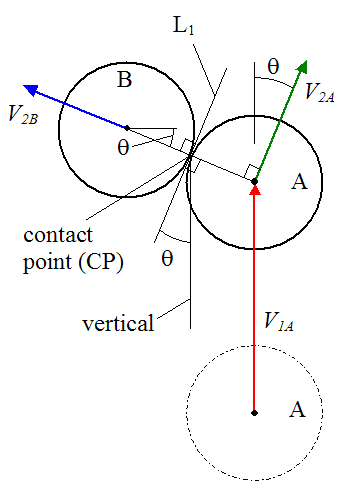
\includegraphics[scale = 0.5]{Images/ballToBallCollisions.png}
    \caption{The direction vectors associated with each ball when a ball in motion, \(A\), collides with a stationary ball, \(B\). \cite{PhysicsOfBilliards}}
    \label{fig:balltoballcoll}
\end{figure}

Figure \ref{fig:balltoballcoll} shows a ball in motion, \(A\), with initial velocity \(V\textsubscript{1A}\) colliding with a stationary ball, \(B\). After the collision, ball \(B\) has velocity \(V\textsubscript{2B}\), whilst ball \(A\) has velocity \(V\textsubscript{2A}\). We can see that vector \(V\textsubscript{2B}\) points in the same direction as a straight line drawn from the centre of ball \(A\) through to the centre of ball \(B\) at the exact time of collision. We can also see that vector \(V\textsubscript{2A}\) is perpendicular to vector \(V\textsubscript{2B}\) \cite{PhysicsOfBilliards}. Due to the nature of my application, we do not need to worry about the speed of either ball post collision, as we are only interested in approximating their direction, not how far they will travel. Therefore, assuming that the centre points of both balls are known at the time of collision we can calculate their post collision directions.\\

Despite the above being correct, this is only the case for what is known as a \textit{Stun Shot}; where the cue ball (ball \(A\) in Figure \ref{fig:balltoballcoll}) has no spin in any direction. In reality however, most non-technical shots will naturally apply top-spin onto the cue ball causing it not to travel in the direction of \(V\textsubscript{2A}\). Therefore, another way of estimating the angle for the cue ball post collision will be required. 

\subsection{Ball-To-Rail Collisions}
The other type of collision we must consider is between a ball and the rail (or cushion) of the table. Unlike ball-to-ball collisions, ball-to-rail collisions are not and cannot be considered as elastic, 


\begin{figure}[h!]
    \centering
    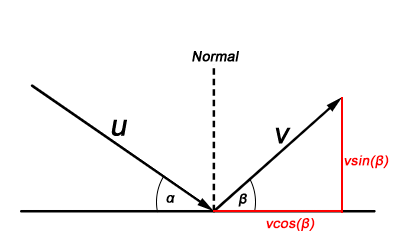
\includegraphics[scale = 0.5]{Images/Ball-Cushion-Collision.png}
    \caption{The direction vectors associated with a ball colliding with the rail of the table. The vector \(u\) depicts the ball's initial velocity, and vector \(v\) depicts the ball's velocity post collision.}
    \label{fig:ballToRailColl}
\end{figure}



% ~ 10 pages

% \noindent
% This chapter is intended to describe the technical basis on which execution
% of the project depends.  The goal is to provide a detailed explanation of
% the specific problem at hand, and existing work that is relevant (e.g., an
% existing algorithm that you use, alternative solutions proposed, supporting
% technologies).  

% Per the same advice in the handbook, note there is a subtly difference from
% this and a full-blown literature review (or survey).  The latter might try
% to capture and organise (e.g., categorise somehow) {\em all} related work,
% potentially offering meta-analysis, whereas here the goal is simple to
% ensure the dissertation is self-contained.  Put another way, after reading 
% this chapter a non-expert reader should have obtained enough background to 
% understand what {\em you} have done (by reading subsequent sections), then 
% accurately assess your work.  You might view an additional goal as giving 
% the reader confidence that you are able to absorb, understand and clearly 
% communicate highly technical material.

% -----------------------------------------------------------------------------

\chapter{Project Execution}
\label{chap:execution}

% {\bf A topic-specific chapter, of roughly $15$ pages} 
% \vspace{1cm} 

% \noindent
% This chapter is intended to describe what you did: the goal is to explain
% the main activity or activities, of any type, which constituted your work 
% during the project.  The content is highly topic-specific, but for many 
% projects it will make sense to split the chapter into two sections: one 
% will discuss the design of something (e.g., some hardware or software, or 
% an algorithm, or experiment), including any rationale or decisions made, 
% and the other will discuss how this design was realised via some form of 
% implementation.  

% This is, of course, far from ideal for {\em many} project topics.  Some
% situations which clearly require a different approach include:

% \begin{itemize}
% \item In a project where asymptotic analysis of some algorithm is the goal,
%       there is no real ``design and implementation'' in a traditional sense
%       even though the activity of analysis is clearly within the remit of
%       this chapter.
% \item In a project where analysis of some results is as major, or a more
%       major goal than the implementation that produced them, it might be
%       sensible to merge this chapter with the next one: the main activity 
%       is such that discussion of the results cannot be viewed separately.
% \end{itemize}

% \noindent
% Note that it is common to include evidence of ``best practice'' project 
% management (e.g., use of version control, choice of programming language 
% and so on).  Rather than simply a rote list, make sure any such content 
% is useful and/or informative in some way: for example, if there was a 
% decision to be made then explain the trade-offs and implications 
% involved.


% \begin{figure}[t]
% \centering
% foo
% \caption{This is an example figure.}
% \label{fig}
% \end{figure}

% \begin{table}[t]
% \centering
% \begin{tabular}{|cc|c|}
% \hline
% foo      & bar      & baz      \\
% \hline
% $0     $ & $0     $ & $0     $ \\
% $1     $ & $1     $ & $1     $ \\
% $\vdots$ & $\vdots$ & $\vdots$ \\
% $9     $ & $9     $ & $9     $ \\
% \hline
% \end{tabular}
% \caption{This is an example table.}
% \label{tab}
% \end{table}

% \begin{algorithm}[t]
% \For{$i=0$ {\bf upto} $n$}{
%   $t_i \leftarrow 0$\;
% }
% \caption{This is an example algorithm.}
% \label{alg}
% \end{algorithm}

% \begin{lstlisting}[float={t},caption={This is an example listing.},label={lst},language=C]
% for( i = 0; i < n; i++ ) {
%   t[ i ] = 0;
% }
% \end{lstlisting}
\section{Deployment Requirements and Set-Up}
\label{exec:deployment}

\section{Application Models}
\label{exec:modelling}

\section{User Interface and Interaction}
\label{exec:UI}

\section{Object Placement}
\label{exec:objectPlacement}

\section{Post Collision Direction Estimation and Path Drawing}
\label{exec:collisionPath}
\subsubsection{Finding The Coefficient of Restitution of The Pool Table}

\section{Hologram Stabilisation}
\label{exec:holoStabilisation}


% -----------------------------------------------------------------------------

\chapter{Critical Evaluation}
\label{chap:evaluation}

Throughout this chapter, each major part of the aim assistant application were tested and evaluated in order to gauge the success of the project, as well as its usefulness and usability. Within each section, details of the experiments performed and discussion of the subsequent results are present in order to give a contextual, in-depth overview of the findings.

\section{Hologram Stability}
\label{eval:stability}

A major part of the application working well, and being effective in improving the user's potting accuracy, is for the holographic content to stay in place whilst the user moves around the room. As most of the holographic content is placed over the top of real life objects, i.e. the balls and table, if they were to move out of alignment then the user would not be able to line up a shot accurately, making the application less effective.
Some mitigations were taken in order to try and reduce the amount holograms move about as the user moves, as detailed in Section \ref{exec:holoStabilisation}, and it is important to see how effective these were in stabilising the holograms the application displays. In order to determine how drastic this movement (or \textit{drift}) is, and to what extent it interferes with someone using the system, the following experiments detailed in the sub-sections below were performed. Their main goal was to try and imitate what a user would typically do whilst planning and taking a shot, as well as some other common movements or environment changes that any HoloLens wearer could experience regardless of the application that they were using. \\

Whilst the HoloLens is capable of taking photos and videos capturing what the user sees, there is an apparent offset whilst doing so \cite{holographicDrift}. Although the user will see that the content is aligned, in said MR photo/video content this is often not the case, with the holograms appearing positioned up and to the left of where they actually are at distances of greater than approximately one meter. As such, most captured content cannot be used to accurately evaluate any holographic drifting that may occur. An effort was made to try and reduce or eliminate this offset effect using the techniques advised by Microsoft \cite{hololensFocusPoint}\cite{mixedRealityCapture}, however the issue still persisted after the fact. It is apparent that for Microsoft's newest HoloLens device, the HoloLens 2, there is a way for developers to enable rendering of the holographic material from the point of view of the photo-video camera, which ensures MR captured content is aligned at any distance\cite{hololensPVrender}. However, I did not have a HoloLens 2 available to me and so this could not be tested nor verified.\\

To get around not being able to capture content from the user's perspective, an alternative evaluation method has been devised which was used for all experiments detailed in the sub-sections below. This method is as follows:
\begin{enumerate}
    \item A camera was placed in a single position throughout testing such that it had a clear view of the entire table.
    \item After starting my application and placing the table model into place, I place a holographic ball onto the table in any location.
    \item I then place a real life ball in the exact position of the holographic ball, leave it for a few seconds so that the camera can record it in position, then remove it.
    \item From here I perform the necessary actions that I am evaluating before returning to the table.
    \item Then I again place the real ball in the exact position that I see the holographic ball and leave it for a few seconds so that the camera can record it in position.
    \item With these recorded positions, I can extract single frames from the video of each time I placed the real ball and compare its position between frames.
\end{enumerate}

Using this method, we can compare the ball positions between the frames either visually, or by aligning and superimposing them onto each other. If there is little to no movement of the ball between the aligned frames then the holograms are stable. However, if there is drastic differences between the ball's position in the frames then we will know that the holograms are not stable under the tested conditions. To maintain accuracy, the camera position was fixed throughout each test and I carried out each test to not introduce any variation between ball placement or judgement of where the ball is.

\subsection{Movement Around the Table}
In order to test how stable the holograms would be whilst a user was walking around the table, like they would do in a game or when practicing, I lined up the real ball with where I saw the holographic one from each side of the table. Figure \ref{fig:evalTableMovement} shows the ball's apparent position from the left, top, right, and bottom edges of the table from one of the five test repetitions, each of which yielded consistent results.

\begin{figure}[h!]
    \centering
    \begin{tabular}{cc}
         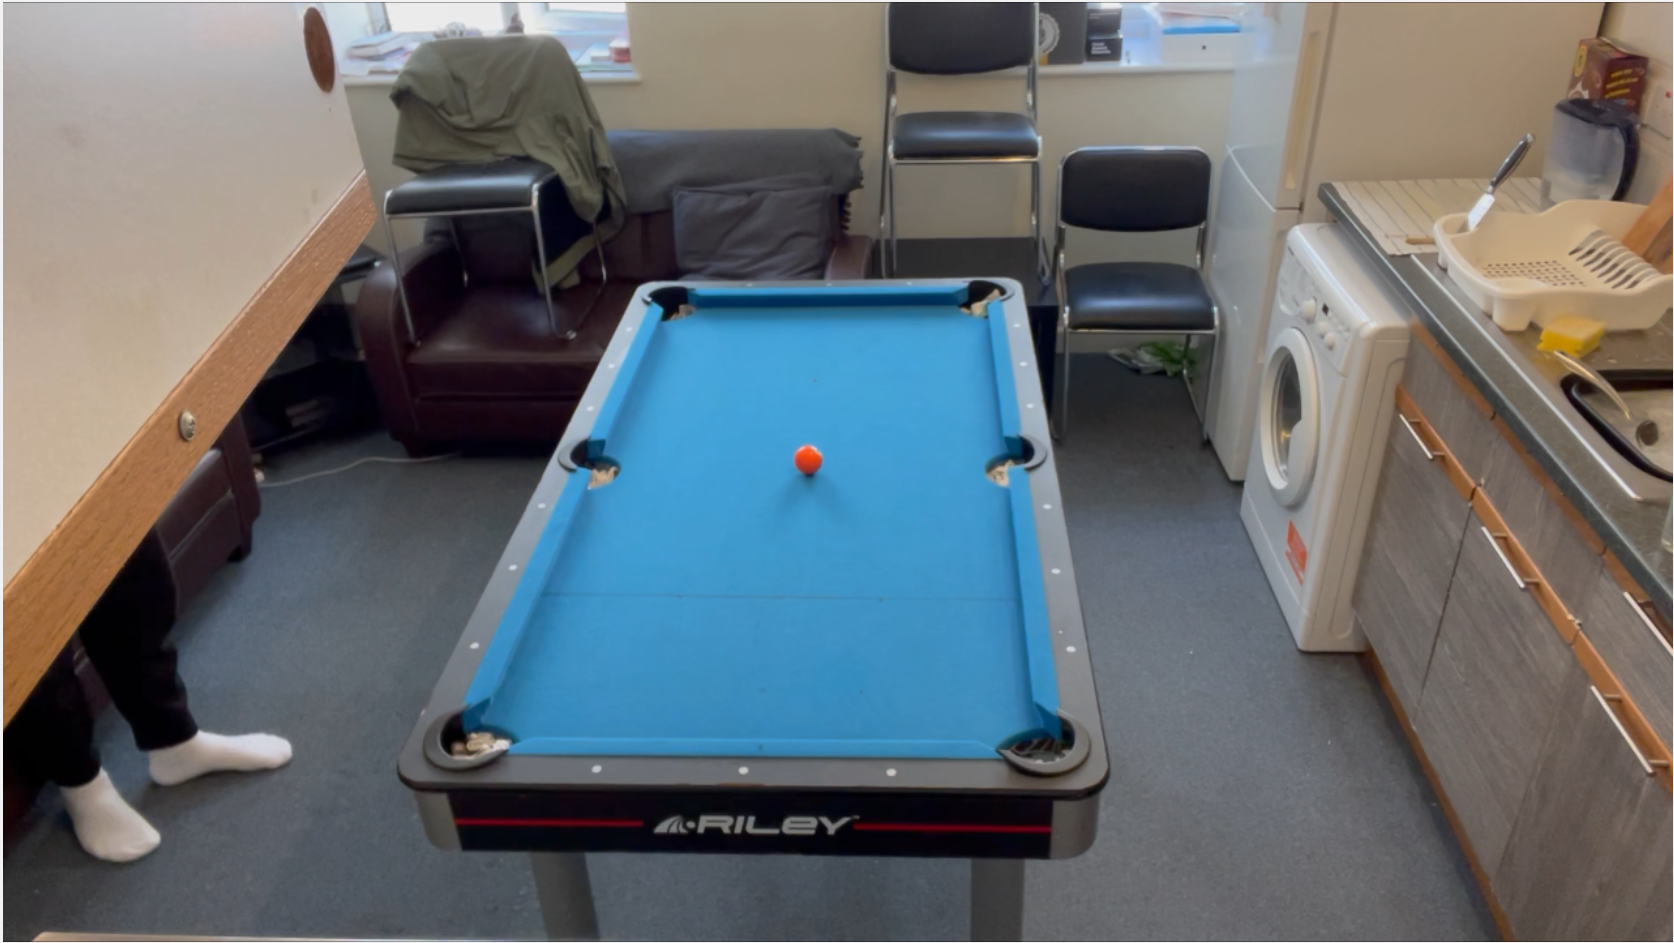
\includegraphics[scale = 0.15]{Images/Eval/Walk around/Frame 5 - LHS 2.PNG} & 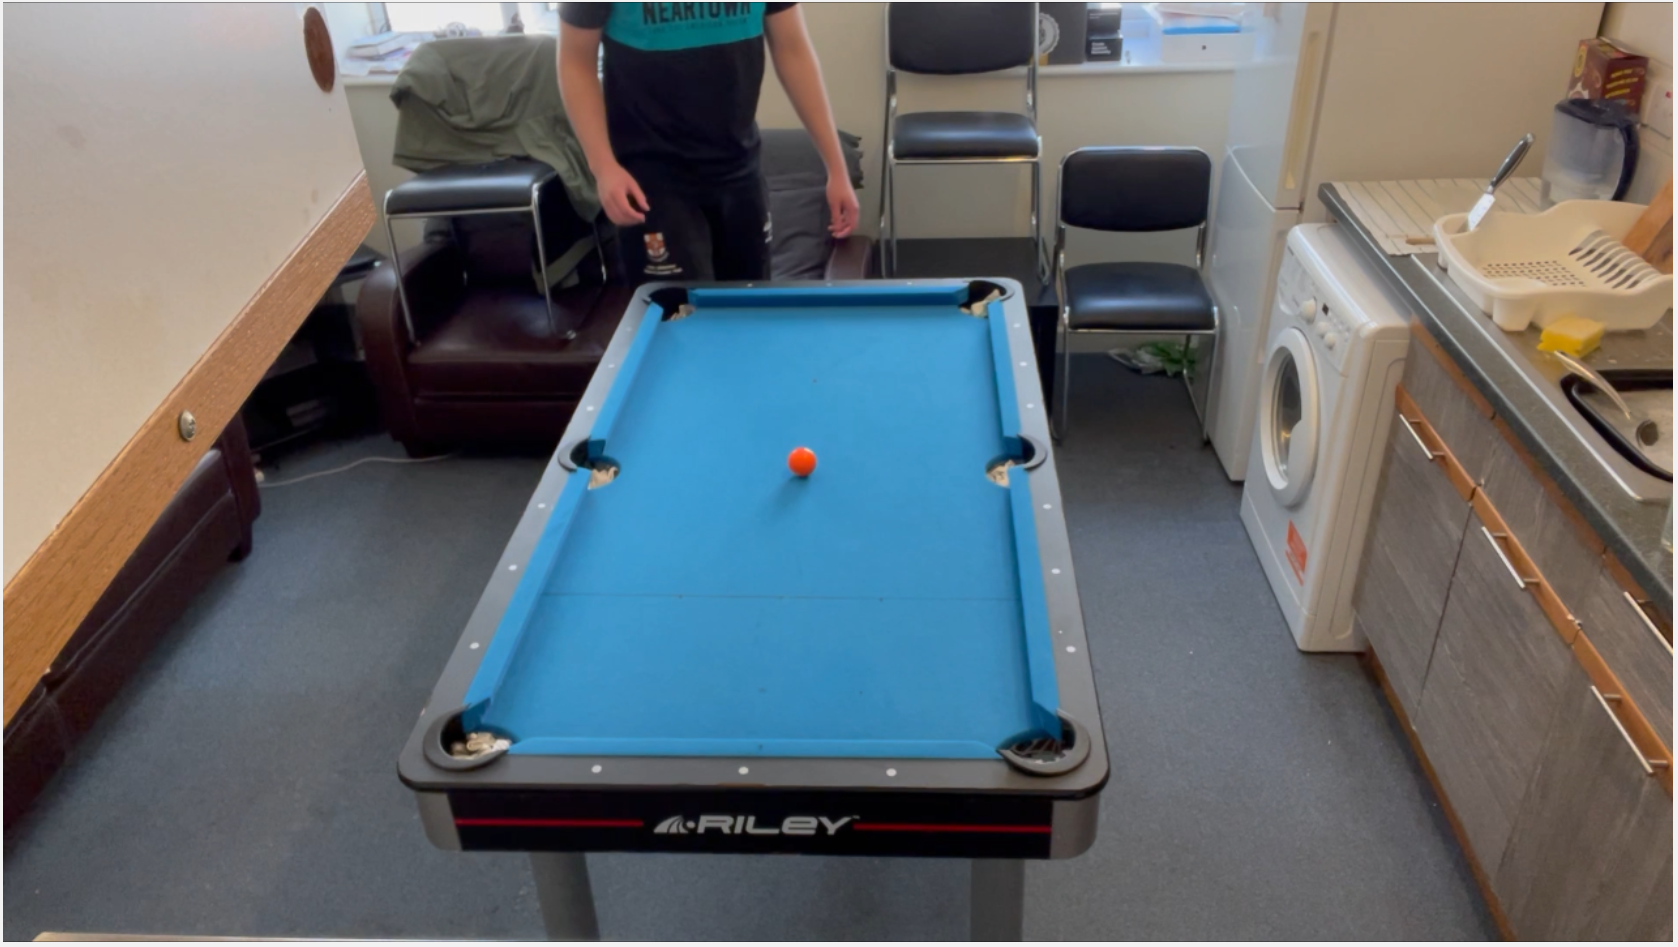
\includegraphics[scale = 0.15]{Images/Eval/Walk around/Frame 6 - Back 2.PNG} \\
         (a) Position 1 (LHS). & (b) Position 2 (TOP). \\[6pt]
         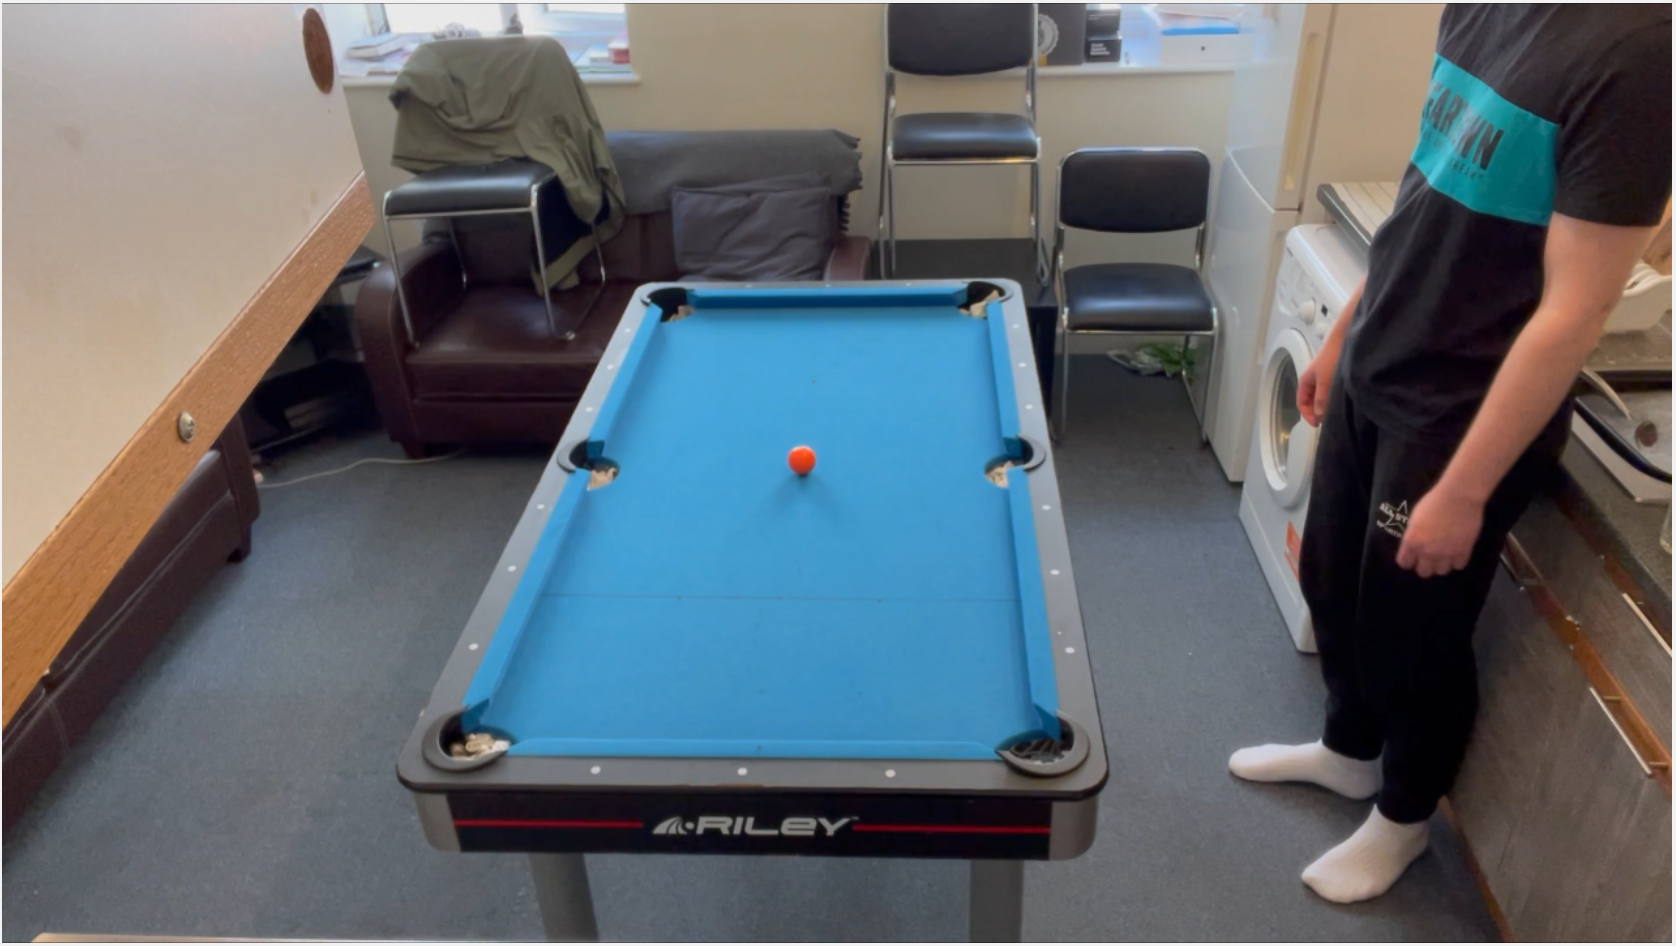
\includegraphics[scale = 0.15]{Images/Eval/Walk around/Frame 7 - RHS 2.PNG} & 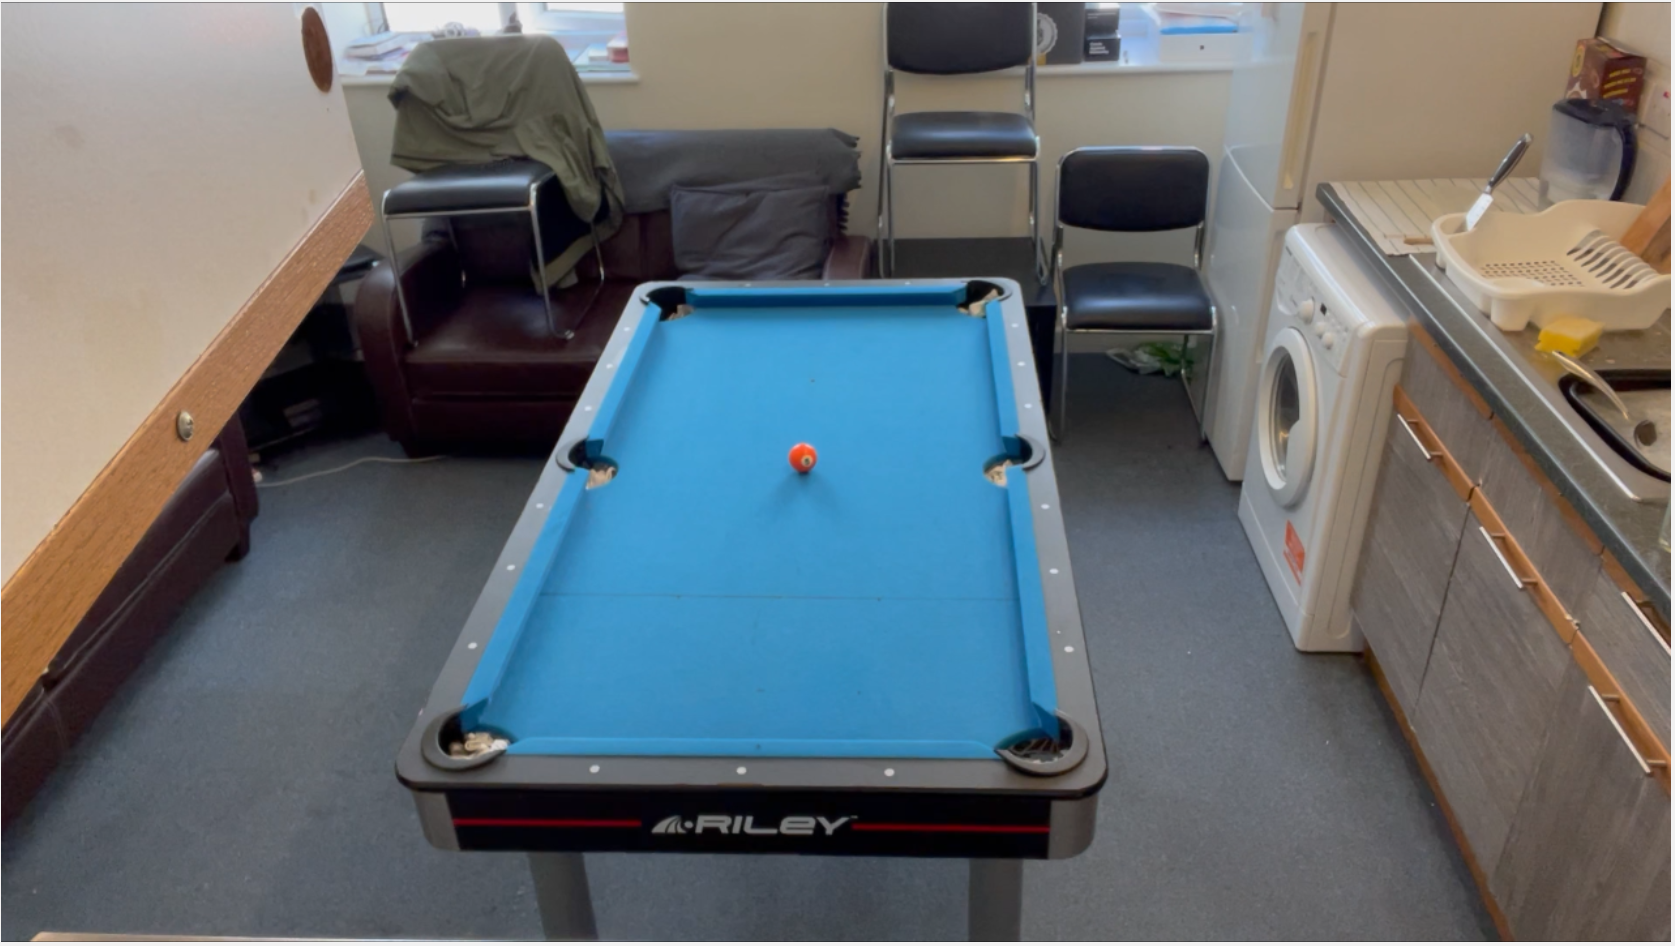
\includegraphics[scale = 0.15]{Images/Eval/Walk around/Frame 8 - Front 2.PNG} \\ 
         (c) Position 3 (RHS). & (d) Position 4 (BOT). \\[6pt]
         \multicolumn{2}{c}{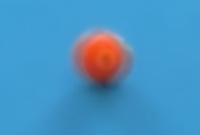
\includegraphics[scale = 0.7]{Images/Eval/Walk around/Walk about overlay 2.png}} \\
         \multicolumn{2}{c}{(e) All balls from frames superimposed. }
    \end{tabular}
    \caption{The above images show where the holographic ball was seen in each position. These have been superimposed in image (e) to allow for easier recognition of any drift that has occurred.}
    \label{fig:evalTableMovement}
\end{figure}

From panel (e) in Figure \ref{fig:evalTableMovement}, we can see that there was some minor movement between each of the four positions of up to approximately a quarter of the ball's diameter, or 12.5mm. This is clearly not ideal, especially for thin cut shots, as the user's shot that they have lined up will not be accurate due to the drift that has occurred. The user can correct this by moving the ball's back into place before they take their shot, but this is not ideal and is likely to frustrate them over time. Although we are unable to test or evaluate if the table hologram has also drifted, we can assume that if the balls have experienced drift then so has the table. This is because all ball objects are children of the table object, meaning that they are subject to the \textit{spacial anchor} attached to the table \cite{WMRinputAnchors}. Whilst in theory the \textit{spacial anchor} should keep the holograms in the exact place they were left, it is clear that this has not happened exactly from the drift apparent in panel (e). It will become clear in Section \ref{eval:pathAccuracy} whether or not this minor drift caused by moving around the table has any effect on the accuracy of the path prediction system.


\subsection{Major Environmental Changes}
For this test, I wanted to see how the HoloLens and the holograms it displays reacted to environmental changes, such as leaving the room briefly and returning. Microsoft states that tracking can be effected due to dynamic changes in the environment, such as people walking around the room\cite{environmentChangesPeople} or significant movement of known objects such as furniture\cite{environmentChangesfurniture}. What isn't clear is how an addition to the known environment, like walking into another room, will effect the HoloLens' tracking and subsequently the position of any holograms. In order to give the best chances if success, an ideal testing condition environment was used as detailed by Microsoft\cite{hololensEnvironmentConsiderations}. Therefore, adequate lighting was used, no objects within either room were moved, no other people were moving around the rooms, and both rooms had a large number of objects to help improve tracking. 

\begin{figure}[h!]
    \centering
    \begin{tabular}{cc}
         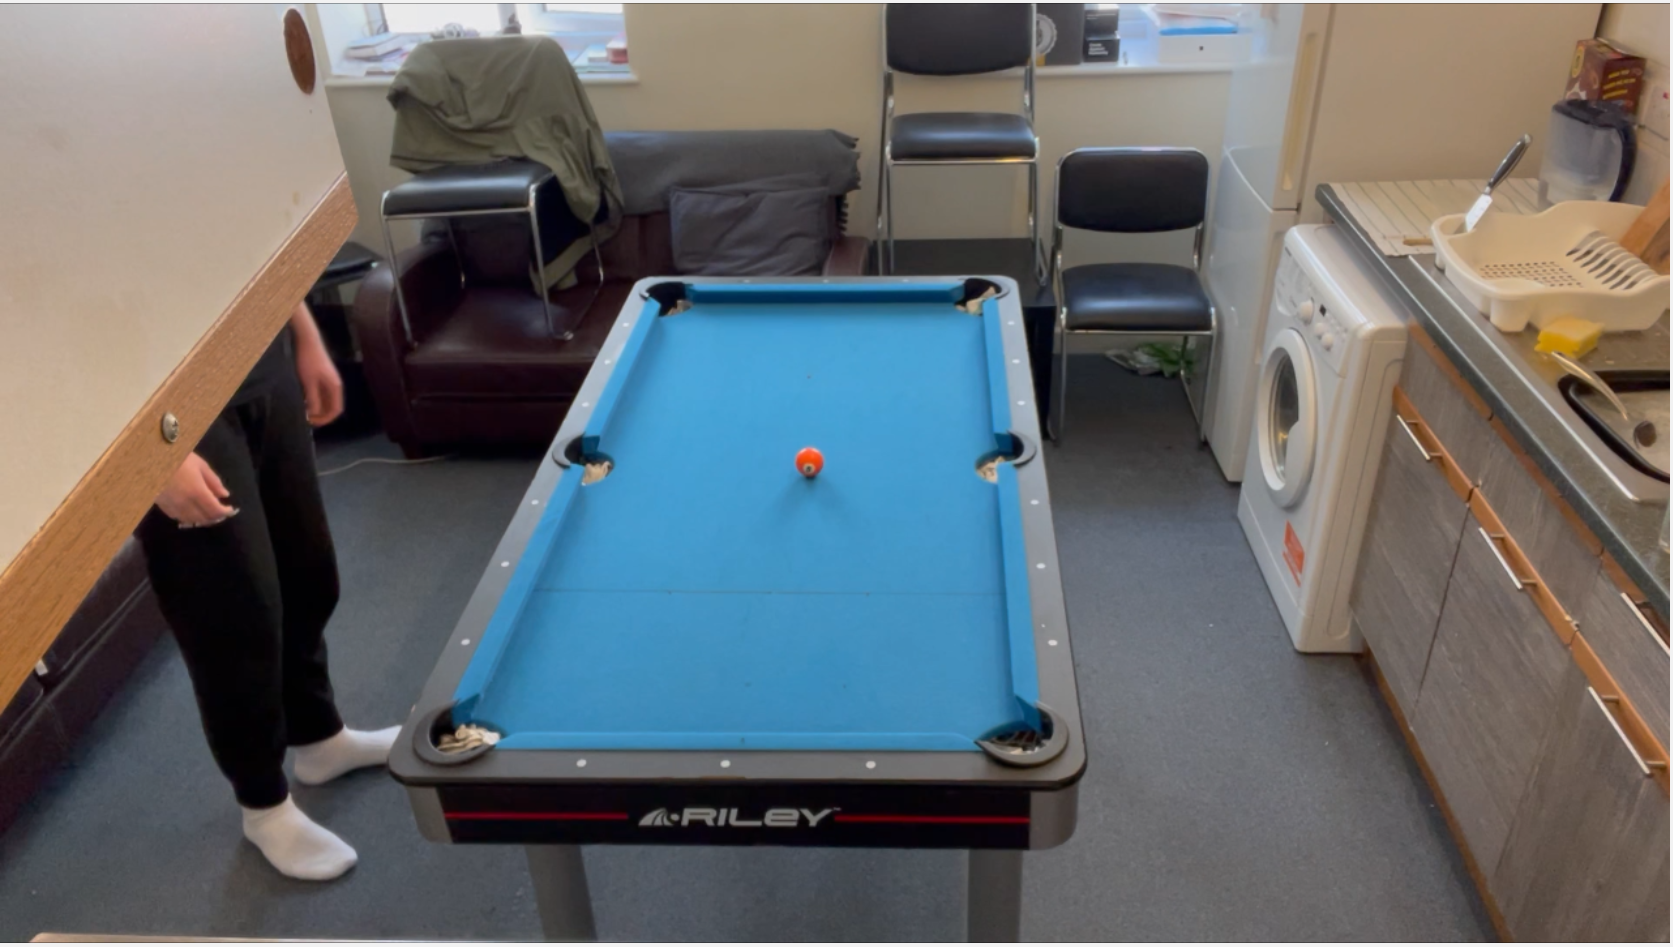
\includegraphics[scale = 0.15]{Images/Eval/Leave Room/Frame 1 - 0 leaves.PNG} & 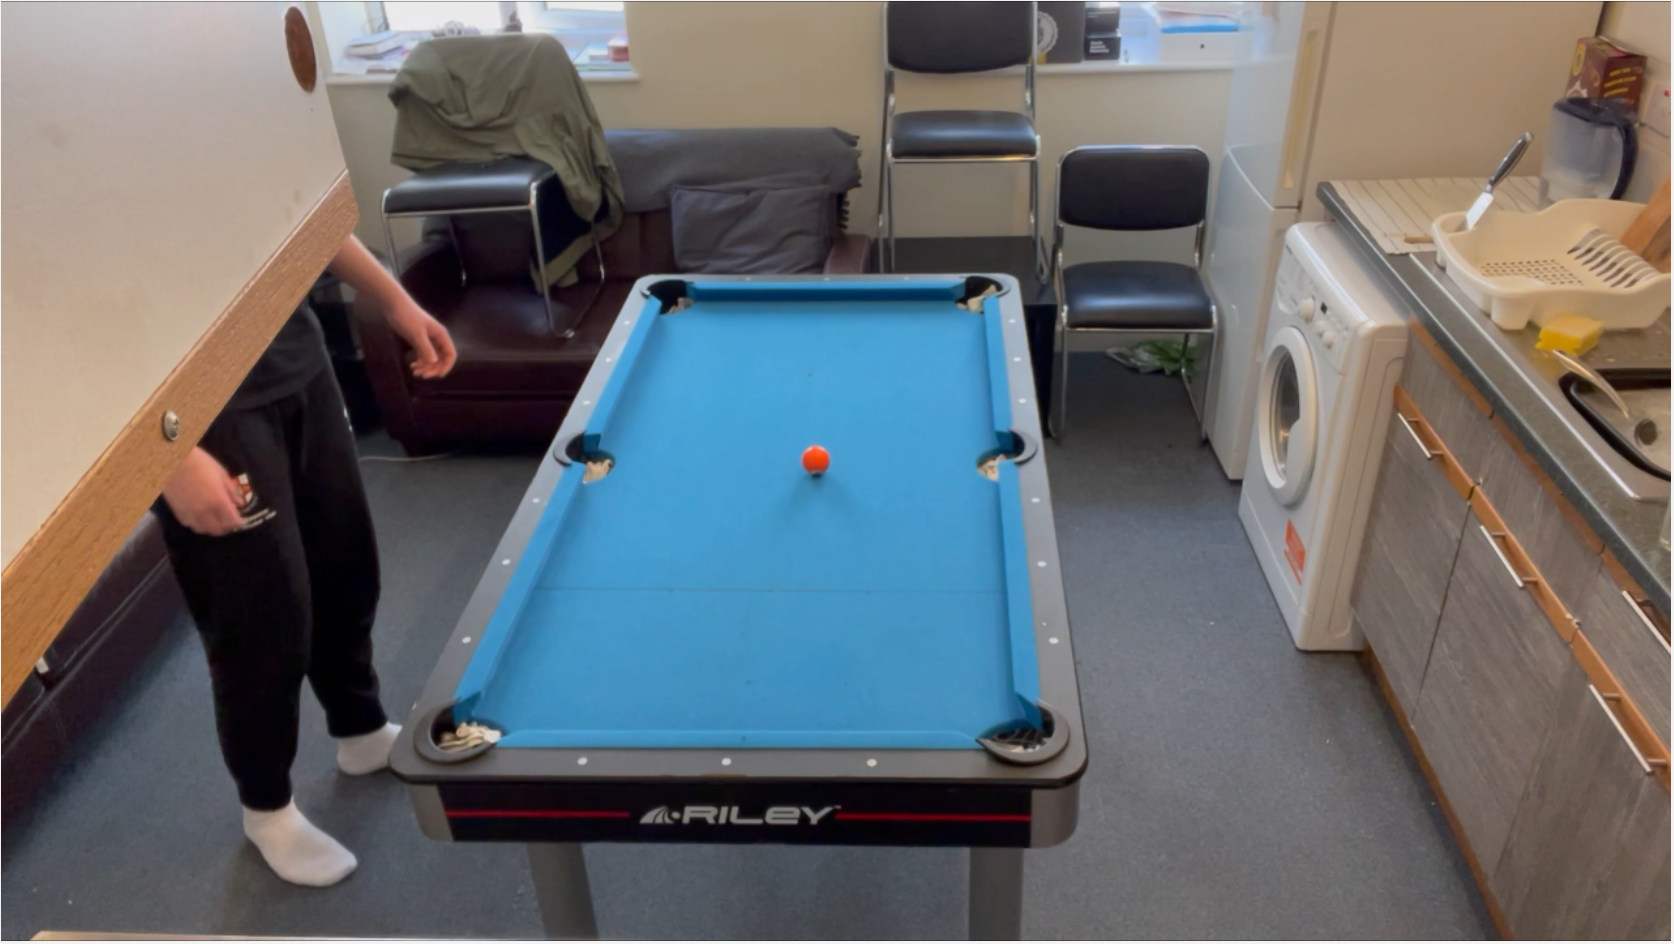
\includegraphics[scale = 0.15]{Images/Eval/Leave Room/Frame 2 - 1 leaves.PNG} \\
         (a) Initial position. & (b) Position after leaving the room once. \\[6pt]
         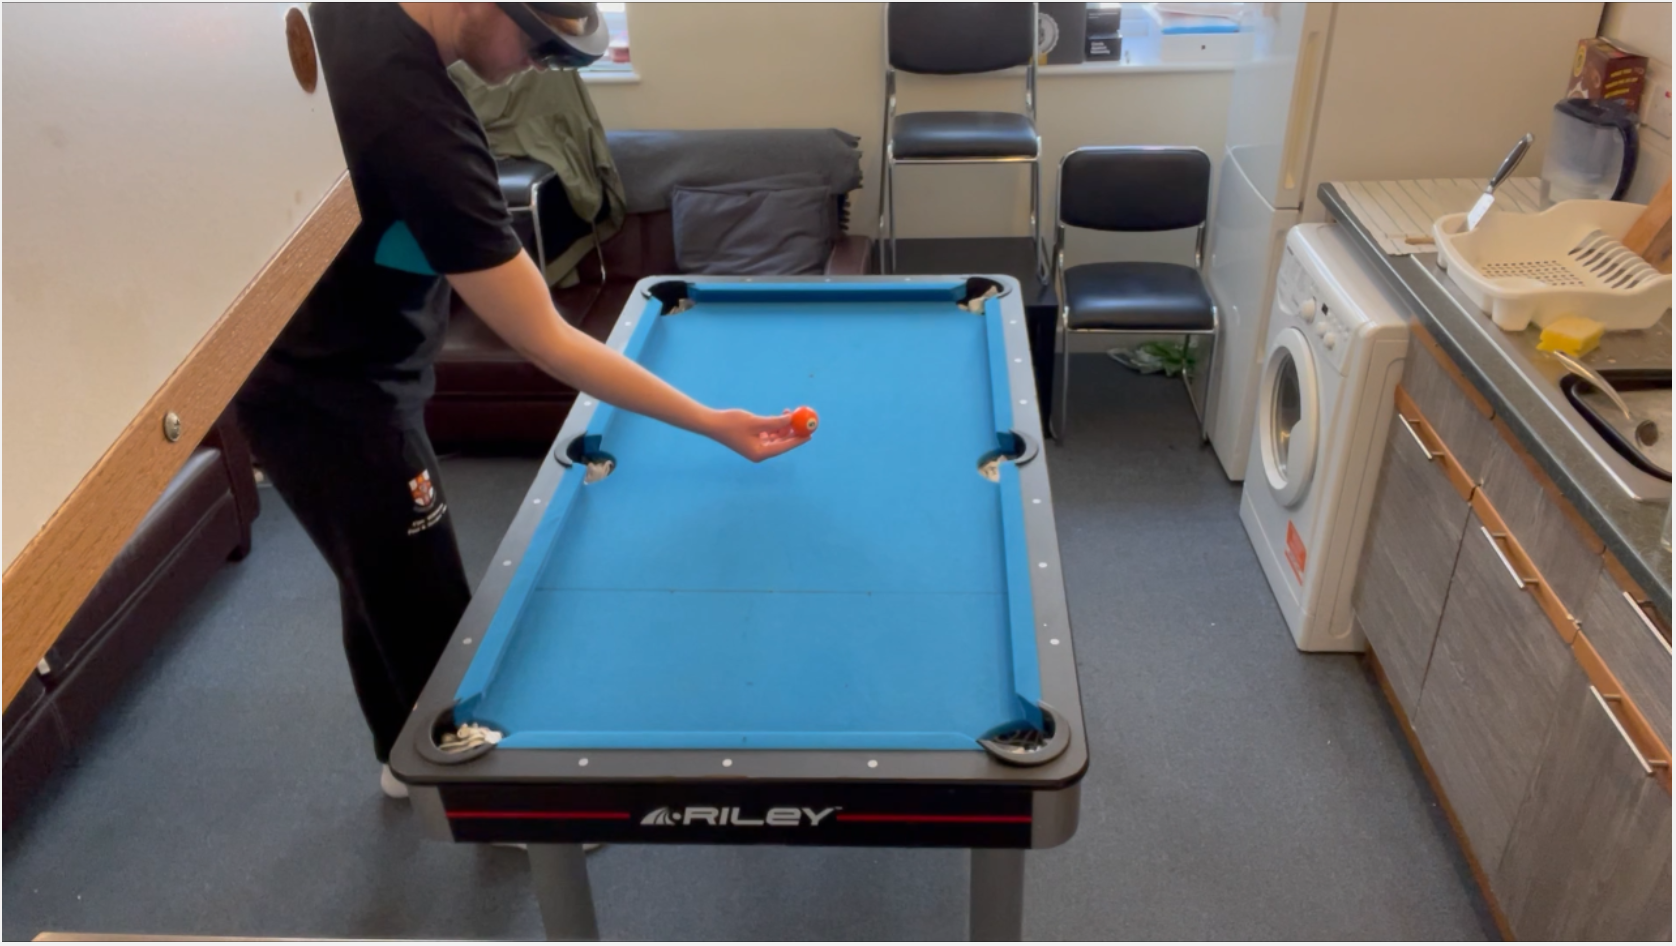
\includegraphics[scale = 0.15]{Images/Eval/Leave Room/Frame 3 - 2 leaves.PNG} & 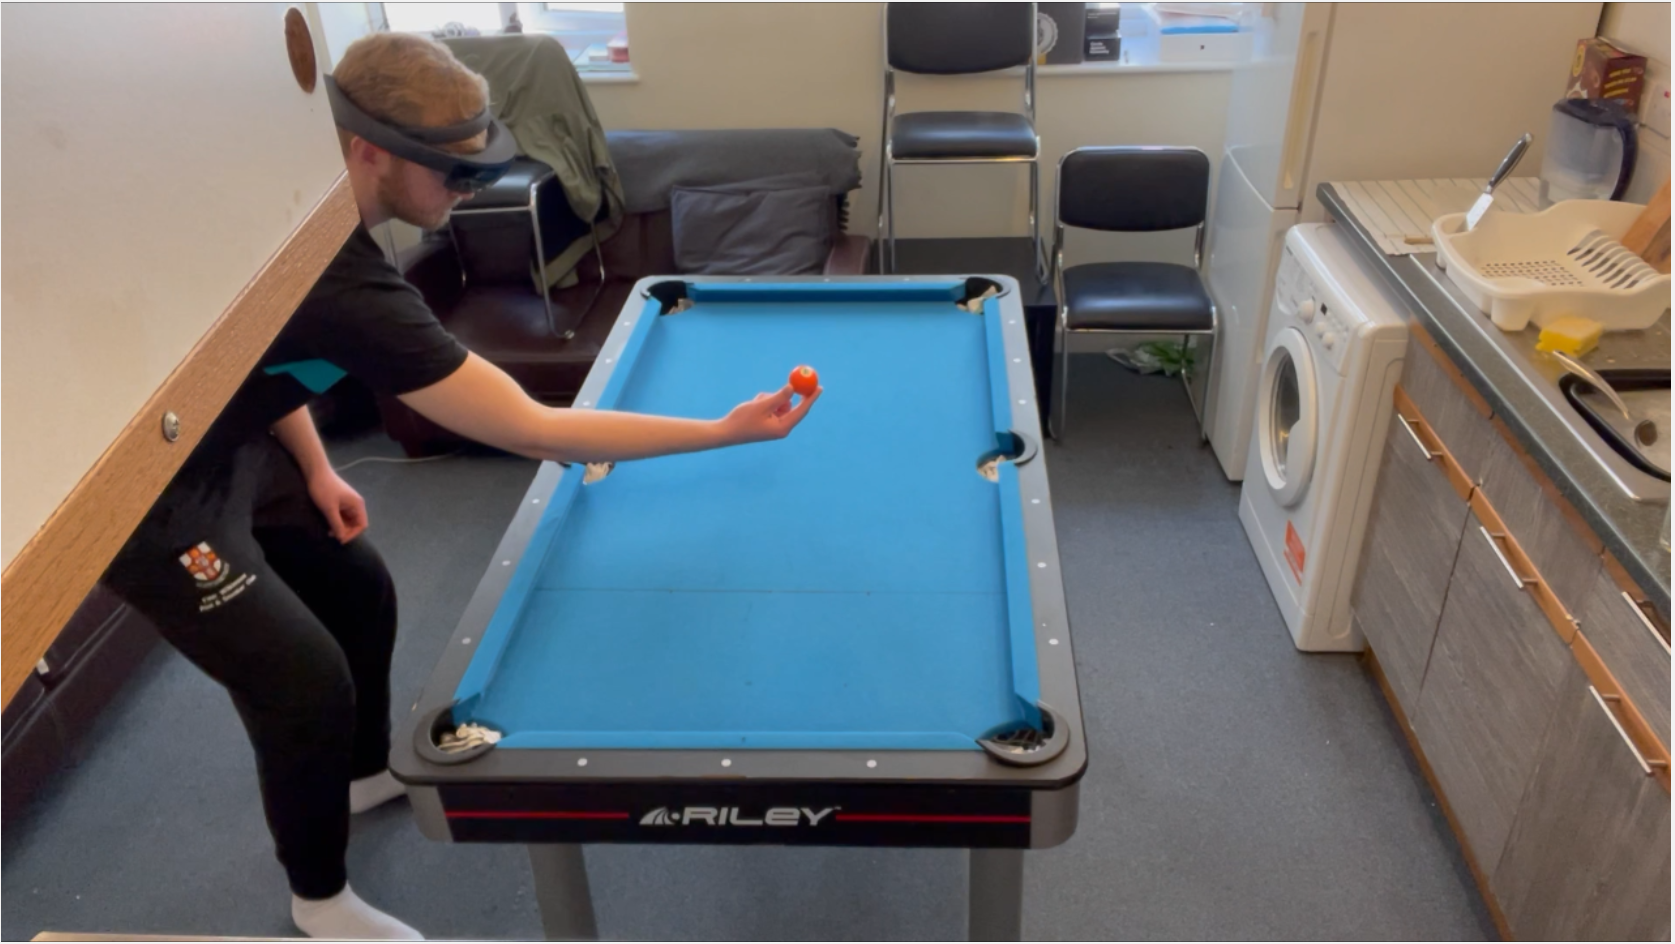
\includegraphics[scale = 0.15]{Images/Eval/Leave Room/Frame 5 - 3 leaves.PNG} \\ 
         (c) Position after leaving the room twice. & (d) Position after leaving the room thrice. \\[6pt]
         \multicolumn{2}{c}{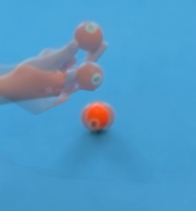
\includegraphics[scale = 0.5]{Images/Eval/Leave Room/All frames overlay.png}} \\
         \multicolumn{2}{c}{(e) All balls from the above images superimposed.}
    \end{tabular}
    \caption{The images above show the position of the holographic ball after leaving and re-entering the room a number of times. These have been superimposed in image (e) to allow for easier recognition of any drift that has occurred.}
    \label{fig:evalLeaveRoom}
\end{figure}

Figure \ref{fig:evalLeaveRoom} shows the position of the holographic ball, represented to the camera by placing the real ball in the same location, after leaving the room and returning three times. Just from comparing panels (a) through (d), it is evident that this had a major effect to the tracking of the HoloLens causing substantial holographic drift. This is visualised more clearly in panel (e), where it can be seen that vertical drift is most apparent and lateral drift is kept fairly minimal. Interestingly, it seems that only leaving the room once had a similar impact to the hologram positions as moving around the table did, but on repeated exit and entry to the room there was more of an effect. Despite this, it becomes clear that once a user begins to use the aiming assistant that they should not leave the room whilst wearing the headset, else the application becomes unusable without a restart. 

\subsection{Removal of the Headset}
As with many head mounted displays, there are a proportion of users who experience discomfort, eye strain, and neck fatigue from extended use. This has been reported in previous studies where a HoloLens was used\cite{holoLesnComfortPaperExample}, and was also mentioned in the feedback from user testing that I carried out by at least one of the participants. As such, it may be common for a user to take breaks and remove the headset whilst they are using it. I wish to see what effect removing the HoloLens would have on the hologram stability and tracking if it were removed and placed down onto a surface upside-down whilst my aim assistant application was running. 

\begin{figure}[h!]
    \centering
    \begin{tabular}{cc}
         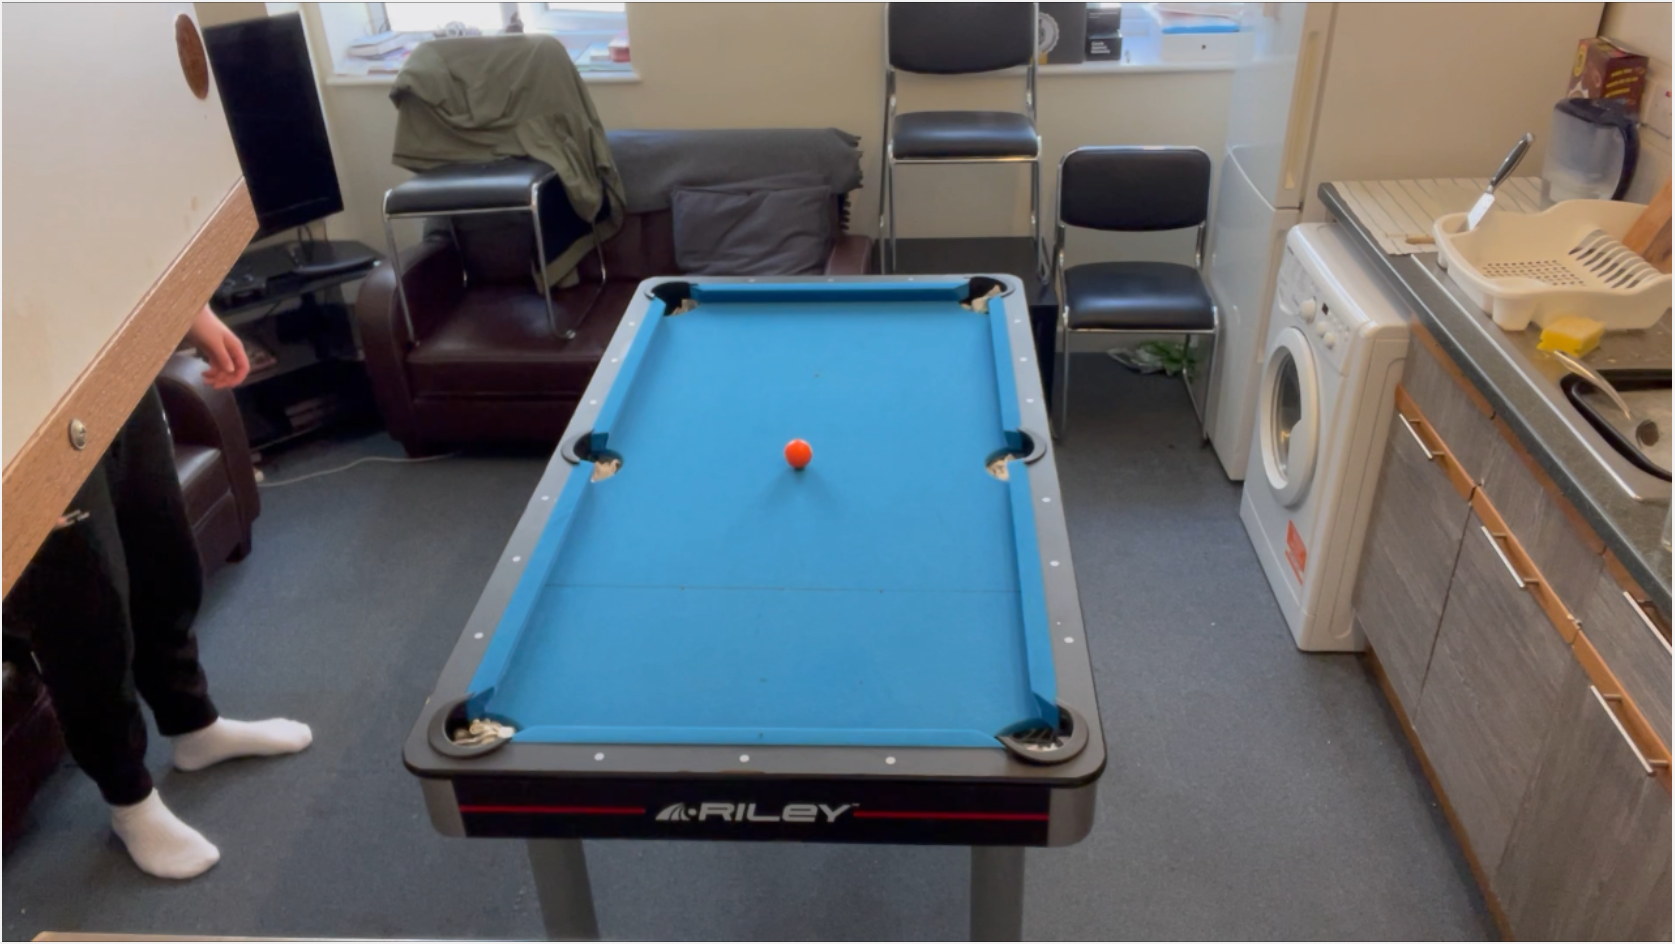
\includegraphics[scale = 0.15]{Images/Eval/Remove Headset/Frame 1 - 0 removes.PNG} & 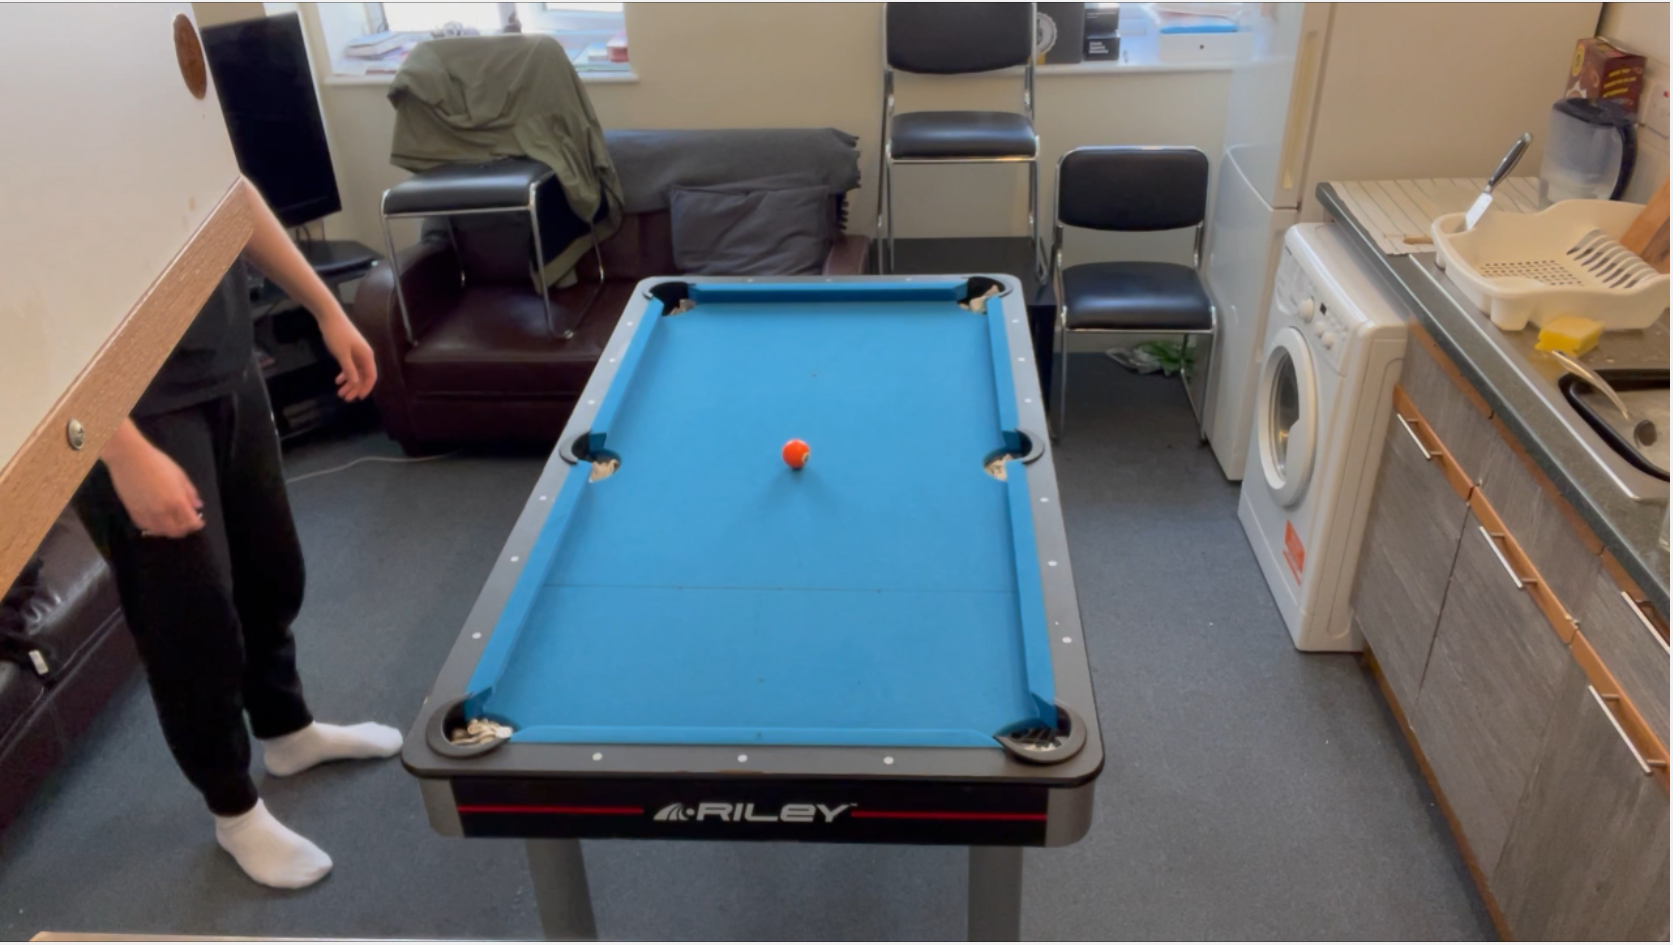
\includegraphics[scale = 0.15]{Images/Eval/Remove Headset/Frame 2 - 1 removes.PNG} \\
         (a) Initial position. & (b) Position after removing HoloLens once. \\[6pt]
         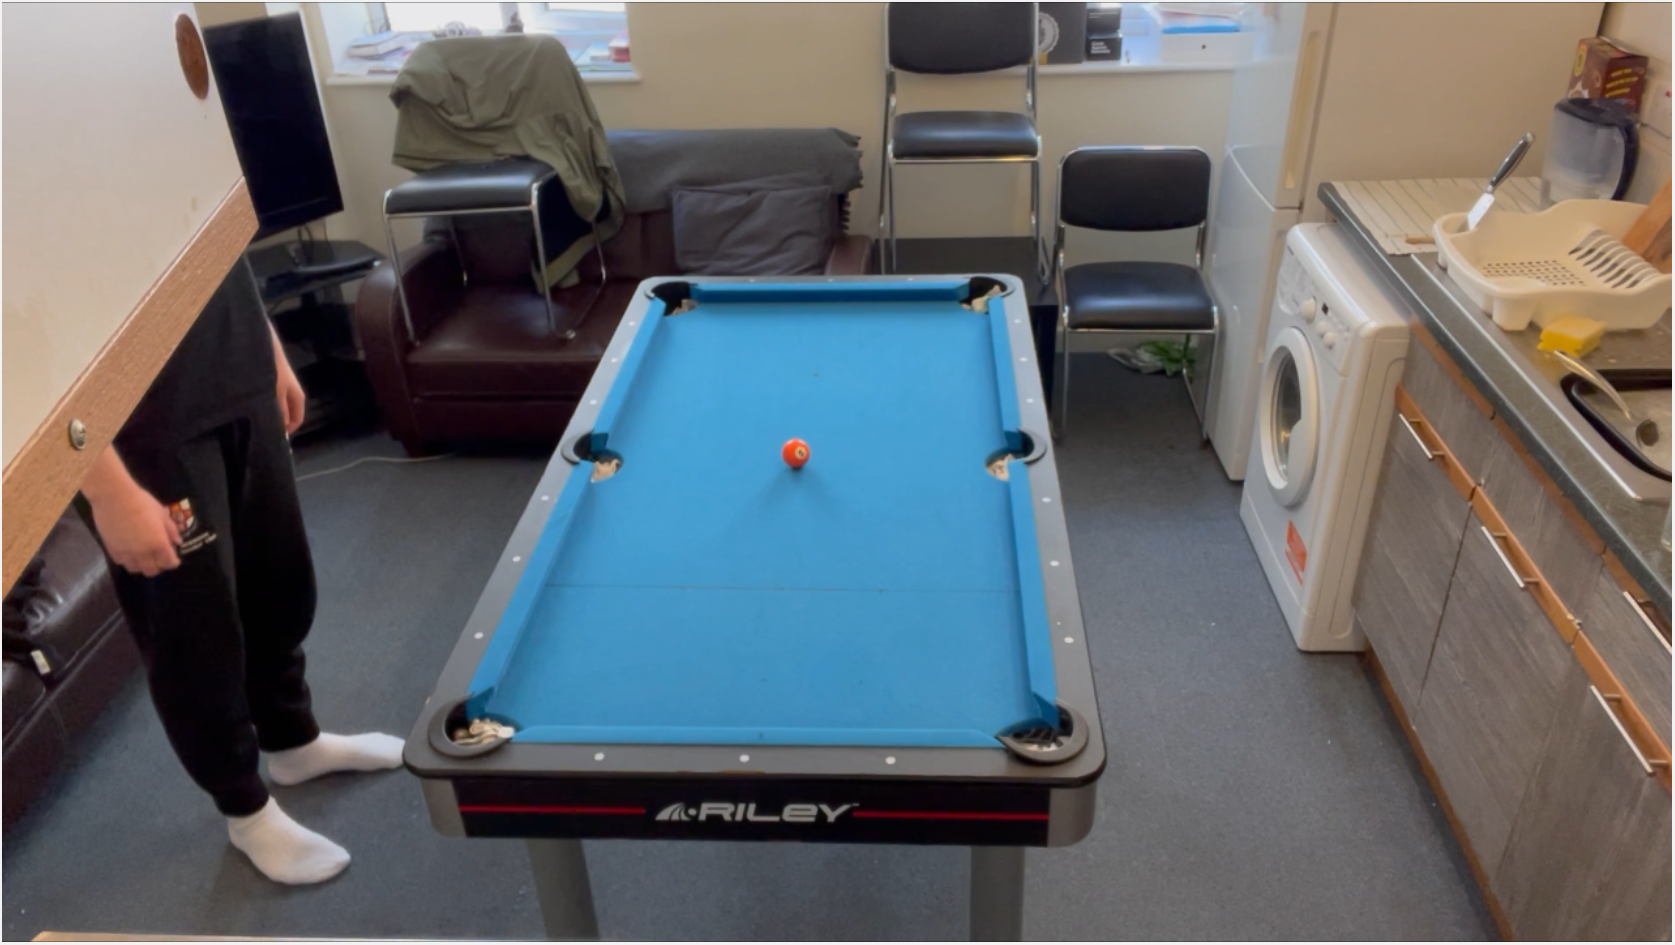
\includegraphics[scale = 0.15]{Images/Eval/Remove Headset/Frame 3 - 2 removes.PNG} & 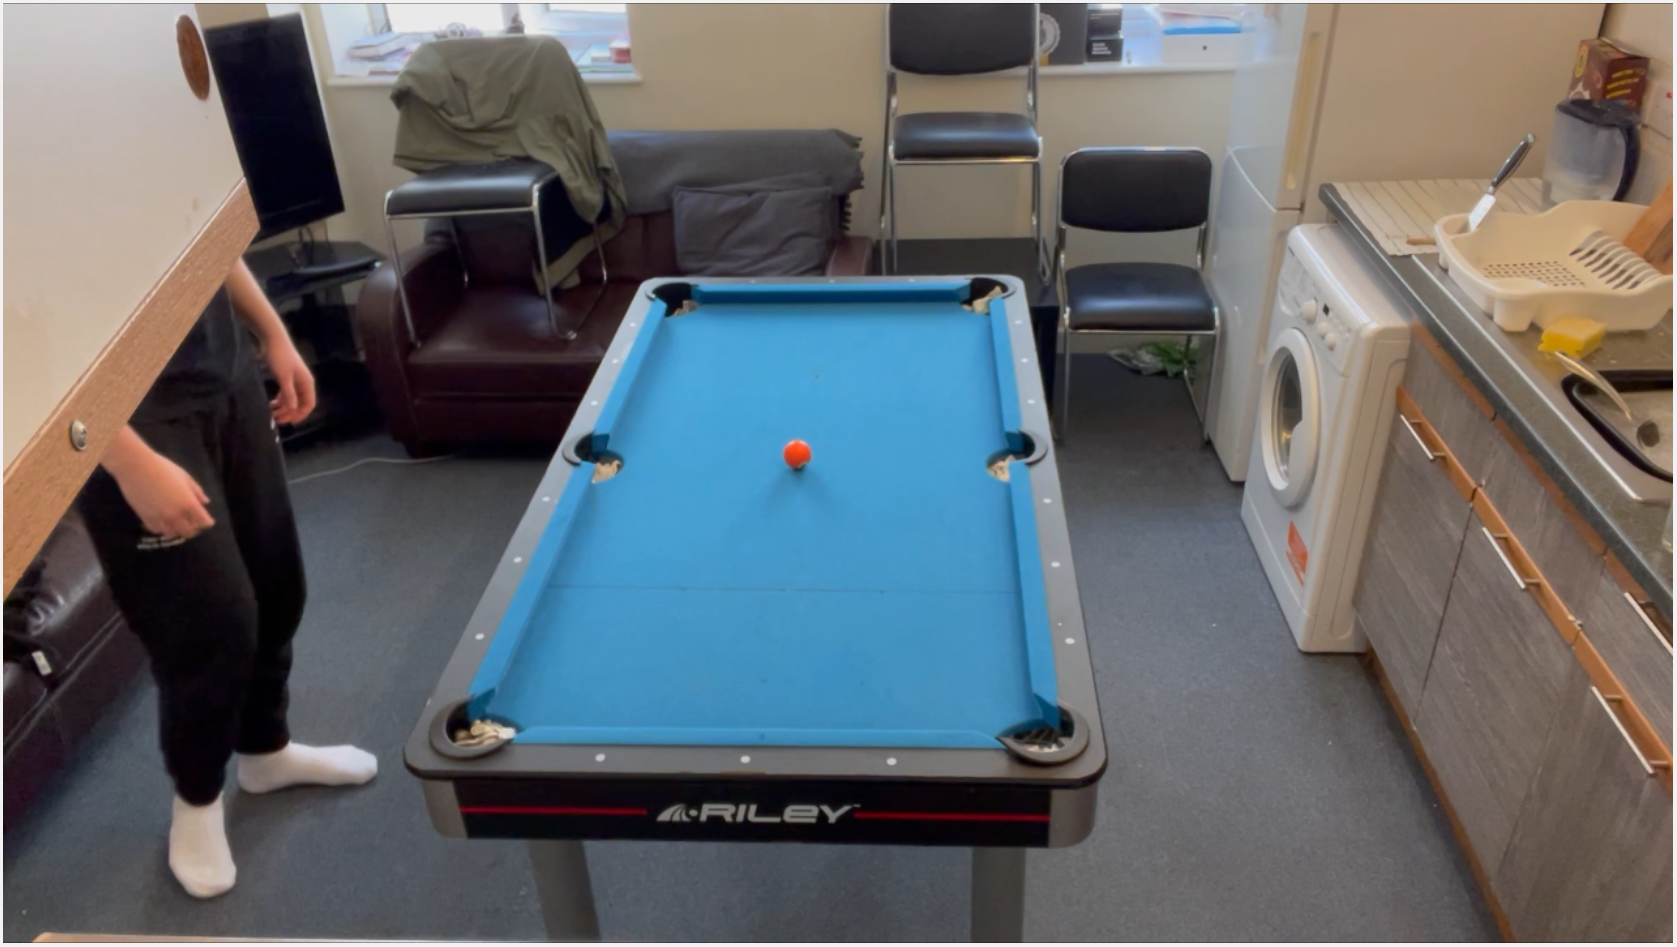
\includegraphics[scale = 0.15]{Images/Eval/Remove Headset/Frame 4 - 3 removes.PNG} \\ 
         (c) Position after removing HoloLens twice. & (d) Position after removing HoloLens thrice. \\[6pt]
         \multicolumn{2}{c}{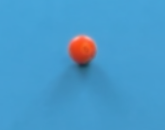
\includegraphics[scale = 0.7]{Images/Eval/Remove Headset/Remove headset overlay.png}} \\
         \multicolumn{2}{c}{(e) All balls from the above images superimposed.}
    \end{tabular}
    \caption{Shown above are the positions of the holographic ball after removing the HoloLens multiple times. These positions have been superimposed in image (e) to allow for easier recognition of any drift that has occurred.}
    \label{fig:evalRemoveHoloLens}
\end{figure}

Figure \ref{fig:evalRemoveHoloLens} shows the perceived position of the holographic ball from the left hand side of the table after removal of the HoloLens up to three times, each time placing the headset down in a different location in the room. Panel (e) depicts these positions superimposed on top of one another and as we can clearly see, removing and replacing the HoloLens causes no holographic drift. The only assumption made with this is that the user removed and replaced the HoloLens from approximately the same place. Whether moving about the room and replacing the headset in a different location would effect drift is unknown. However, as the room itself has not changed, and the headset is moving whilst being placed down, it is unlikely that replacing the headset in a different location would cause any additional holographic drift than perceived when simply moving around the table.


\subsection{Change in Headset Height}
The final stability test focuses on another common movement a player has when playing pool or snooker - leaning over to take the shot. When doing this, the user's head height changes and as such, so will the height of the HoloLens whilst the user is using my application. Any holographic drift that occurs under this action could have a large effect on the user's shot accuracy, as a change in the cue ball's position will also change the position of the hit marker causing the user to strike the cue ball in the wrong place. 

\begin{figure}[h!]
    \centering
    \begin{tabular}{c}
         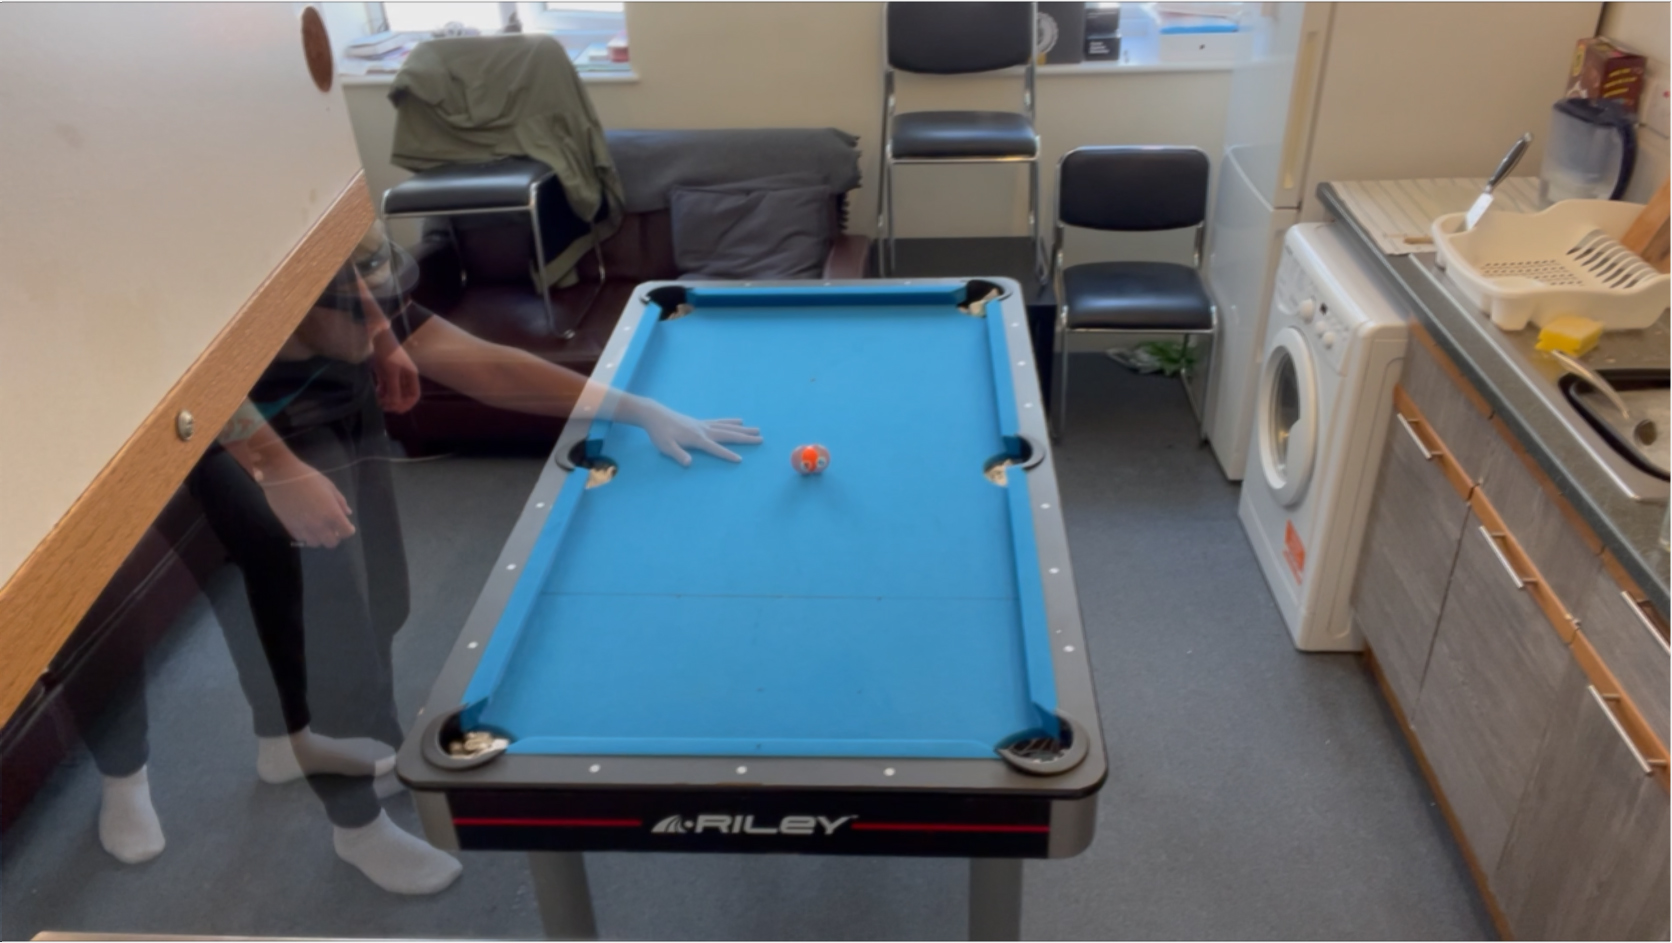
\includegraphics[scale = 0.17]{Images/Eval/Height Change/Pos1 overlay.png}\\
         (a) Superimposition of ball positions when standing and crouched - Position 1. \\[6pt]
         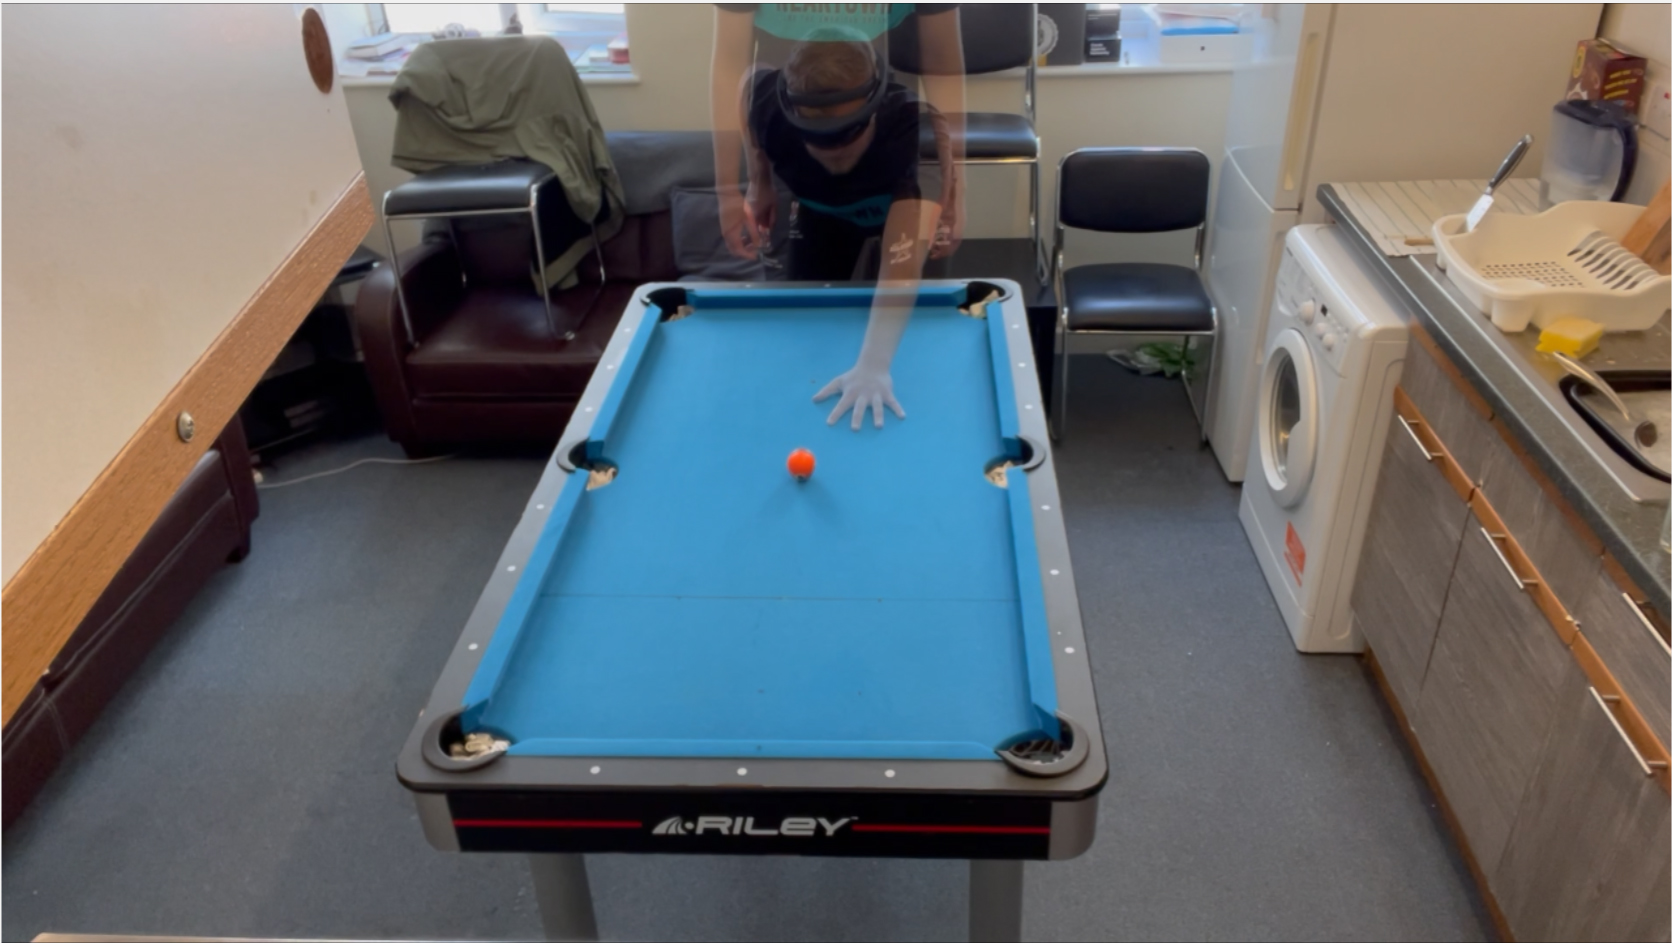
\includegraphics[scale = 0.17]{Images/Eval/Height Change/Pos2 overlay.png} \\
         (b) Superimposition of ball positions when standing and crouched - Position 4. \\[6pt]
    \end{tabular}
    \caption{Shown above are two repetitions of marking the holographic ball when standing and when crouched over (replicating the user taking a shot). The two stances have been superimposed in for each repetition to allow for easier recognition of any drift that has occurred.}
    \label{fig:evalHeadsetHeight}
\end{figure}

To evaluate this drift, I stood in 6 locations around the table and marked with a real ball where I perceived the holographic ball to be on the table. I then bent over into the shot-taking position and placed the ball again to mark the holograms position. Results from two of these tests can be seen in Figure \ref{fig:evalHeadsetHeight}, with each panel showing the standing and crouched ball positions superimposed on top of one another. Interestingly, when performing the task in position 1, shown by panel (a), there is some visible drift occurring similar to the amount seen when walking around the table. In comparison, whilst in position 4, shown by panel(b), there is no visible drift present. One explanation for this is that as more positions were tested out, the HoloLens was able to track more of the room and so the stability of the holograms was greater as time went on. Therefore, there could be a substantial benefit for the user to walk around and explore the room before interacting with the application in order to increase tracking data and improve hologram stability.\\\par

Overall we can see that in certain conditions the holographic material displayed will drift, despite the efforts to reduce this in Section \ref{exec:holoStabilisation}. There are some things that a user can do to reduce this though, such as remaining in a single room whilst using the application, exploring and looking around the room before starting the application, and aiming the shot from the location they wish to play it from.


\section{Post Collision Path Estimation Accuracy}
\label{eval:pathAccuracy}
Being the major feature of the application, it is essential to ensure that the path drawing and path estimation system is accurate and consistent. Otherwise, the application would not provide any benefit to a user and would be rather useless. To verify its accuracy, a similar method was used to the one described in Section \ref{eval:stability}, again due to the offset present when recording holographic content. In total, five shots were performed to test different aspects of the path estimation system such as path accuracy over distance, path accuracy at thin contact angles, and path accuracy after rebounding off of a rail. The shots taken were a cut-back shot, a cross table long shot, a rebound shot, a double rebound shot, and a thin cut shot. The method for evaluating the path accuracy is as follows:
\begin{enumerate}
    \item A camera was placed in a single position throughout testing such that it had a clear view of the entire table.
    \item After starting my application and placing the table model into place, I placed the required holographic balls onto the table in position for the shot that was being tested.
    \item The cue marker was then moved around the cue ball to line up the shot and display the path lines on top of the table.
    \item In order for the camera to see where the estimated path lines were drawn, chalk was used to mark the lines onto the real table.
    \item Real ball(s) were then placed into the position of their holographic counter parts, and the shot was taken.
    \item The shot was then re-set and performed another two times to ensure consistent results.
\end{enumerate}

From the subsequent camera recordings, the series of frames from the shot could be analysed in order to see where the balls travelled, and whether or not they followed the chalk lines drawn onto the table.
 
\begin{figure}[h!]
    \centering
    \begin{tabular}{cc}
         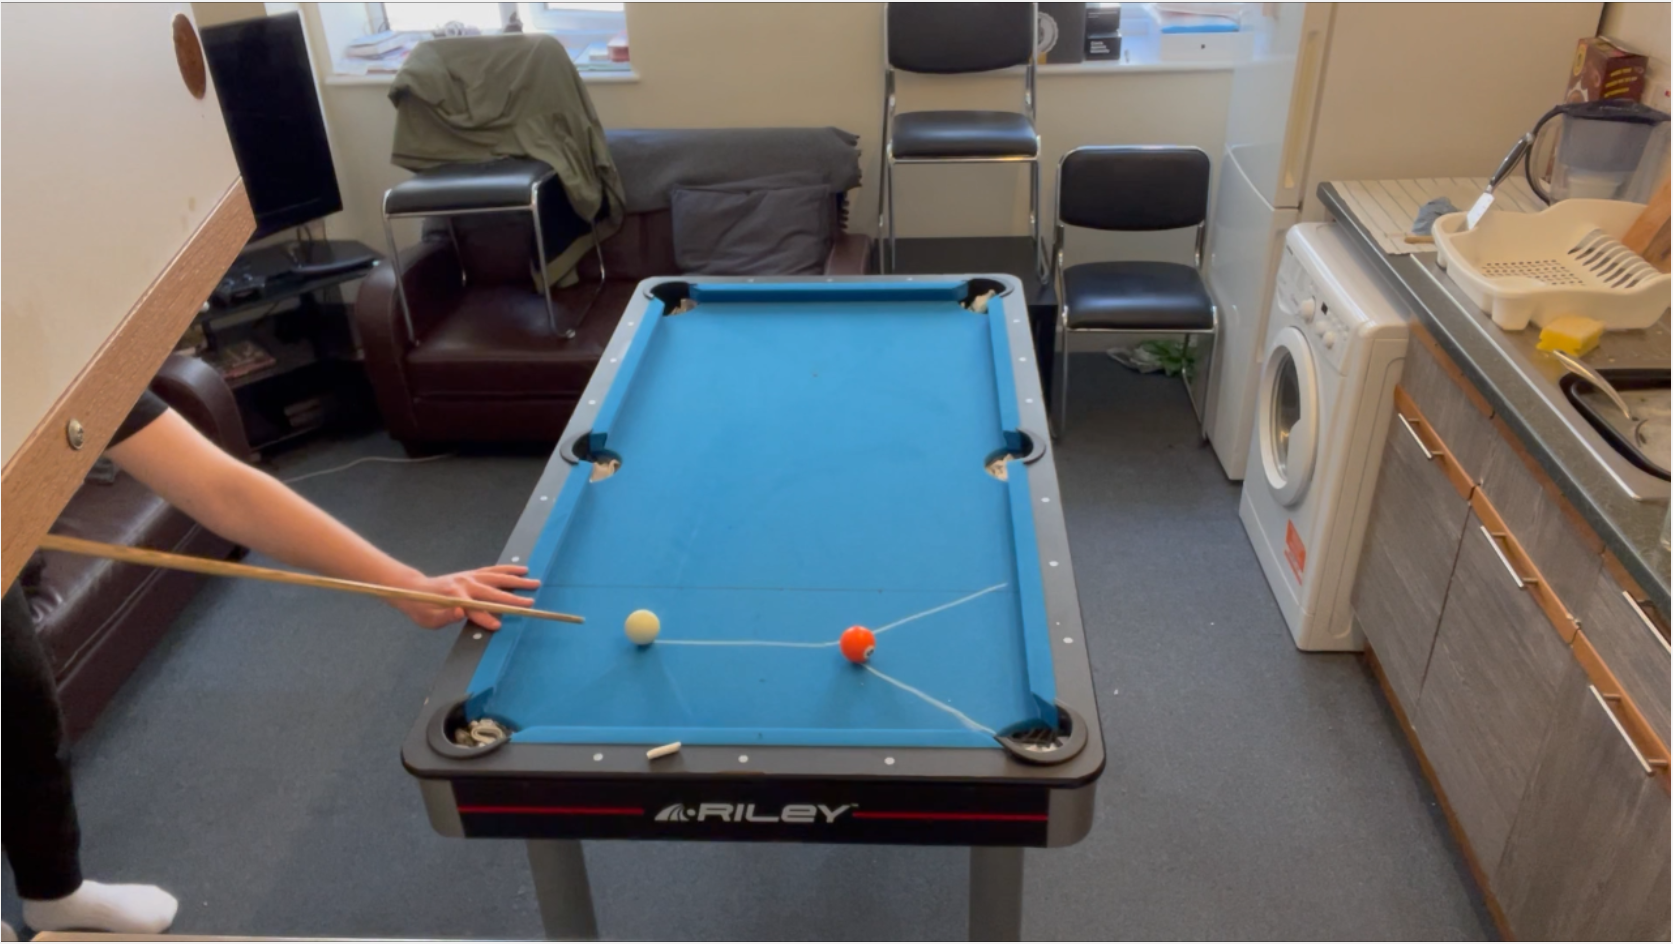
\includegraphics[scale = 0.15]{Images/Eval/Path Estimate/Cut Back/Frame 1.PNG} & 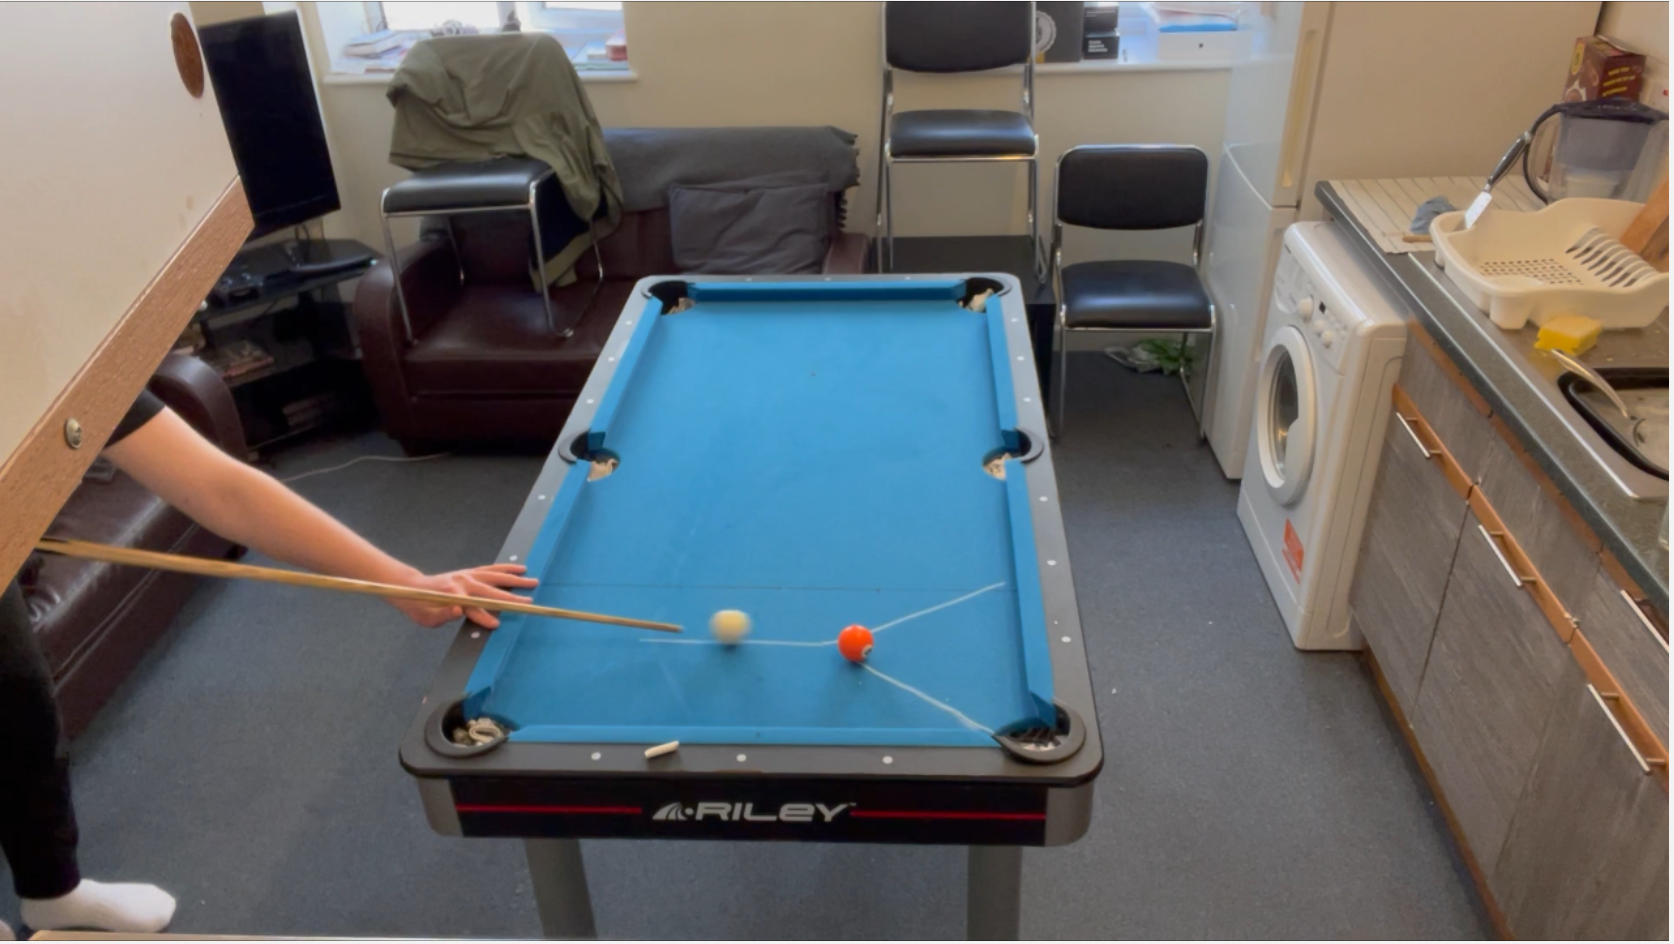
\includegraphics[scale = 0.15]{Images/Eval/Path Estimate/Cut Back/Frame 3.PNG} \\
         (a) Frame 1. & (b) Frame 3. \\ [6pt]
         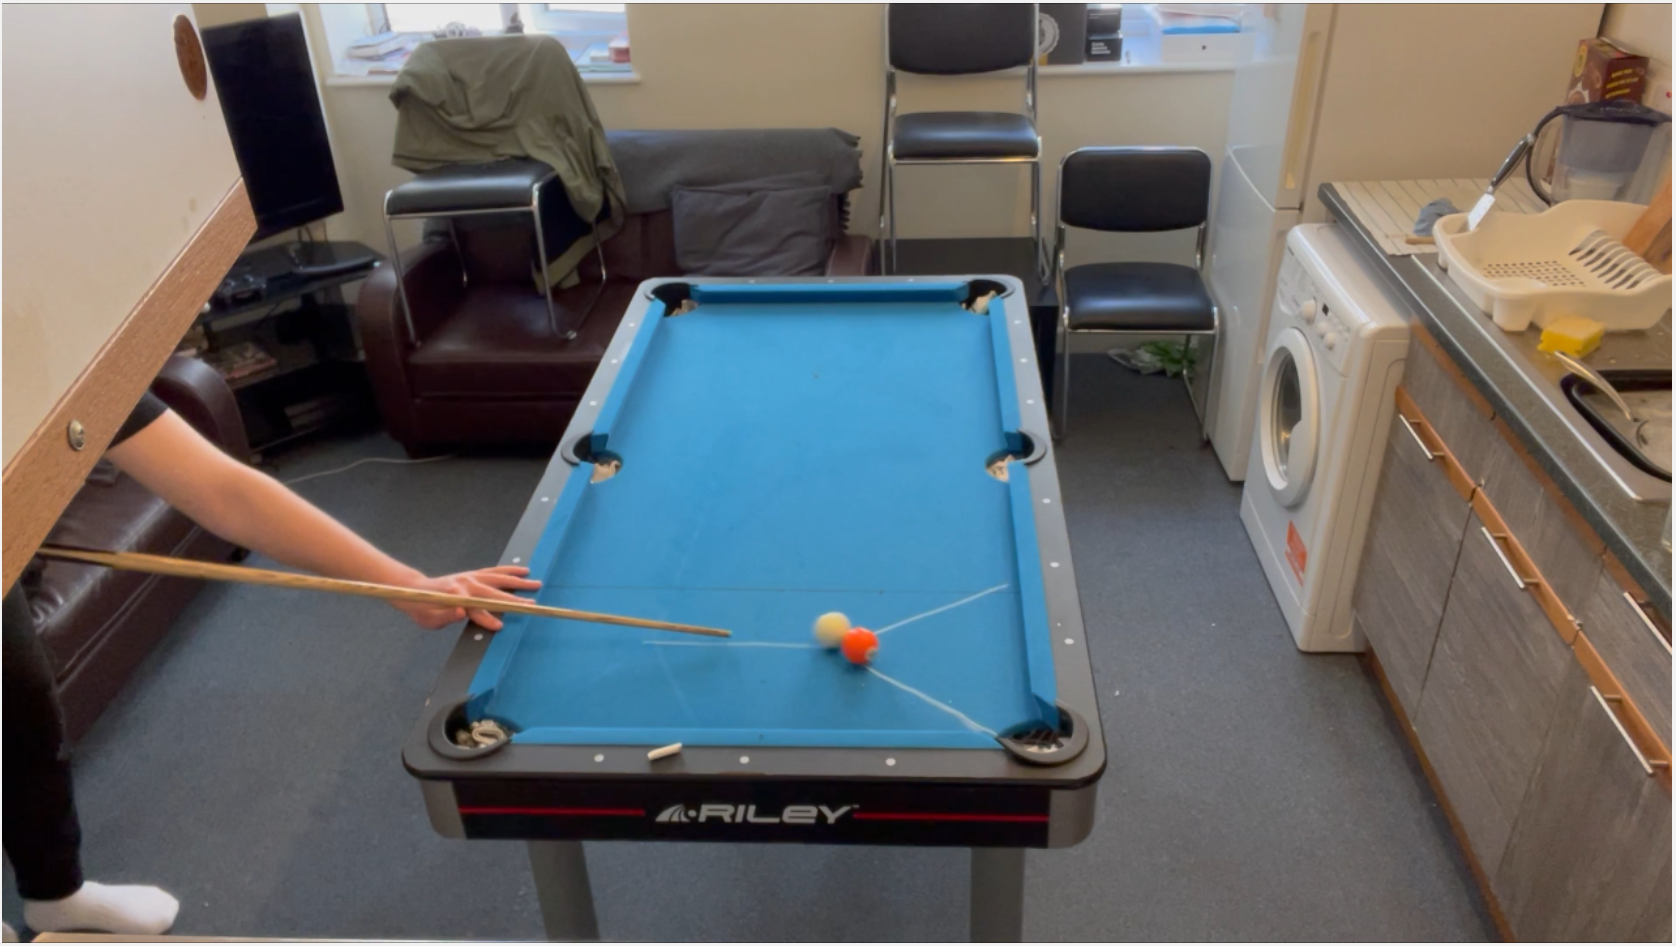
\includegraphics[scale = 0.15]{Images/Eval/Path Estimate/Cut Back/Frame 5.PNG} & 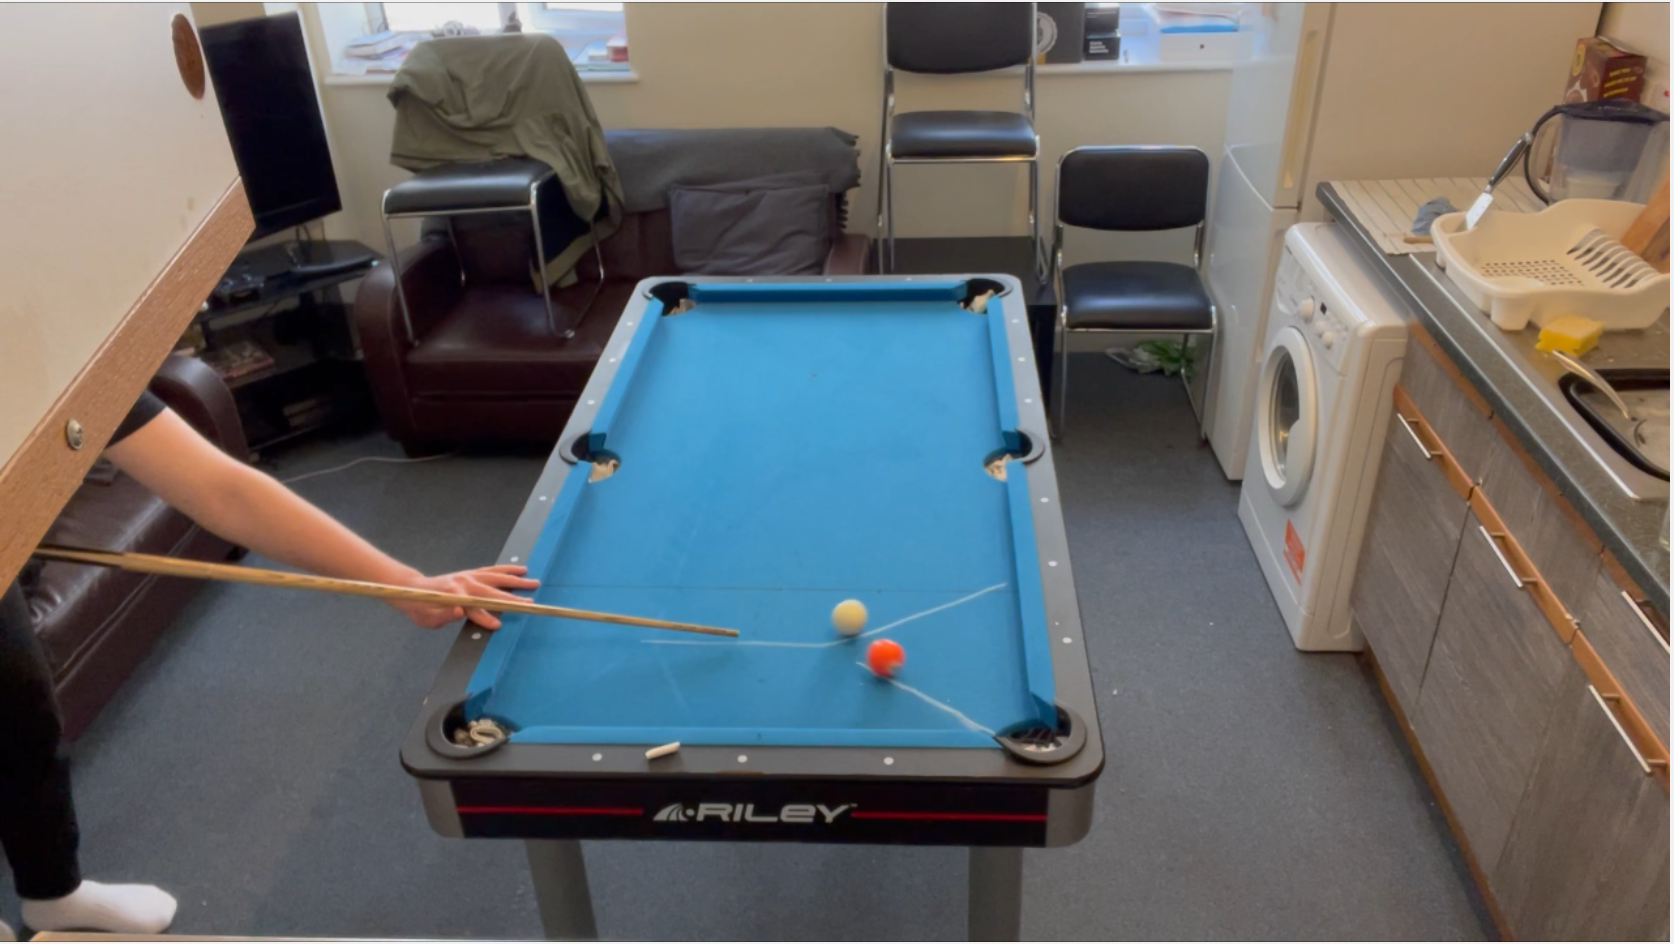
\includegraphics[scale = 0.15]{Images/Eval/Path Estimate/Cut Back/Frame 6.PNG} \\ 
         (c) Frame 5. & (d) Frame 6. \\ [6pt]
         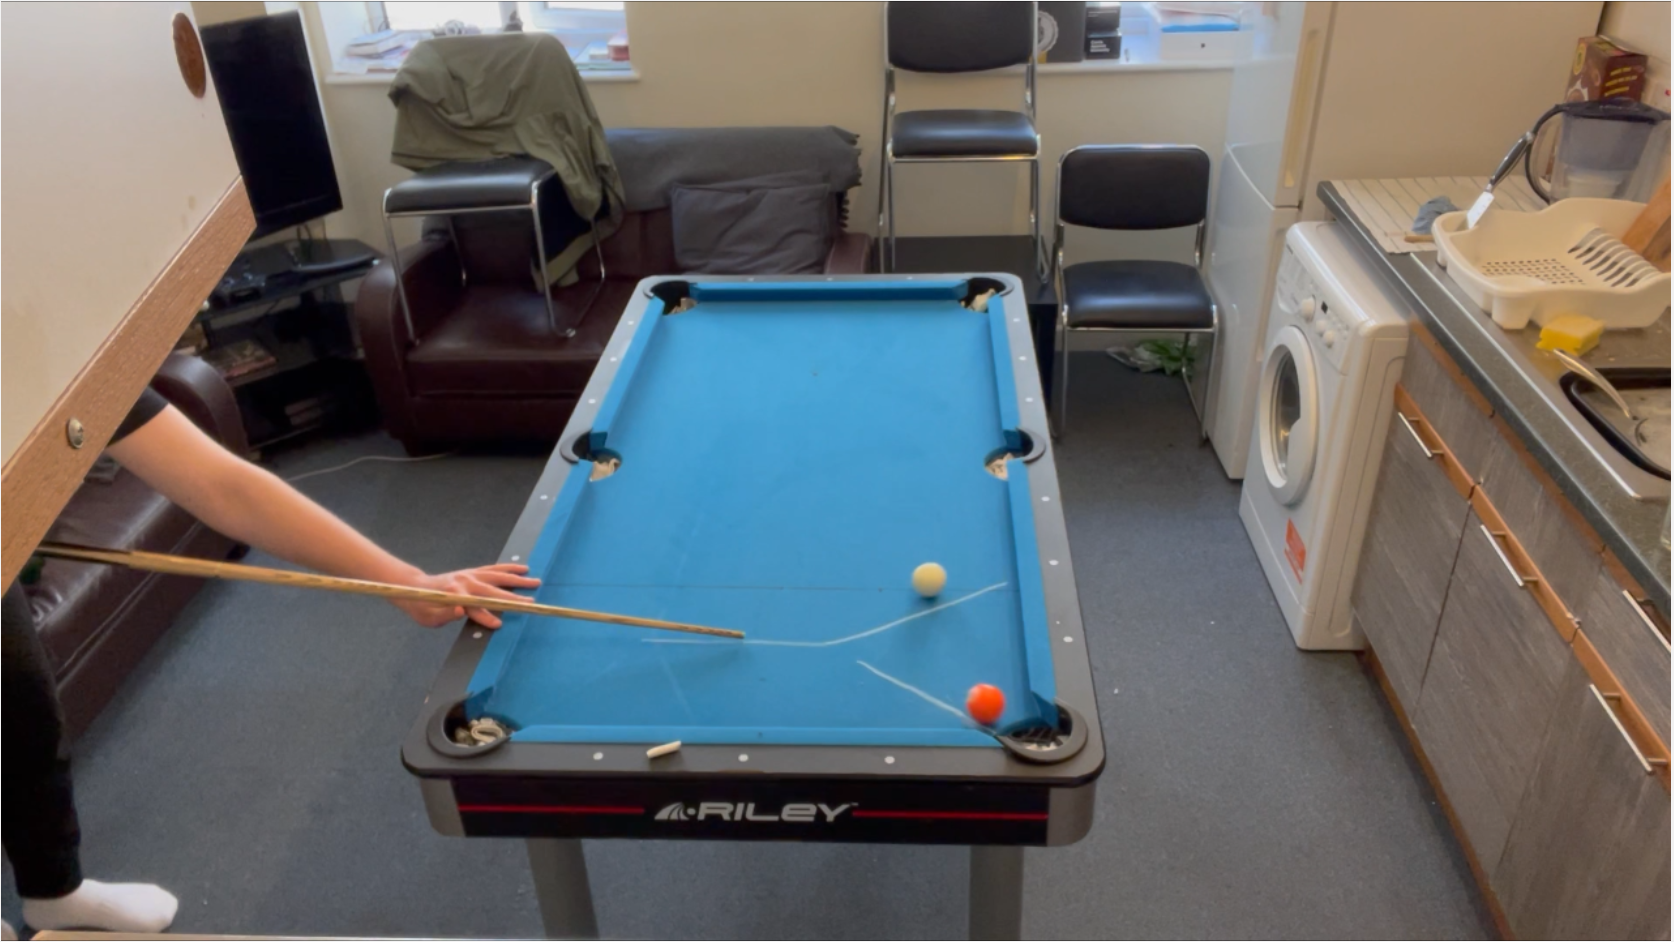
\includegraphics[scale = 0.15]{Images/Eval/Path Estimate/Cut Back/Frame 8.PNG} & 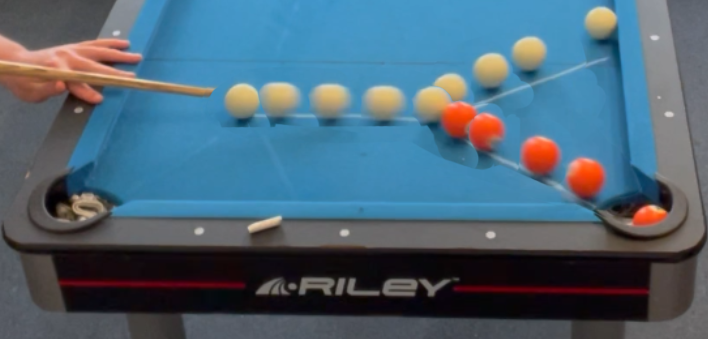
\includegraphics[scale = 0.15]{Images/Eval/Path Estimate/Cut Back/shot composition.png} \\
         (e) Frame 8. & (f) Superimposition of all frames from shot video.\\
    \end{tabular}
    \caption{Shown above are selected frames from the video taken of a cut-back shot to show the path taken by both balls. Image (f) are all 9 video frames superimposed to show the full trajectory of the ball.}
    \label{fig:evalCutBackShot}
\end{figure}

\begin{figure}[h!]
    \centering
    \begin{tabular}{cc}
         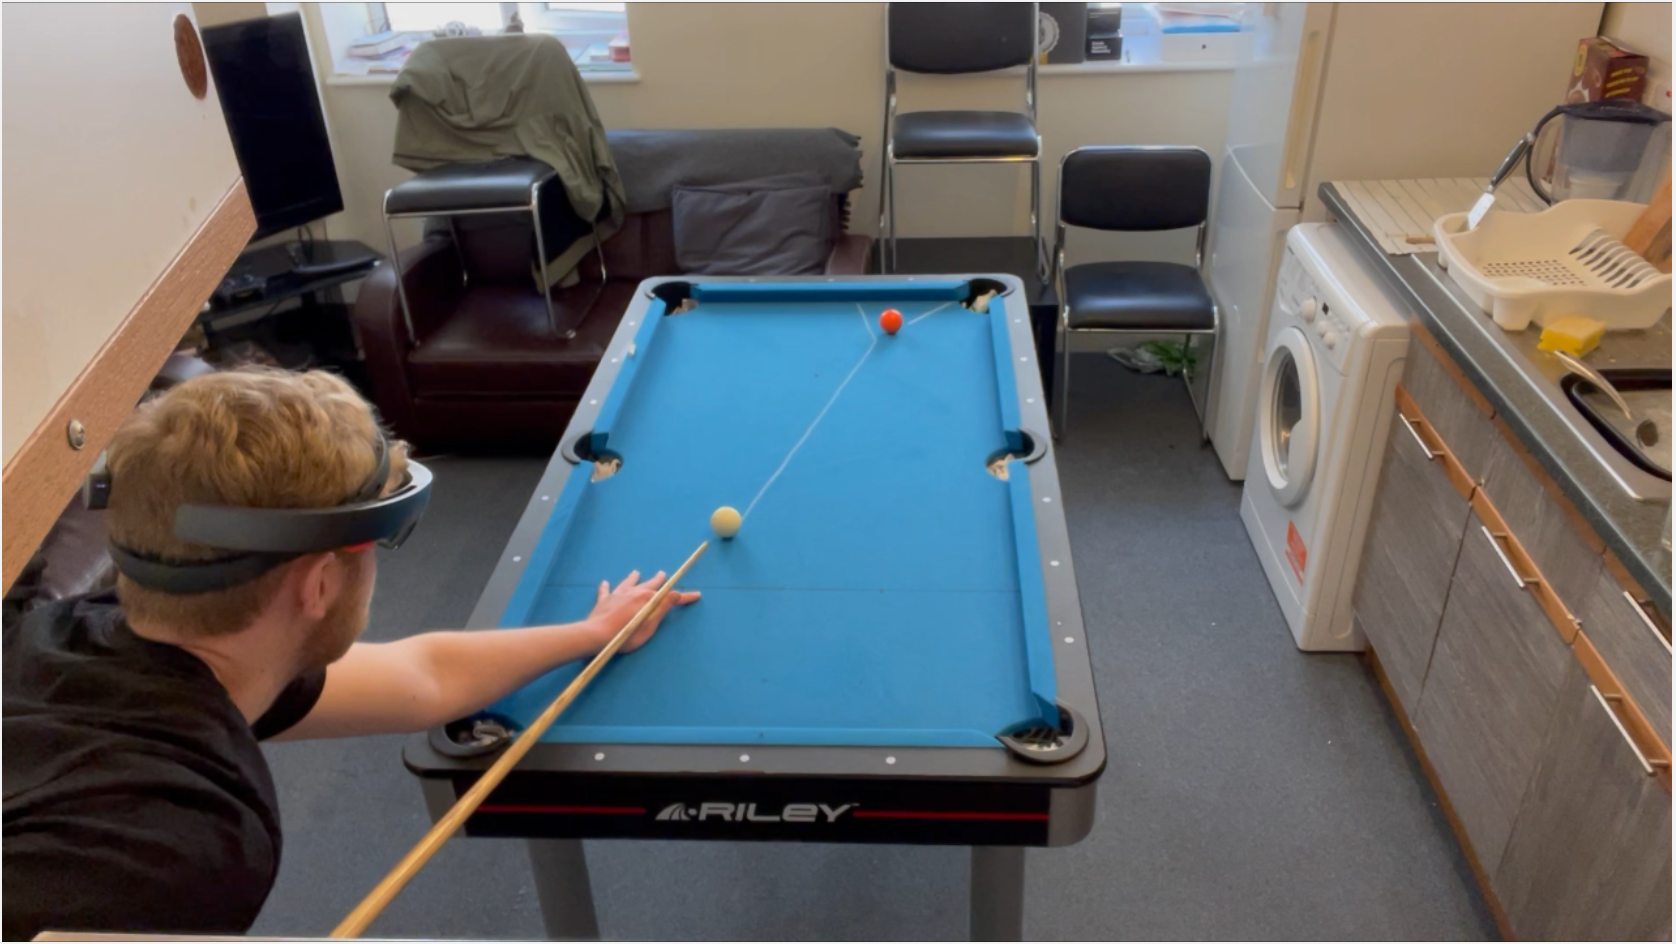
\includegraphics[scale = 0.15]{Images/Eval/Path Estimate/Cross Table/Frame 1.PNG} & 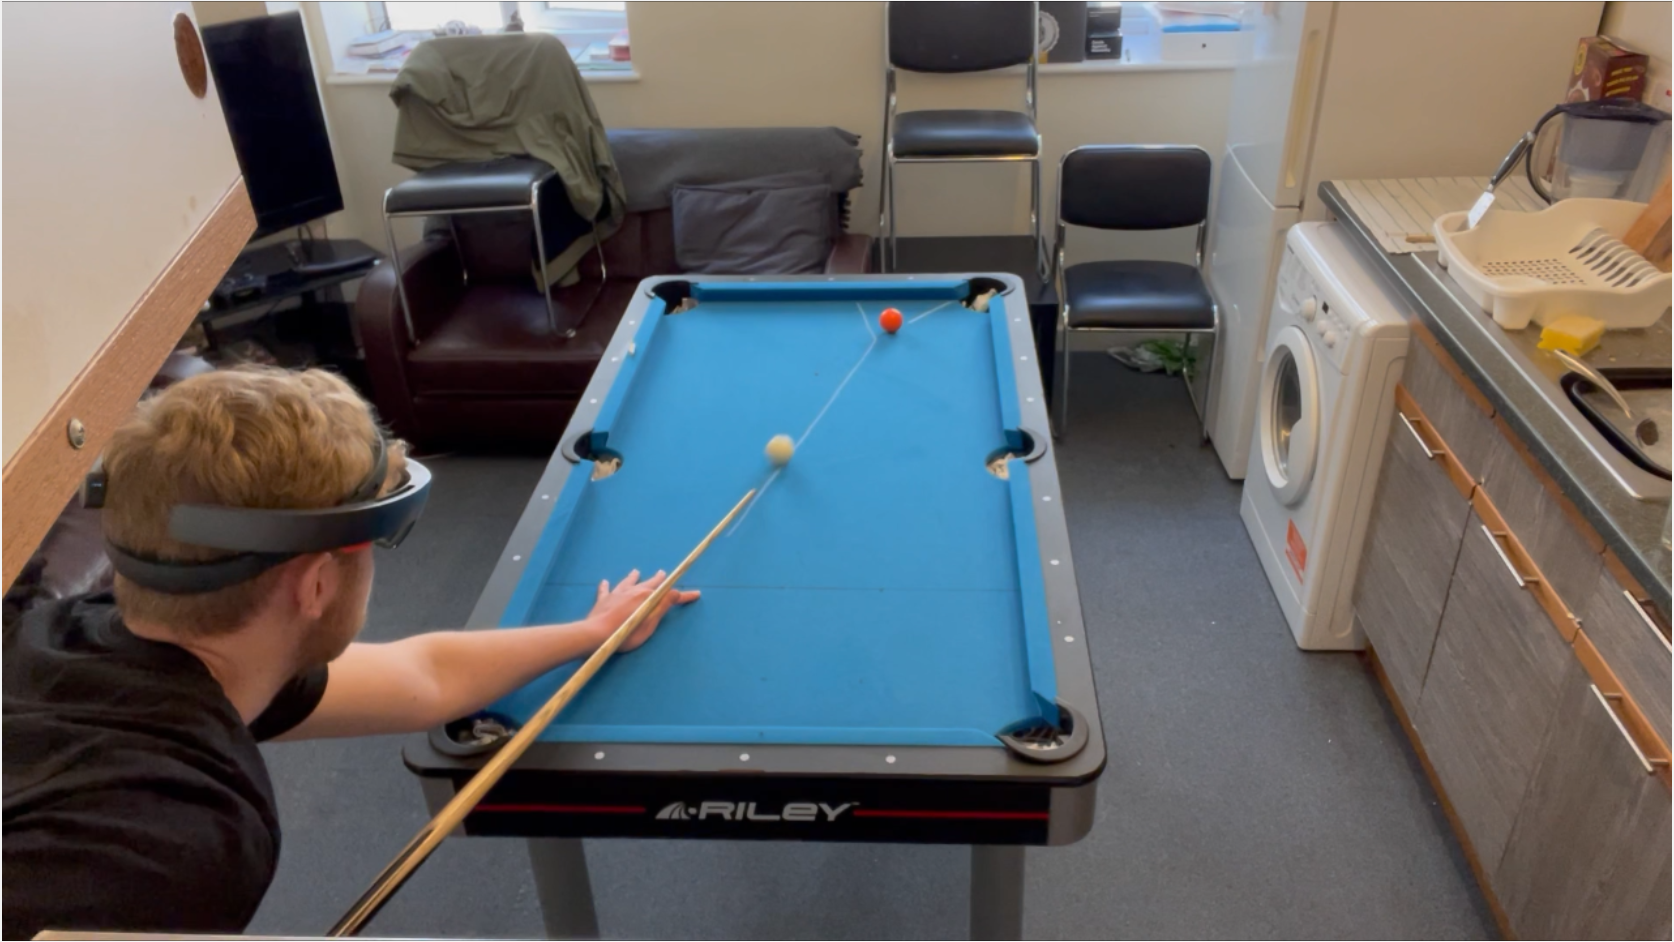
\includegraphics[scale = 0.15]{Images/Eval/Path Estimate/Cross Table/Frame 3.PNG} \\
         (a) Frame 1. & (b) Frame 3. \\ [6pt]
         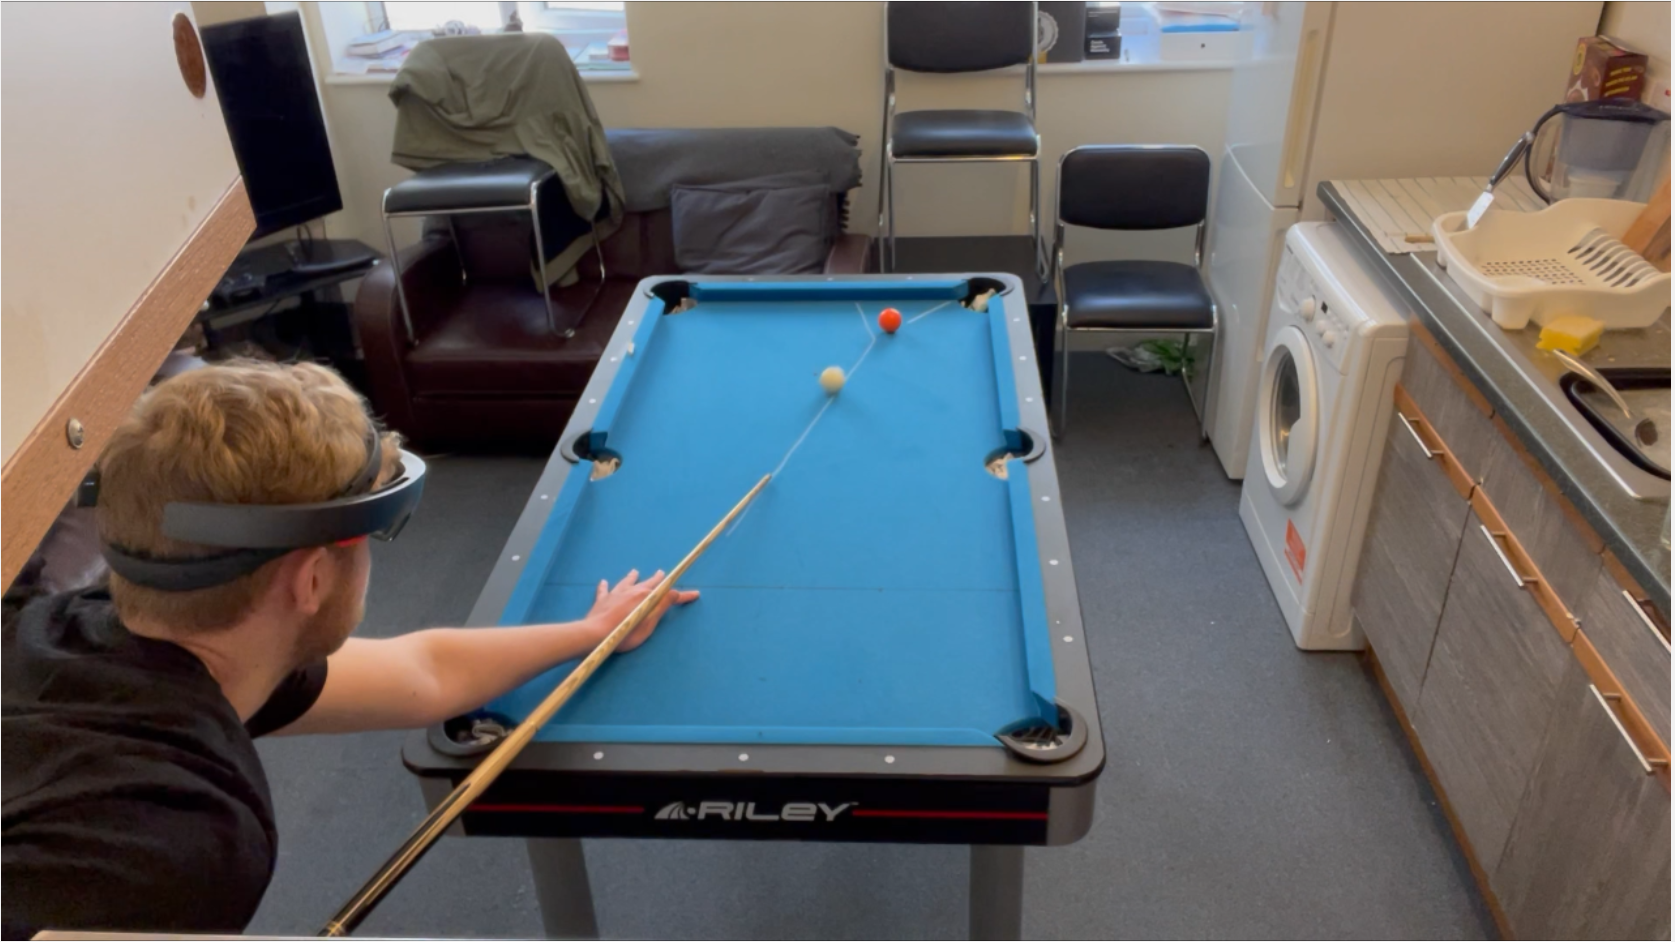
\includegraphics[scale = 0.15]{Images/Eval/Path Estimate/Cross Table/Frame 5.PNG} & 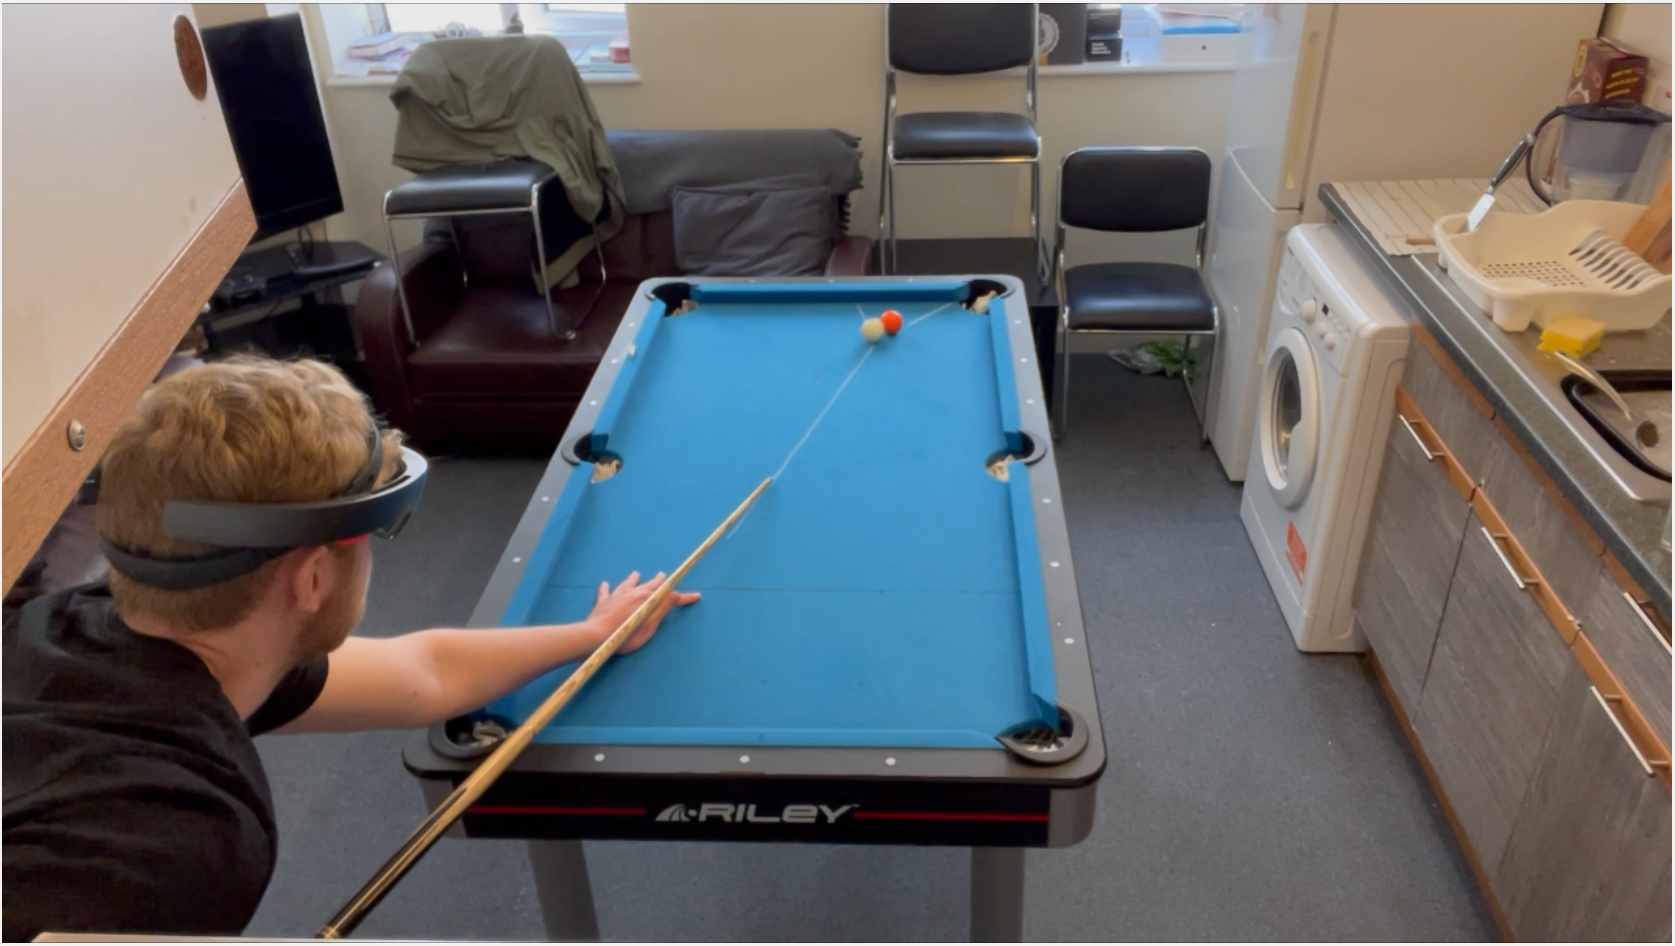
\includegraphics[scale = 0.15]{Images/Eval/Path Estimate/Cross Table/Frame 7.PNG}\\ 
         (c) Frame 5. & (d) Frame 7. \\ [6pt]
         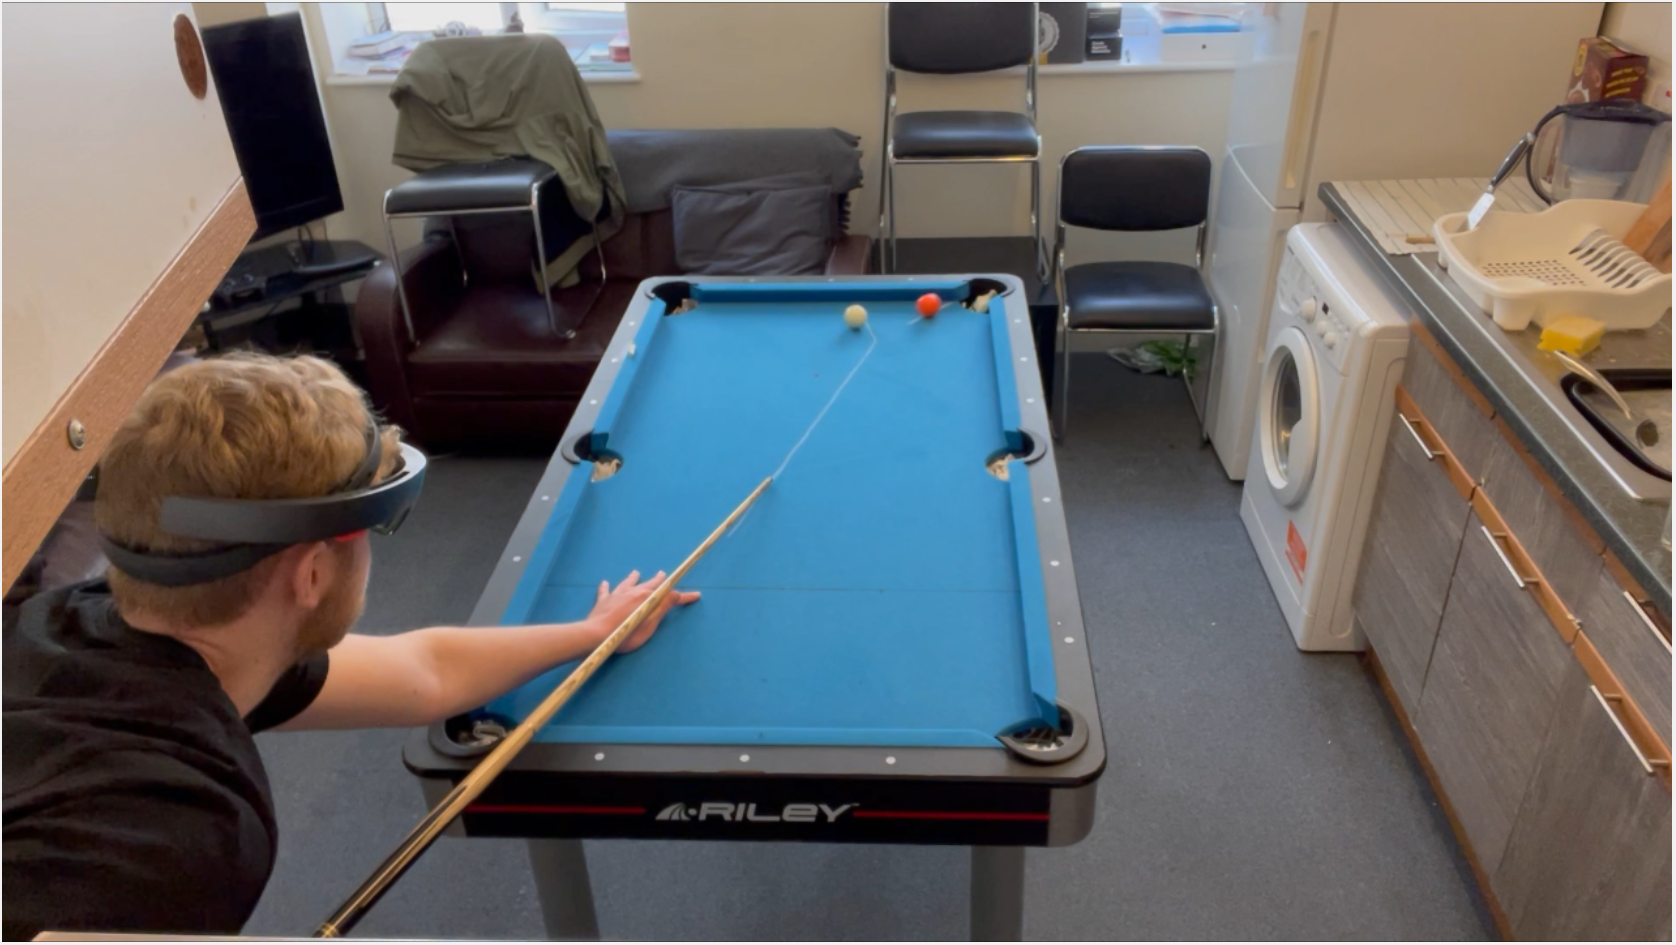
\includegraphics[scale = 0.15]{Images/Eval/Path Estimate/Cross Table/Frame 9.PNG} & 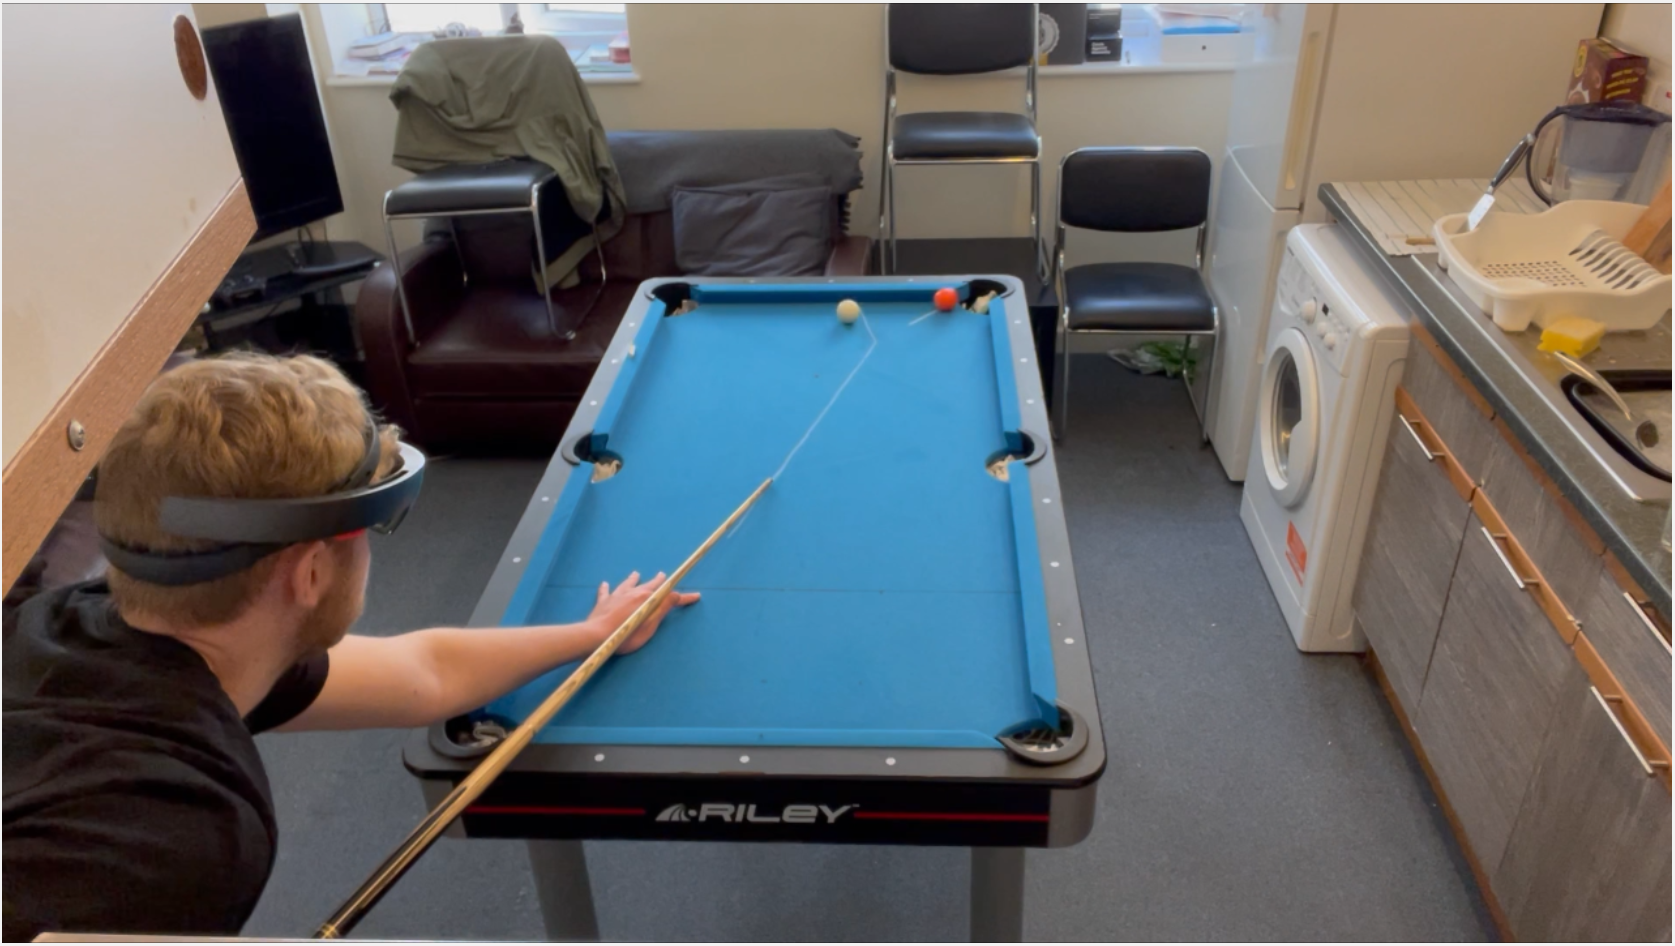
\includegraphics[scale = 0.15]{Images/Eval/Path Estimate/Cross Table/Frame 10.PNG}\\
         (e) Frame 9. & (f) Frame 10.\\
    \end{tabular}
    \caption{Shown above are selected frames from the video taken of a cross table shot to show the path taken by the cue ball and orange object ball.}
    \label{fig:evalCrossTableShot}
\end{figure}

\begin{figure}[h!]
    \centering
    \begin{tabular}{cc}
         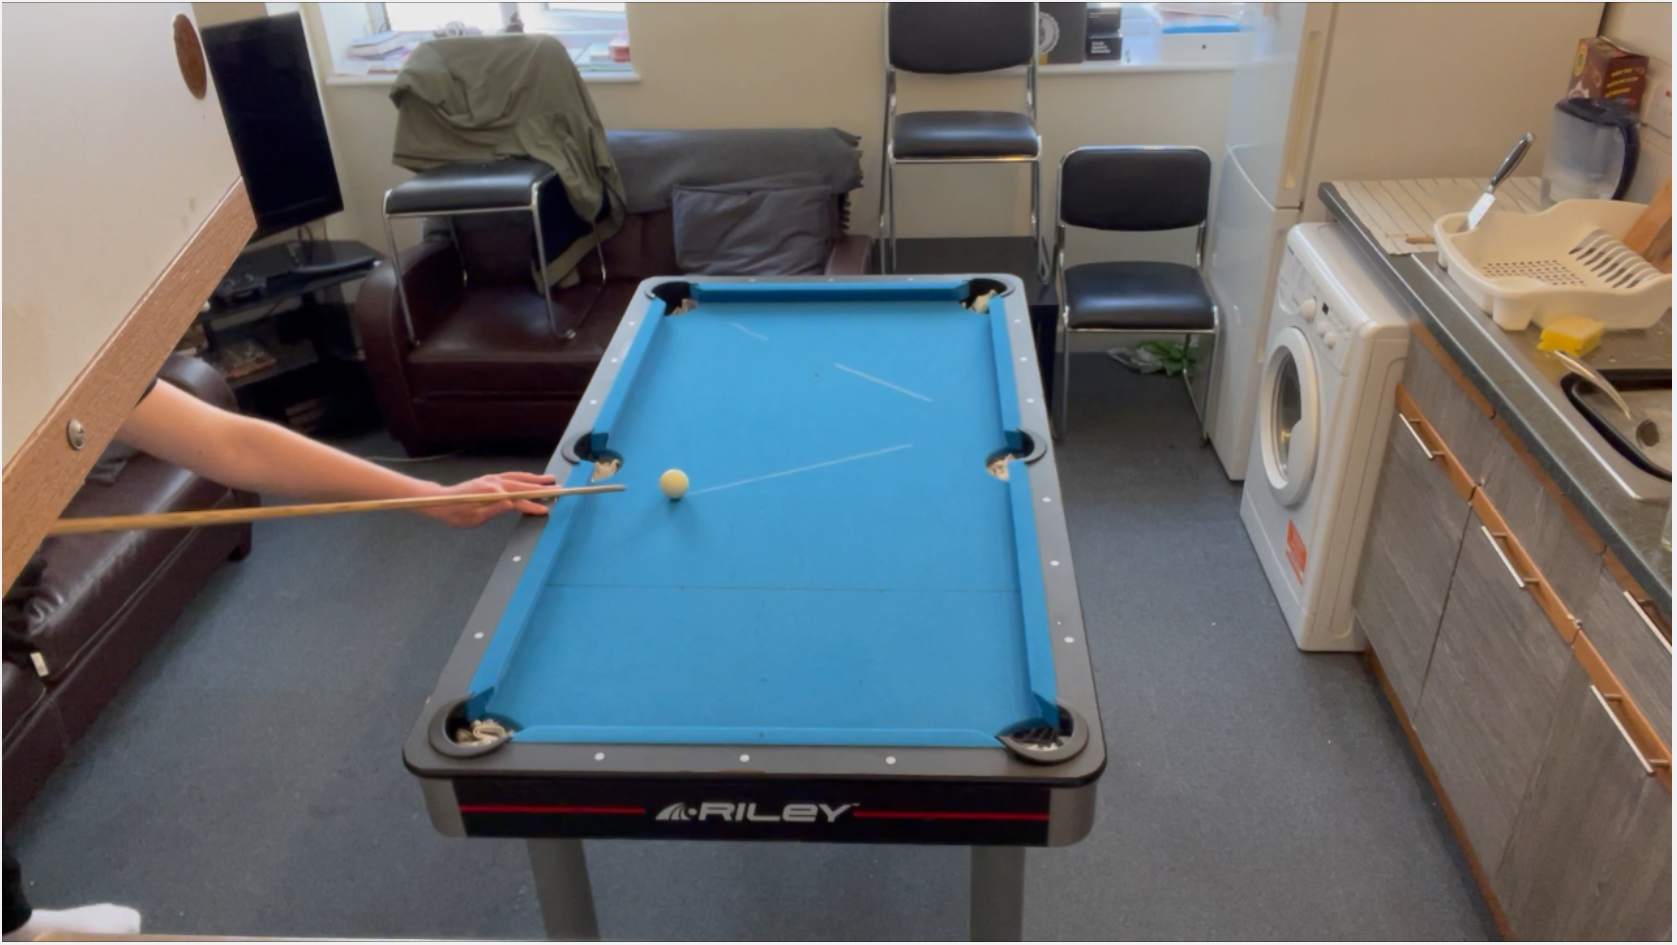
\includegraphics[scale = 0.15]{Images/Eval/Path Estimate/Rebound 2 Slow/Frame 1 - Shot 2 - Rebound 1.PNG} & 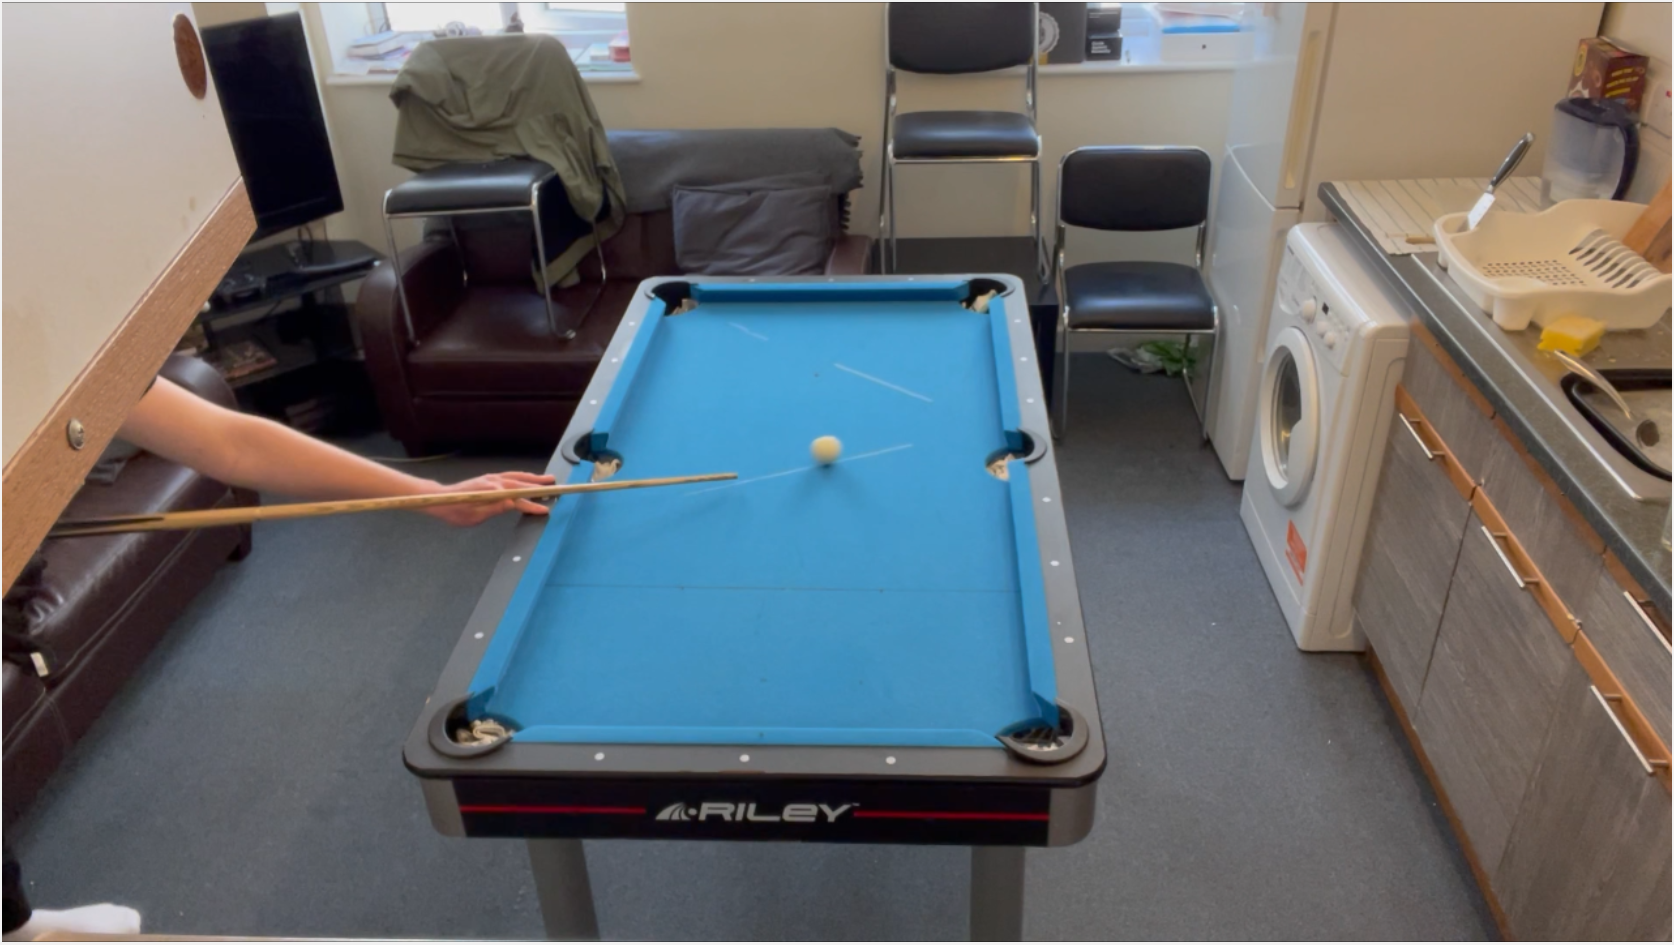
\includegraphics[scale = 0.15]{Images/Eval/Path Estimate/Rebound 2 Slow/Frame 4 - Shot 2 - Rebound 4.PNG} \\
         (a) Frame 1. & (b) Frame 4. \\ [6pt]
         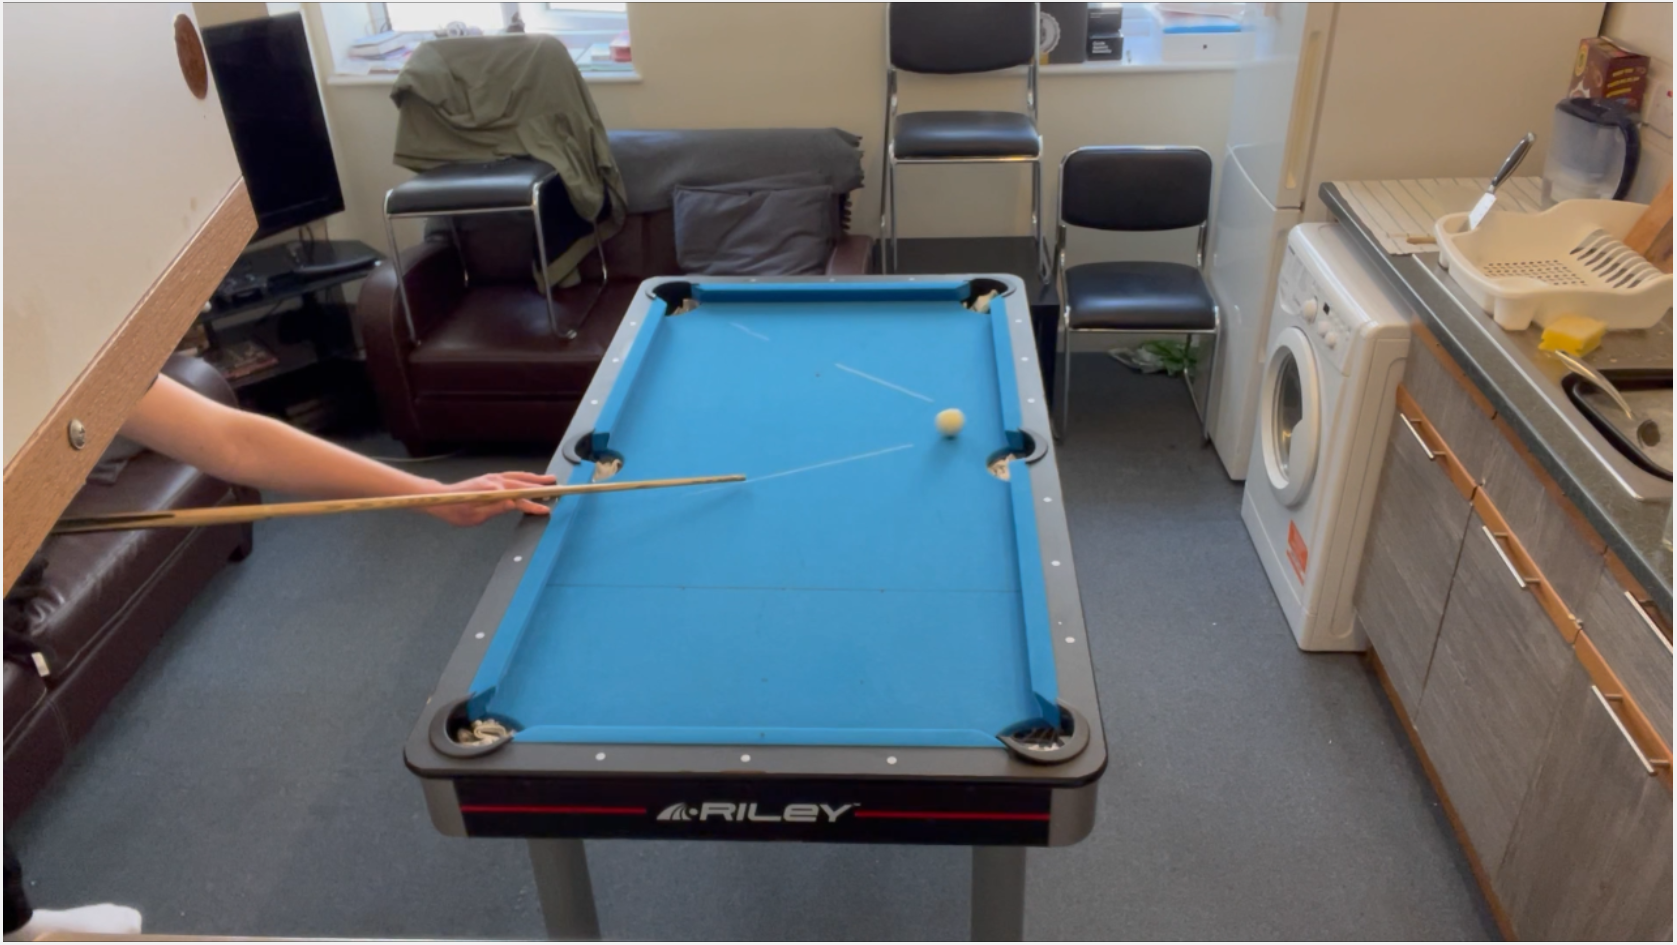
\includegraphics[scale = 0.15]{Images/Eval/Path Estimate/Rebound 2 Slow/Frame 6 - Shot 2 - Rebound 6.PNG} & 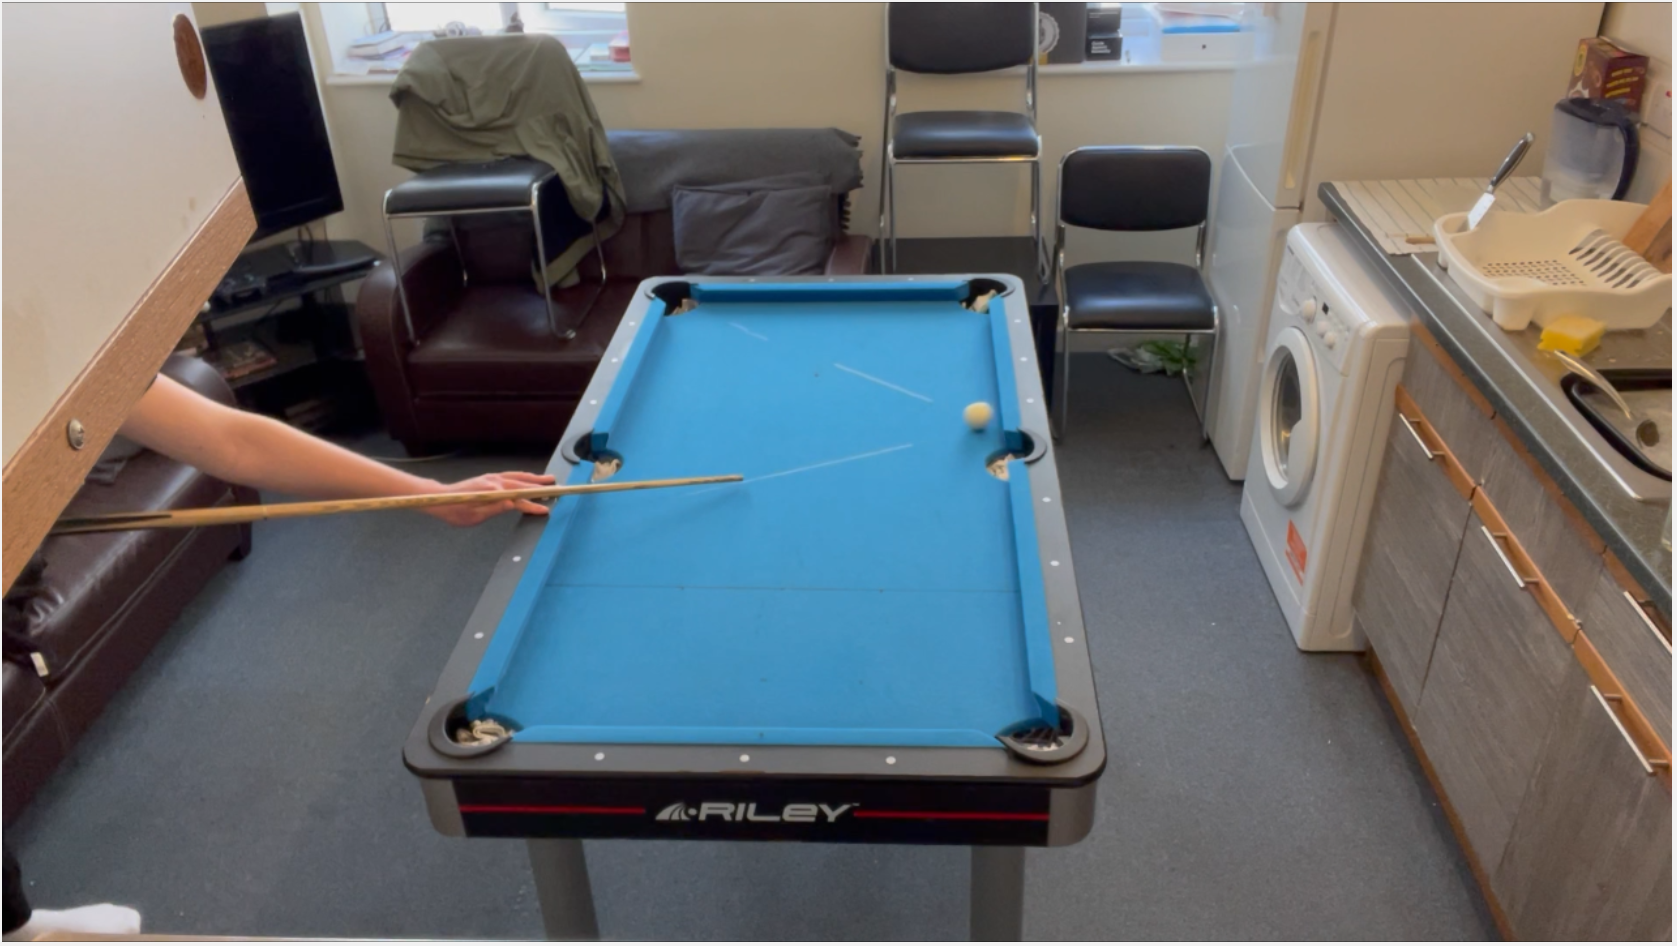
\includegraphics[scale = 0.15]{Images/Eval/Path Estimate/Rebound 2 Slow/Frame 7 - Shot 2 - Rebound 7.PNG}\\ 
         (c) Frame 6. & (d) Frame 7. \\ [6pt]
         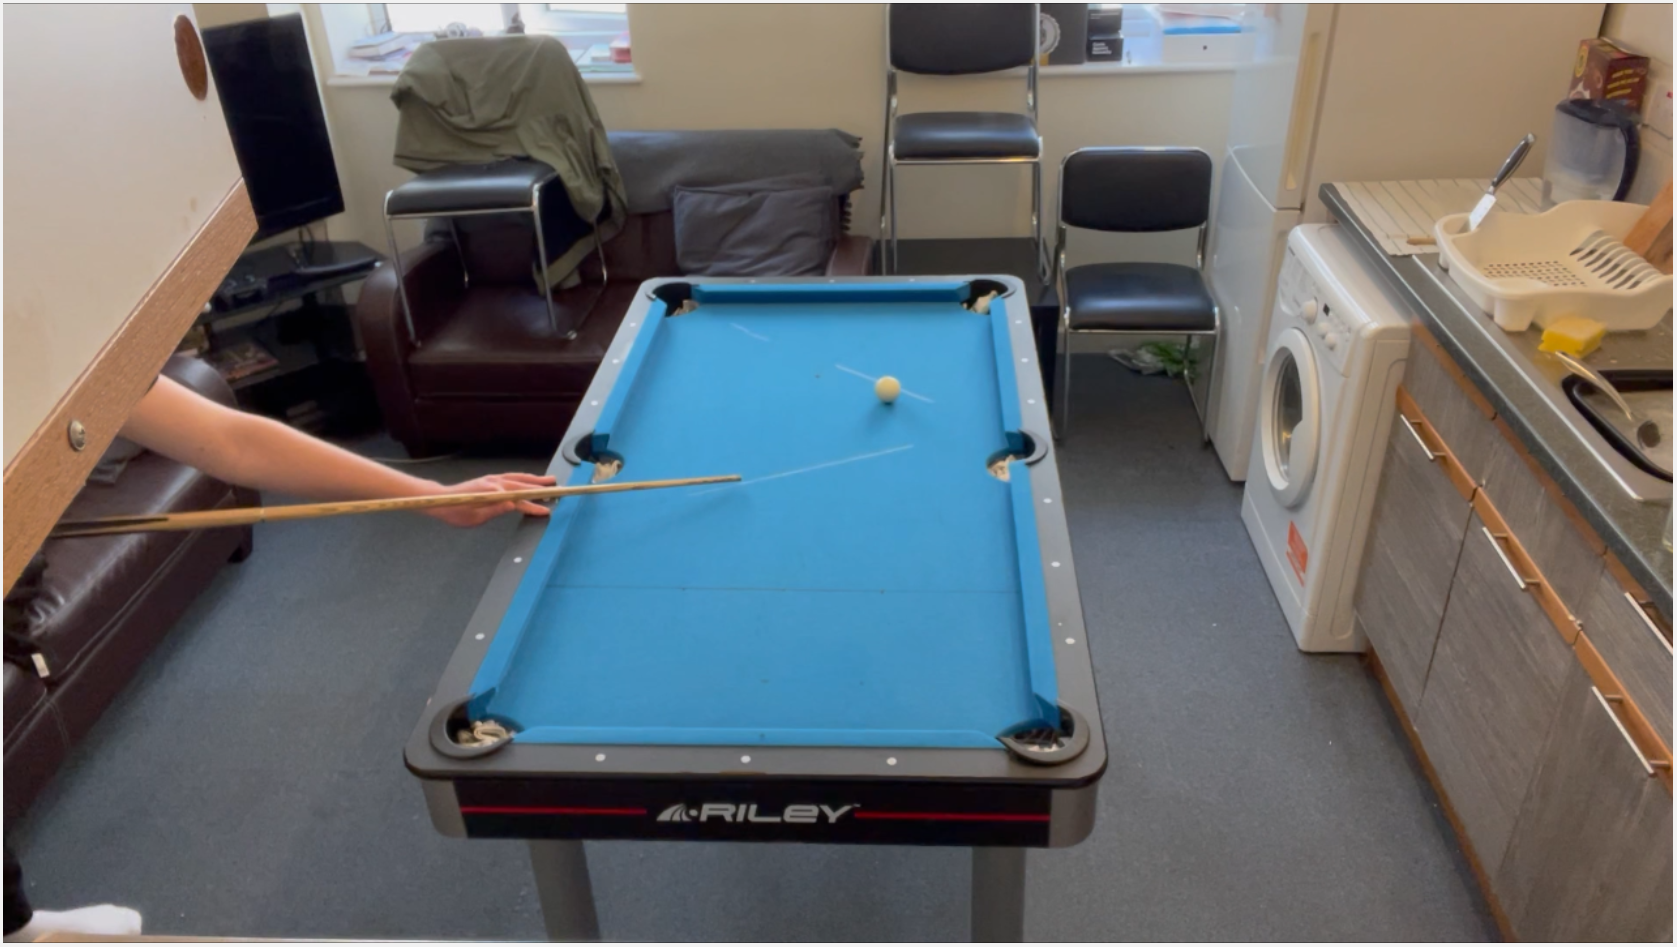
\includegraphics[scale = 0.15]{Images/Eval/Path Estimate/Rebound 2 Slow/Frame 11 - Shot 2 - Rebound 11.PNG} & 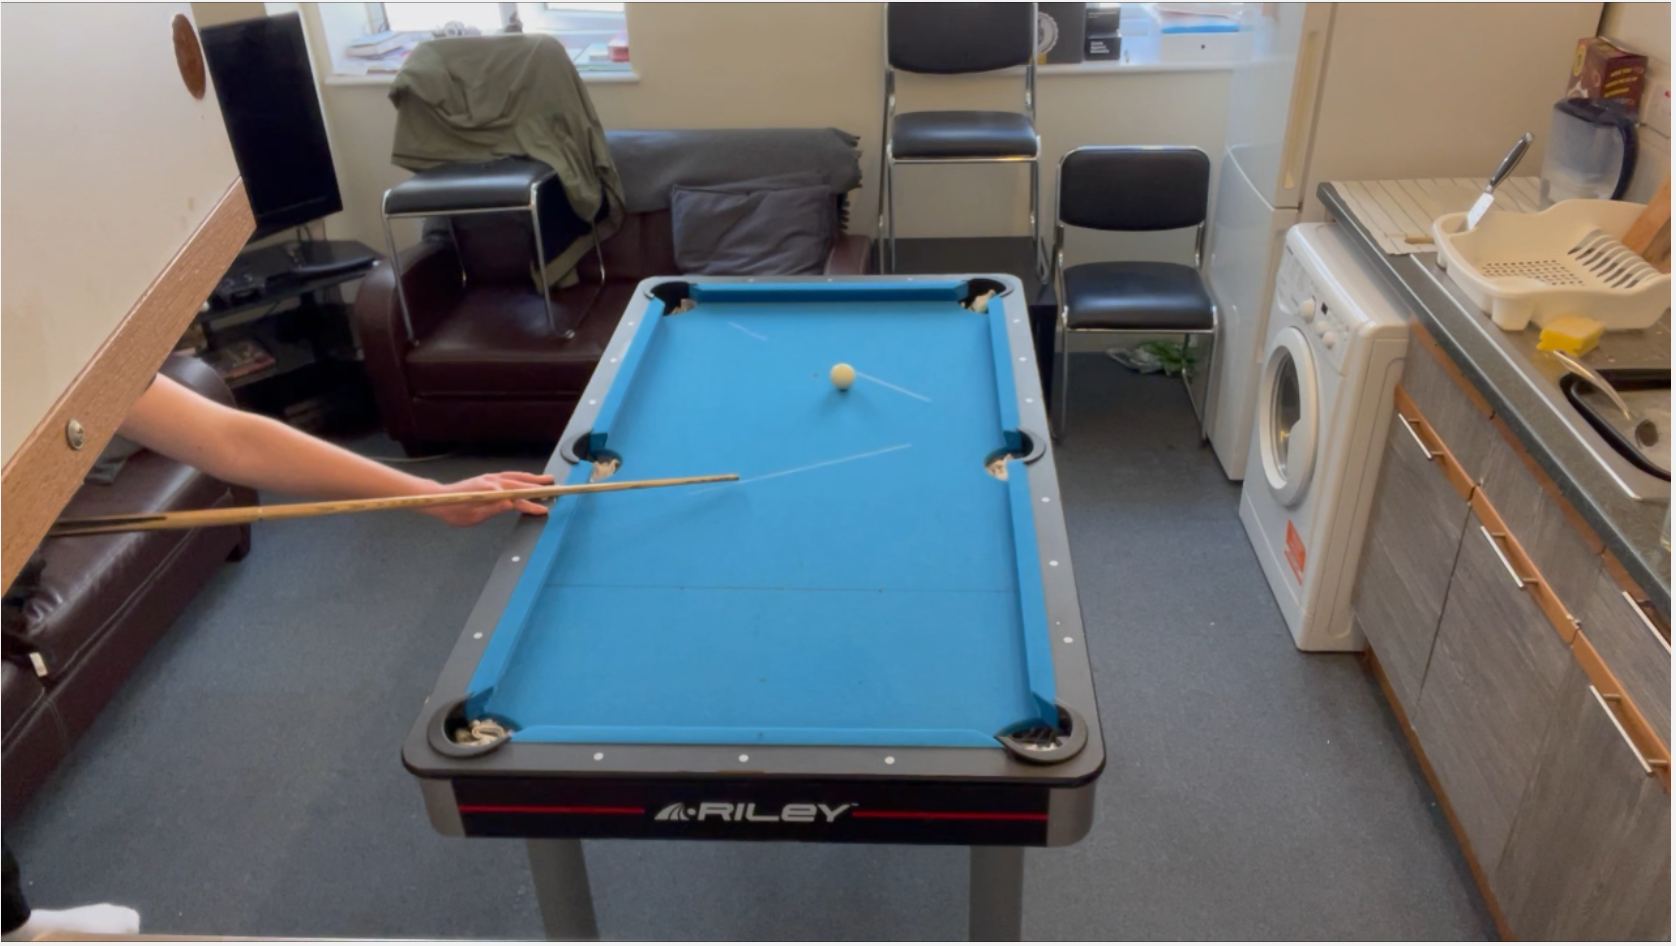
\includegraphics[scale = 0.15]{Images/Eval/Path Estimate/Rebound 2 Slow/Frame 12 - Shot 2 - Rebound 12.PNG}\\
         (e) Frame 11. & (f) Frame 12.\\
    \end{tabular}
    \caption{Shown above are selected frames from the video taken of a rebound shot to show the path taken by the cue ball.}
    \label{fig:evalReboundShot}
\end{figure}
 
\newpage

\section{User Shot Accuracy Improvement}
\label{eval:accuracyImprovement}
Addressing arguably the most important project objective, in person user testing was performed in order to assess if the application actually improves a user's potting accuracy, and to what degree\footnote{It is worth noting that due to the COVID-19 outbreak and subsequent social distancing precautions present at the time, only a few people were able to test the application safely whilst abiding to the government restrictions. Because of this, no substantial statistical analysis could be performed due to the small sample size, but, we can still evaluate any results that were collected and determine trends within the data.}. Each test user took a total of 7 pre-determined shots, such as the one shown in Figure \ref{fig:evalShot1}, both with the HoloLens headset using my application and without any additional aid. The shots were designed to replicate some of the most common shots someone would play in an ordinary game of pool or snooker whilst also varying in difficulty level. The full list of the shots performed is as follows; visual representations can be found in Appendix \ref{appx:shotDiagrams}.
\begin{itemize}
    \item \textbf{Shot 1 -} A cross table long shot.
    \item \textbf{Shot 2 -} A half table thin cut shot into the centre pocket.
    \item \textbf{Shot 3 -} A single rebound off of a cushion into a ball to pot it.
    \item \textbf{Shot 4 -} A double rebound off of two cushions into a ball to pot it.
    \item \textbf{Shot 5 -} A cross table long shot where other balls must be avoided.
    \item \textbf{Shot 6 -} A cross table long shot, but with the object ball placed just in-front of the cue ball.
    \item \textbf{Shot 7 -} A cut back shot.
\end{itemize}

In order to try and mitigate any learning effect the user could experience just from playing pool (i.e. their accuracy improves throughout the test only due to them playing), half of the test users took the shots with my system first then without, while the other half did the opposite. \\\par

\begin{figure}[h!]
    \centering
    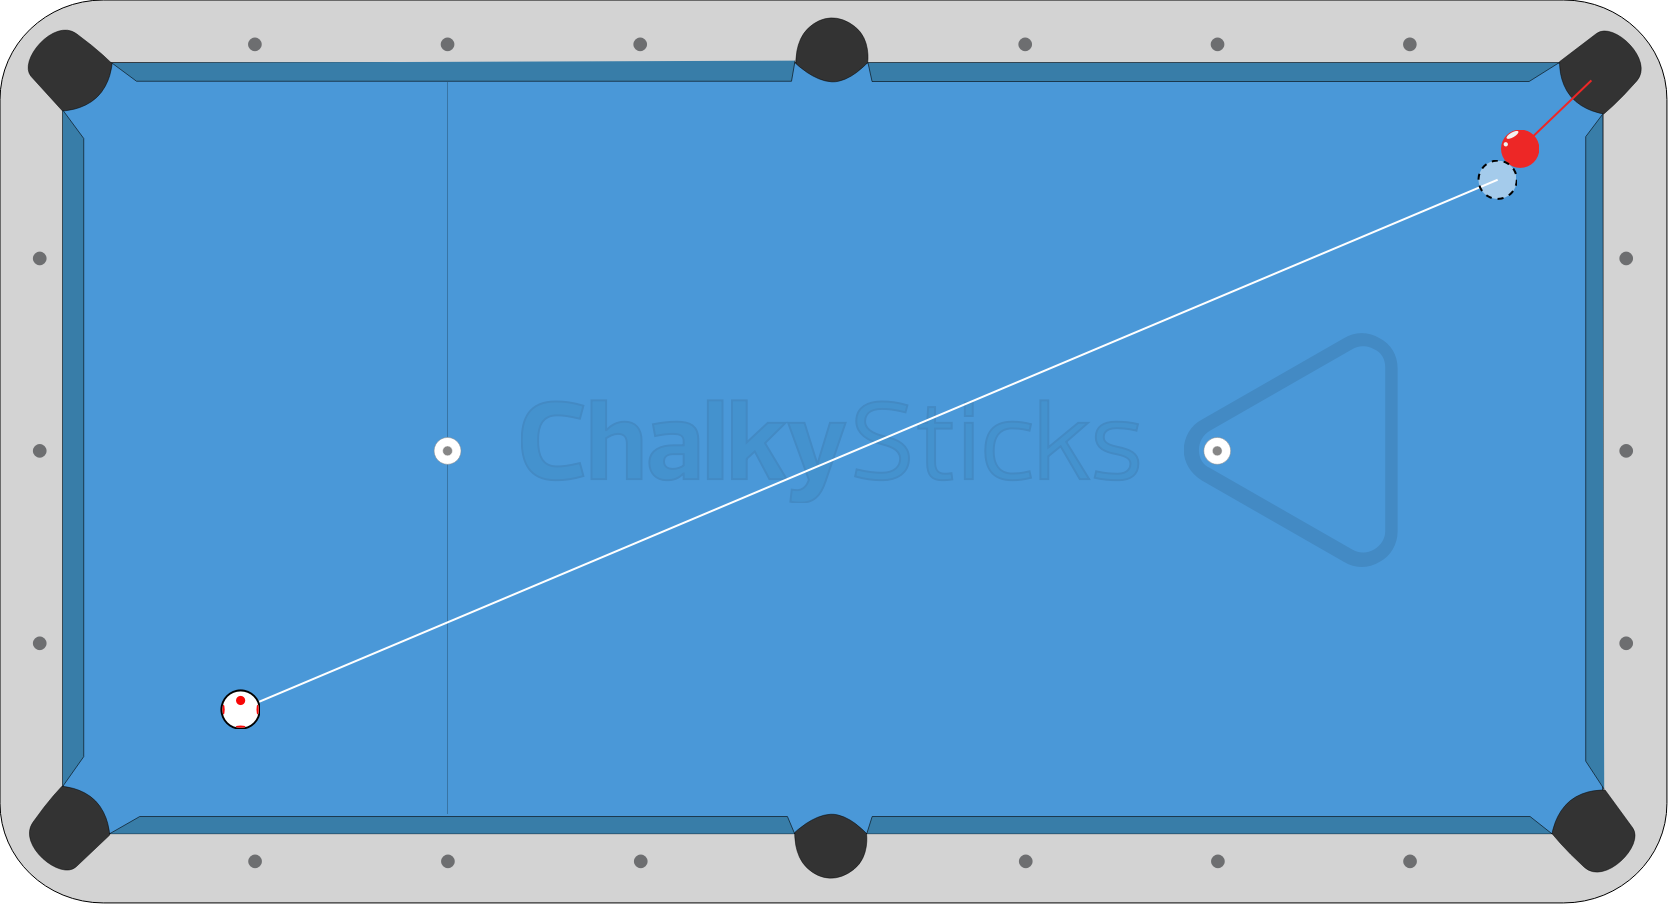
\includegraphics[scale = 0.15]{Images/Shot Diagrams/Shot_1.png}
    \caption{Shot 1 - An across table long shot. Graphic created using Chalky Sticks \cite{chalkySticks}.}
    \label{fig:evalShot1}
\end{figure}

In total, four people tested my application, of whom two thought of their skill level as beginner (Users 3 and 4) and two thought of their skill level as intermediate (Users 1 and 2). It was ensured that one player from each skill level played the seven shots with my aiming assistant first, and one player from each skill level played the seven shots without my aiming assistant first. For each of the seven shots, the user was told which ball to target, which pocket to aim for, and which cushions to hit (if appropriate to the shot). A successful pot was recorded if all of the aforementioned shot conditions were met, otherwise, the shot was considered unsuccessful. Prior to taking the shots with the HoloLens on, each test user completed the \textit{Learn Gestures} application that comes pre-loaded on the HoloLens\cite{learnGestures} to ensure that they were able to get to grips with how to correctly interact with the device. A full breakdown of all of the test user's results can be found below in Table \ref{tab:userResultsIntermediate} and Table \ref{tab:userResultsBeginner}. \\

\begin{table}[h!]
    \centering
    \begin{tabular}{|c||c|c||c|c|}
        \hline
        & \multicolumn{2}{c||}{User 1} & \multicolumn{2}{c|}{User 2}\\
        \hline
        & With Headset & Without Headset & With Headset & Without Headset\\
        \hline
        Shot \ref{fig:shot1} & X & \checkmark & \checkmark & \checkmark \\
        \hline
        Shot \ref{fig:shot2} & \checkmark & \checkmark & X & \checkmark \\
        \hline
        Shot \ref{fig:shot3} & X & X & X & \checkmark \\
        \hline
        Shot \ref{fig:shot4} & X & X & X & X \\
        \hline
        Shot \ref{fig:shot5} & \checkmark & \checkmark & \checkmark & \checkmark \\
        \hline
        Shot \ref{fig:shot6} & X & X & \checkmark & \checkmark \\
        \hline
        Shot \ref{fig:shot7} & X & X & X & X \\
        \hline
    \end{tabular}
    \caption{Results from the user accuracy test for both intermediate skill level users. A check mark indicates the shot was potted successfully, a cross indicates the shot was not potted successfully. Results from the user using my aim assistant application (indicated by the \textit{With Headset} column) and not using my application (indicated by the \textit{Without Headset} column) are presented.}
    \label{tab:userResultsIntermediate}
\end{table}

\begin{table}[h!]
    \centering
    \begin{tabular}{|c||c|c||c|c|}
        \hline
        & \multicolumn{2}{c||}{User 3} & \multicolumn{2}{c|}{User 4}\\
        \hline
        & With Headset & Without Headset & With Headset & Without Headset\\
        \hline
        Shot \ref{fig:shot1} & \checkmark & X & \checkmark & X \\
        \hline
        Shot \ref{fig:shot2} & \checkmark & X & X & X \\
        \hline
        Shot \ref{fig:shot3} & X & X & X & X \\
        \hline
        Shot \ref{fig:shot4} & X & X & X & X \\
        \hline
        Shot \ref{fig:shot5} & \checkmark & X & X & X \\
        \hline
        Shot \ref{fig:shot6} & \checkmark & \checkmark & \checkmark & \checkmark \\
        \hline
        Shot \ref{fig:shot7} & X & X & \checkmark & X \\
        \hline
    \end{tabular}
    \caption{Results from the user accuracy test for both beginner skill level users. A check mark indicates the shot was potted successfully, a cross indicates the shot was not potted successfully. Results from the user using my aim assistant application (indicated by the \textit{With Headset} column) and not using my application (indicated by the \textit{Without Headset} column) are presented.}
    \label{tab:userResultsBeginner}
\end{table}

It is worth analysing a few of the unsuccessful shots the intermediate users had whilst using my aim assistant from Table \ref{tab:userResultsIntermediate}. With User 1, they failed to pot Shot \ref{fig:shot1} with the headset on, but successfully potted it without using my aim assistant. At the time they explained \textit{"The cue ball seemed to follow the line exactly."} which could point us towards the assumption that the user miss-aligned one of the balls, the table, or simply aimed incorrectly. Additionally, this was the first shot that they played with my aim assistant and so they could have still been getting used to using it, however, given that the other three test users all potted Shot \ref{fig:shot1} whilst using my aim assistant, I think this is unlikely. Given a larger sample size, it would be interesting to see if this was a common theme throughout.\\

The two shots that User 2 failed to pot whilst using my aim assistant, but succeeded in potting when not using my aim assistant, were Shot \ref{fig:shot2} and Shot \ref{fig:shot3}; a very thin cut shot and a rebound shot respectively. Concerning Shot \ref{fig:shot2}, very precise aim is required in order to successfully make this shot. Given that all users commented on it being somewhat difficult to place the balls and table, as well as how sensitive the aiming marker was to move, we could attribute this unsuccessful pot to some minor misalignment. Further reinforcing this is the fact that overall, only two out of the four test users successfully potted Shot \ref{fig:shot2} whilst using my aim assistant, one from each skill level. The same conclusion of object misalignment could be made for Shot \ref{fig:shot7}, another difficult thin cut shot, with only one out of the four test users successfully potting this shot with or without the use of my aim assistant. Noting that this single successful pot for Shot \ref{fig:shot7} was completed whilst using my aim assistant, it shows that when set-up correctly, it can help a user make very difficult shots.\\

Moving onto Shot \ref{fig:shot3}. Being a rebound shot, it is notoriously difficult for even highly skill players to pot successfully. This is reflected in my results with only a single successful pot for either of the two rebound shots (Shot \ref{fig:shot3} and Shot \ref{fig:shot4}) attained from all test users. Given that from Section \ref{eval:pathAccuracy} above it was discussed that the calculation of post cushion collisions was somewhat inaccurate, and relies on many assumptions, this result is not too surprising. However, being able to hit rebound shots successfully is a highly important skill in getting out of snookered\footnote{A situation where the cue ball position is such that one cannot directly hit the required object ball.} positions, and so the fact that my aim assistant cannot currently provide accurate help in these situations is somewhat disappointing. \\

After all shots were taken, both intermediate players saw a drop in how many shots they potted when using the aim assistant compared to not using it. User 1 saw a 33\% drop, going from 3 pots to 2, whilst User 2 saw a 40\% drop, going from 5 pots to 3. All shots that were potted whilst using the headset were also potted without for both users. Conversely, for both beginner players an increase in potting success was seen when using my aim assistant compared to not using it. User 3 had an increase of 300\%, going from 1 successful pot without the headset to 4 successful pots with the headset, and User 4 had a 200\% increase in potting success, going from 1 successful pot without the headset to 3 successful pots with the headset. From these results we can see that my aim assistant application seems to benefits less skillful players much more than someone with previous playing experience. \\

One explanation of why the system benefits less skillful players more could be attributed to more skillful players sub-consciously not following the aim assistant exactly. Perhaps applying their own adjustment to the shot, higher skilled players would have their own judgement of where to aim which could effect where they hit the cue ball, resulting in an unsuccessful pot. On the other hand, someone who doesn't play cue sports often will not have such pre-conceptions and so could be more trusting of where the aim assistant is showing them to hit. \\

However, perhaps a more likely explanation as to why less skillful players performed better with my aim assistant is to do with the shots themselves. The shots that saw a 75\% or greater pot success when using my aim assistant were Shots \ref{fig:shot1}, \ref{fig:shot5}, and \ref{fig:shot6}. All three of these shots do not require a thin cut or a rebound in order to successfully pot the target ball and so are the simplest of the seven. Because of this, a majority of the users were able to line up these shots correctly and successfully make the pot with the use of my aim assistant. However, when it came to potting the same shots without the aim assistant, only the skillful players tended to make the shots due to their experience. Whilst this still shows the usefulness of my application to beginner or less skillful players, it again highlights the major issues with the current version of the aim assistant which is hindering it from being useful to a wider range of users. As discussed in Section \ref{eval:UI} and Section \ref{eval:pathAccuracy}, improving how the user lines up a shot, achieving more accurate table and ball placement, as well as improving the post rebound collision estimations would vastly improve my aim assistant, allowing to be used on more complex shots such as rebounds or thin cuts.


\section{User Interface and Ease of Use}
\label{eval:UI}
After each user had taken the seven shots, once with my aim assistant and once without, I asked them a series of questions in order to gauge how easy they found the application to use, how useful they thought it was, as well as gaining any feedback and general comments they had. To do this, I came up with a set of questions myself (See Appendix \ref{appx:userTestQuestions}) which mainly focuses on intuitiveness and general feedback, as well as using the NASA Task Load Index (TLX) survey in order to assess the user workload when interfacing with my application in six different areas\cite{nasaTLX}. These areas are Mental Demand, Physical Demand, Temporal Demand, Performance, Effort, and Frustration. For all of these areas except performance, a lower score is better as it indicates less effort needed, or less mental demand etc. For performance, a higher score is better as it indicates how successful they were in the task they were asked to do. Table \ref{tab:NASA-TLX_results} shows the results of the NASA TLX, while the transcripts associated with my own questionnaire can be found in Appendix \ref{appx:userTestTranscripts}.

\begin{table}[ht!]
    \centering
    \begin{tabular}{|c|c|c|c|c||c|}
        \hline
        & User 1 & User 2 & User 3 & User 4 & Mean Score \\
        \hline
        Mental Demand & 2 & 5 & 4 & 17 & 7\\
        \hline
        Physical Demand & 8 & 5 & 1 & 3 & 4.25\\
        \hline
        Temporal Demand & 0 & 0 & 0 & 2 & 0.5\\
        \hline
        Performance & 15 & 13 & 15 & 10 & 13.25\\
        \hline
        Effort & 12 & 12 & 12 & 15 & 12.75\\
        \hline
        Frustration & 2 & 5 & 2 & 15 & 6\\
        \hline
    \end{tabular}
    \caption{Test user's scores for each of the fields of the NASA-TLX survey. Each result has a value between 0 (Very Low) and 20 (Very High).}
    \label{tab:NASA-TLX_results}
\end{table}

First looking at the results from Table \ref{tab:NASA-TLX_results}, we can see that on average users thought that there wasn't too much mental or physical demand whilst using my aim assistant. This denotes that my aim assistant was intuitive to interact with, requiring very little thought or exertion to operate. Looking at User 4 however, they seemed to find the application very mentally demanding to use compared to the other three test users, which is also the case with their score for frustration - also much higher than the other test user scores. From their transcript it is evident that this frustration and mental exertion came from trying to line up the shot exactly with the cue-tip marker and side buttons. Whilst this was also noted by the other three test users in their interviews, it seemed to not frustrate them as much. The difficulty that all users faced in properly aiming the shot is reflected in the effort metric, with all four users scored 12 or higher indicating that a decent amount of work was required to complete their shots. As such, it is evident that the way in which users line up a shot needs to be revised in order to make the application easier and less frustrating to use. \\

As there was no time limit on the user's taking their shots, it is unsurprising that the lowest scoring metric was temporal demand. All users seemed to think that the application aided their performance in potting the balls across the shots, as seen by the performance metric - the highest scoring on average. Despite User's 1 and 2 performing worse with the use of the application, they still thought that the aim assistant application allowed them to successfully accomplish what was asked of them. Overall, the scores from the NASA-TLX survey indicate that my application is intuitive to use and is found useful to some degree by all test users. It has however highlighted that it is not the easiest to use, with all users requiring considerable effort in order to accomplish their task of potting the balls. \\

Looking through the transcripts of the questions asked to each user after they had used my application sheds some light into what aspects exactly were more difficult to use. 



% -----------------------------------------------------------------------------

\chapter{Conclusion}
\label{chap:conclusion}

% {\bf A compulsory chapter,     of roughly $5$ pages} 
% \vspace{1cm} 

% \noindent
% The concluding chapter of a dissertation is often underutilised because it 
% is too often left too close to the deadline: it is important to allocation
% enough attention.  Ideally, the chapter will consist of three parts:

% \begin{enumerate}
% \item (Re)summarise the main contributions and achievements, in essence
%       summing up the content.
% \item Clearly state the current project status (e.g., ``X is working, Y 
%       is not'') and evaluate what has been achieved with respect to the 
%       initial aims and objectives (e.g., ``I completed aim X outlined 
%       previously, the evidence for this is within Chapter Y'').  There 
%       is no problem including aims which were not completed, but it is 
%       important to evaluate and/or justify why this is the case.
% \item Outline any open problems or future plans.  Rather than treat this
%       only as an exercise in what you {\em could} have done given more 
%       time, try to focus on any unexplored options or interesting outcomes
%       (e.g., ``my experiment for X gave counter-intuitive results, this 
%       could be because Y and would form an interesting area for further 
%       study'' or ``users found feature Z of my software difficult to use,
%       which is obvious in hindsight but not during at design stage; to 
%       resolve this, I could clearly apply the technique of Smith [7]'').
% \end{enumerate}

\section{Main Achievements}

\section{Project Status}

\section{Future Plans}
 - Auto place table \\
 - Auto place balls \\
 - Auto cue ball detection \\
 - Auto aiming by picking ball to hit and pocket \\
 - Usable for any size table \\
 - Cue recognition \& use tip to aim/project lines \\

% =============================================================================

% Finally, after the main matter, the back matter is specified.  This is
% typically populated with just the bibliography.  LaTeX deals with these
% in one of two ways, namely
%
% - inline, which roughly means the author specifies entries using the 
%   \bibitem macro and typesets them manually, or
% - using BiBTeX, which means entries are contained in a separate file
%   (which is essentially a databased) then inported; this is the 
%   approach used below, with the databased being dissertation.bib.
%
% Either way, the each entry has a key (or identifier) which can be used
% in the main matter to cite it, e.g., \cite{X}, \cite[Chapter 2}{Y}.

\backmatter

\bibliography{dissertation}

% -----------------------------------------------------------------------------

% The dissertation concludes with a set of (optional) appendicies; these are 
% the same as chapters in a sense, but once signaled as being appendicies via
% the associated macro, LaTeX manages them appropriatly.

\appendix
% \chapter{An Example Appendix}
% \label{appx:example}

% Content which is not central to, but may enhance the dissertation can be 
% included in one or more appendices; examples include, but are not limited
% to

% \begin{itemize}
% \item lengthy mathematical proofs, numerical or graphical results which 
%       are summarised in the main body,
% \item sample or example calculations, 
%       and
% \item results of user studies or questionnaires.
% \end{itemize}

% \noindent
% Note that in line with most research conferences, the marking panel is not
% obliged to read such appendices.

\chapter{Experienced Player's Perspective Questionnaire}
\label{appx:UOBPSCSurvey}
\section{Questions}
Below is the questionnaire sent out to selected members of the University of Bristol Pool and Snooker Club. The members were selected based on how long they have been playing cue sports for, their technical ability, their success in competitions, as well as any society positions undertaken that would have present them with a wider exposure to the sport.

\begin{enumerate}
    \item Do you perform training drills either alone or with others?
    \item Do you think training drills are an important part of cue sports development
    \item What technique(s) do you believe are the most important to focus on when training?
    \item Which one skill do you believe is the most important to train and develop in order to see the most improvement in a player?
    \item Would you be interested in using a head mounted display when training that provides feedback and guidance on your shots whilst you play?
    \item For such a device, what features or visual guidance would you find useful for it to have?
    \item Who do you think would benefit most from such a system?
\end{enumerate}

\section{Responses}
Below are the responses for the questionnaire shown above. 

\subsection{Response 1}
\begin{enumerate}
    \item Yes.
    \item Yes.
    \item Potting the target ball, positioning the cue ball optimally for the next shot, break Building, and complex / spin shots.
    \item Hitting the target ball and potting, target ball, break building.
    \item Yes.
    \item I think it would be very useful to have some sort of memory function - take a snapshot of the table
before taking a shot, so that if you want to replay the shot for some reason, you can set it up again
exactly. I think another good feature would be some ability to record statistics, i.e. % long pot success,
etc. 
   \item New players or people who play as part of a club regularly / compete regularly.
\end{enumerate}

\subsection{Response 2}
\begin{enumerate}
    \item Yes.
    \item Yes.
    \item Potting, positioning the cue ball, break Building, safety shots, spin shots.
    \item Break building.
    \item Possibly, it may be distracting whilst down on a shot.
    \item I think it would be useful to practise thin safeties as it's very tricky to know which angle to play.
    \item Anybody if the system was good. Would be very helpful for new players to first understand shots.
\end{enumerate}


%-----------------------------------------------------------------------------------------------

\chapter{Pre-Defined Shots Used in Testing}
\label{appx:shotDiagrams}
Seen below are graphical representations of the shots each test user had to perform, both using the HoloLens application and without using it. In each of the shots, the user had to pot the red ball and bounce the cue ball (white ball) off of certain cushions (if required by the shot) whilst avoiding any yellow balls (if present in the shot). 
\newline
\newline
All of the shot diagrams were made with the use of the Chalky Sticks Pad online application \cite{chalkySticks}.
\newline
\begin{figure}[h]
    \centering
    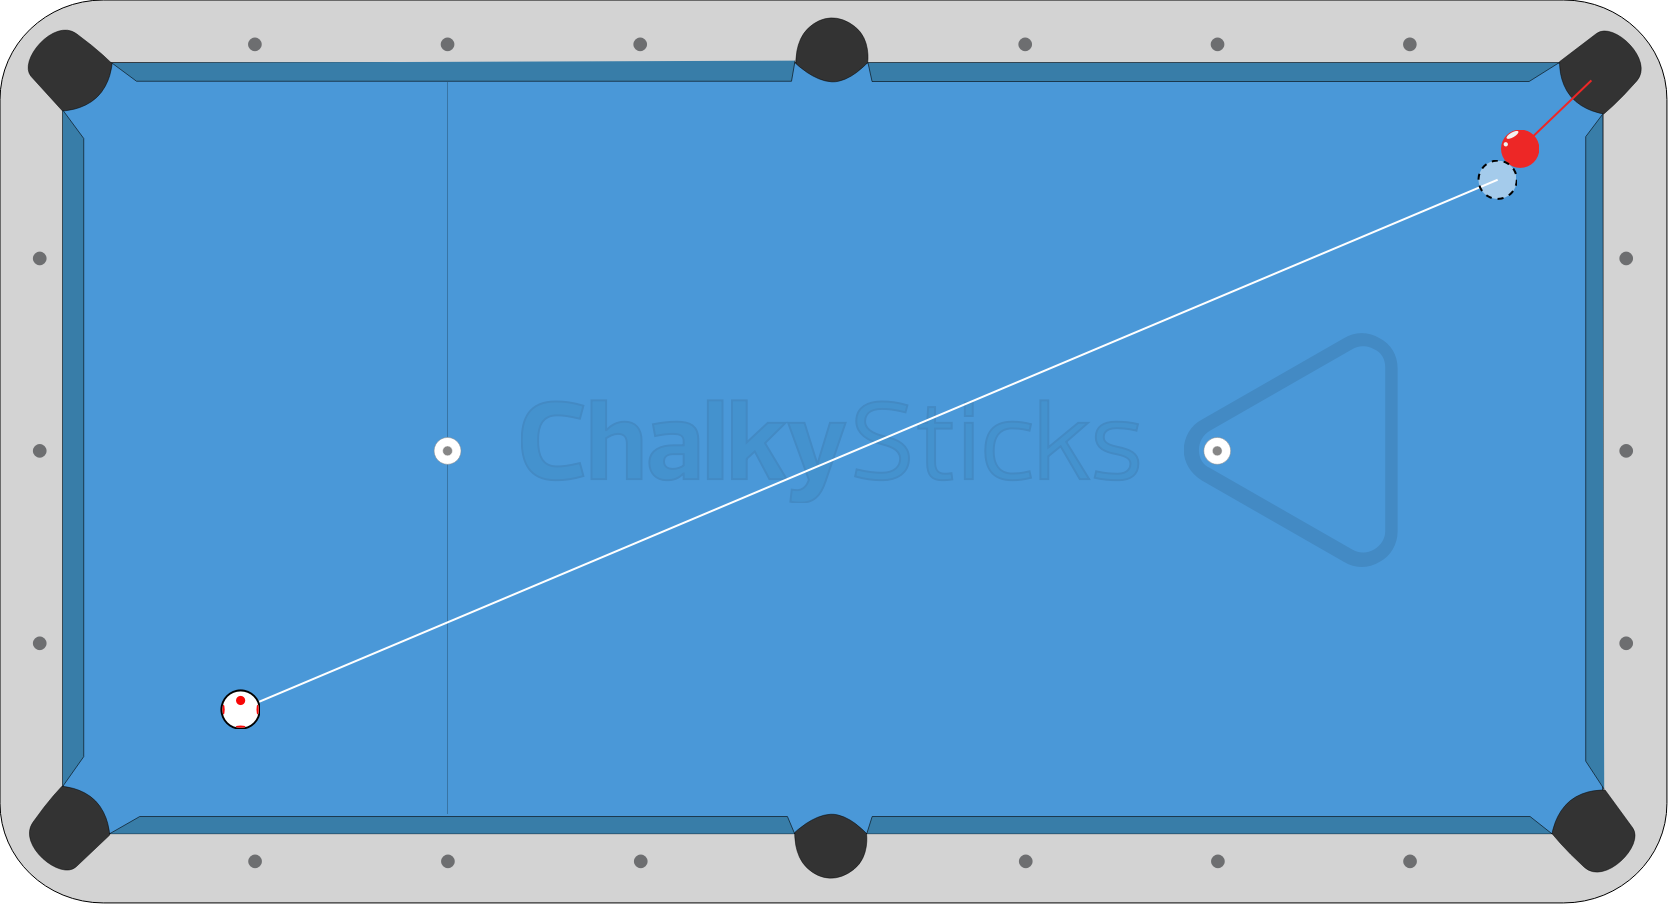
\includegraphics[scale = 0.2]{Images/Shot Diagrams/Shot_1.png}
    \caption{Shot 1 - An across table long shot.}
    \label{fig:shot1}
\end{figure}

\begin{figure}[h]
    \centering
    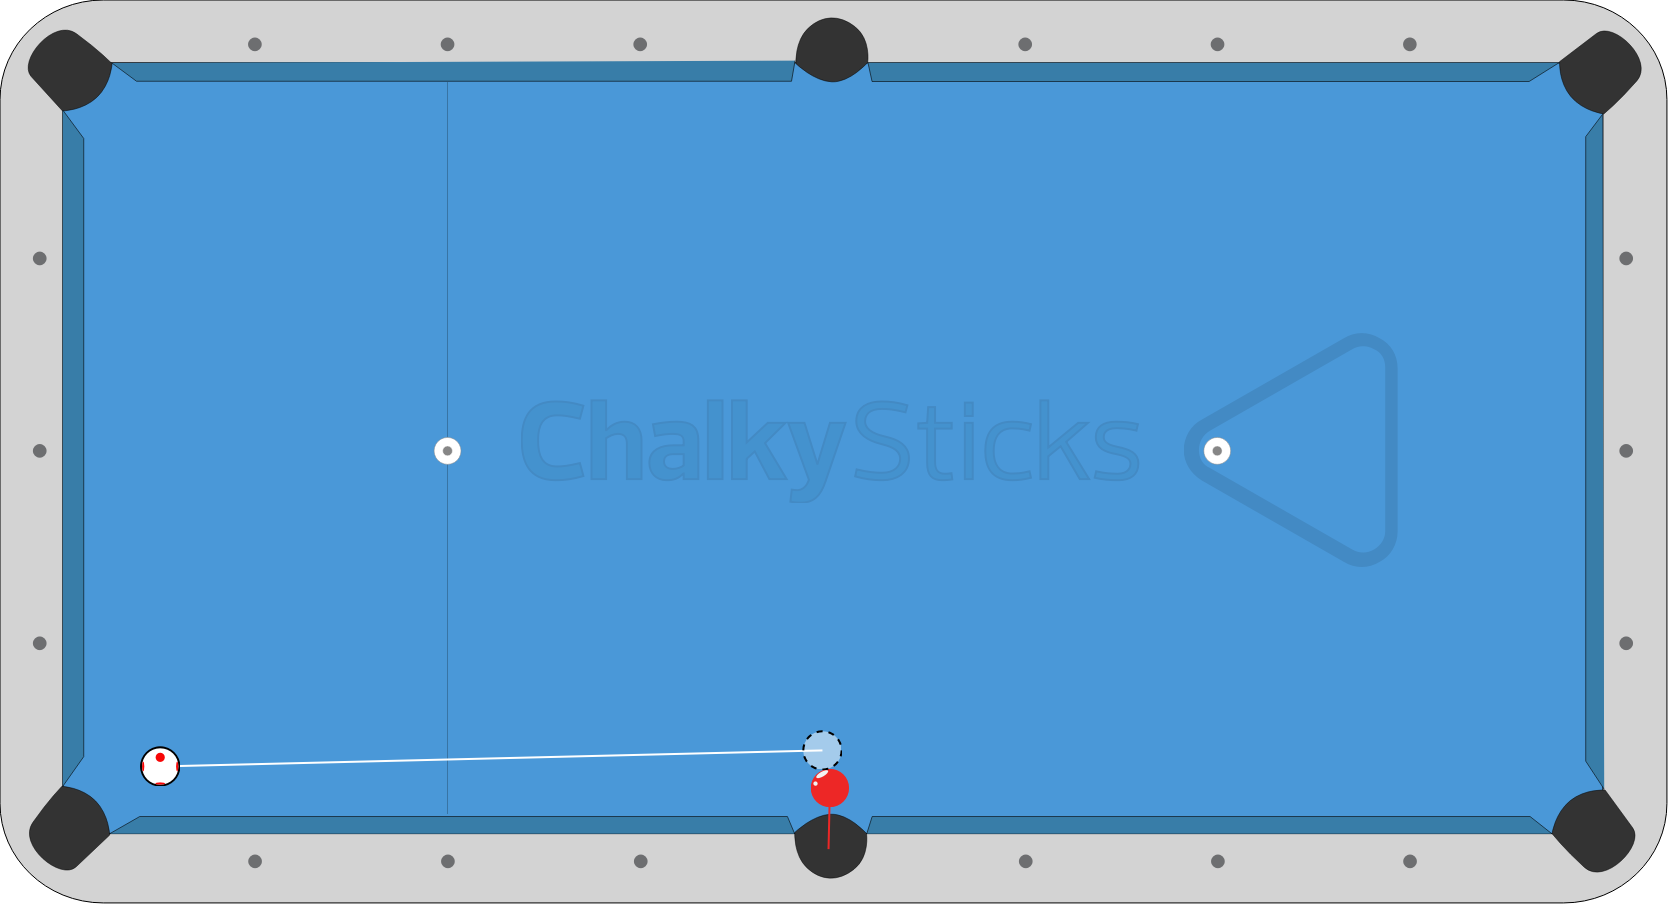
\includegraphics[scale = 0.2]{Images/Shot Diagrams/Shot_2.png}
    \caption{Shot 2 - A tight clip shot.}
    \label{fig:shot2}
\end{figure}

\begin{figure}[h]
    \centering
    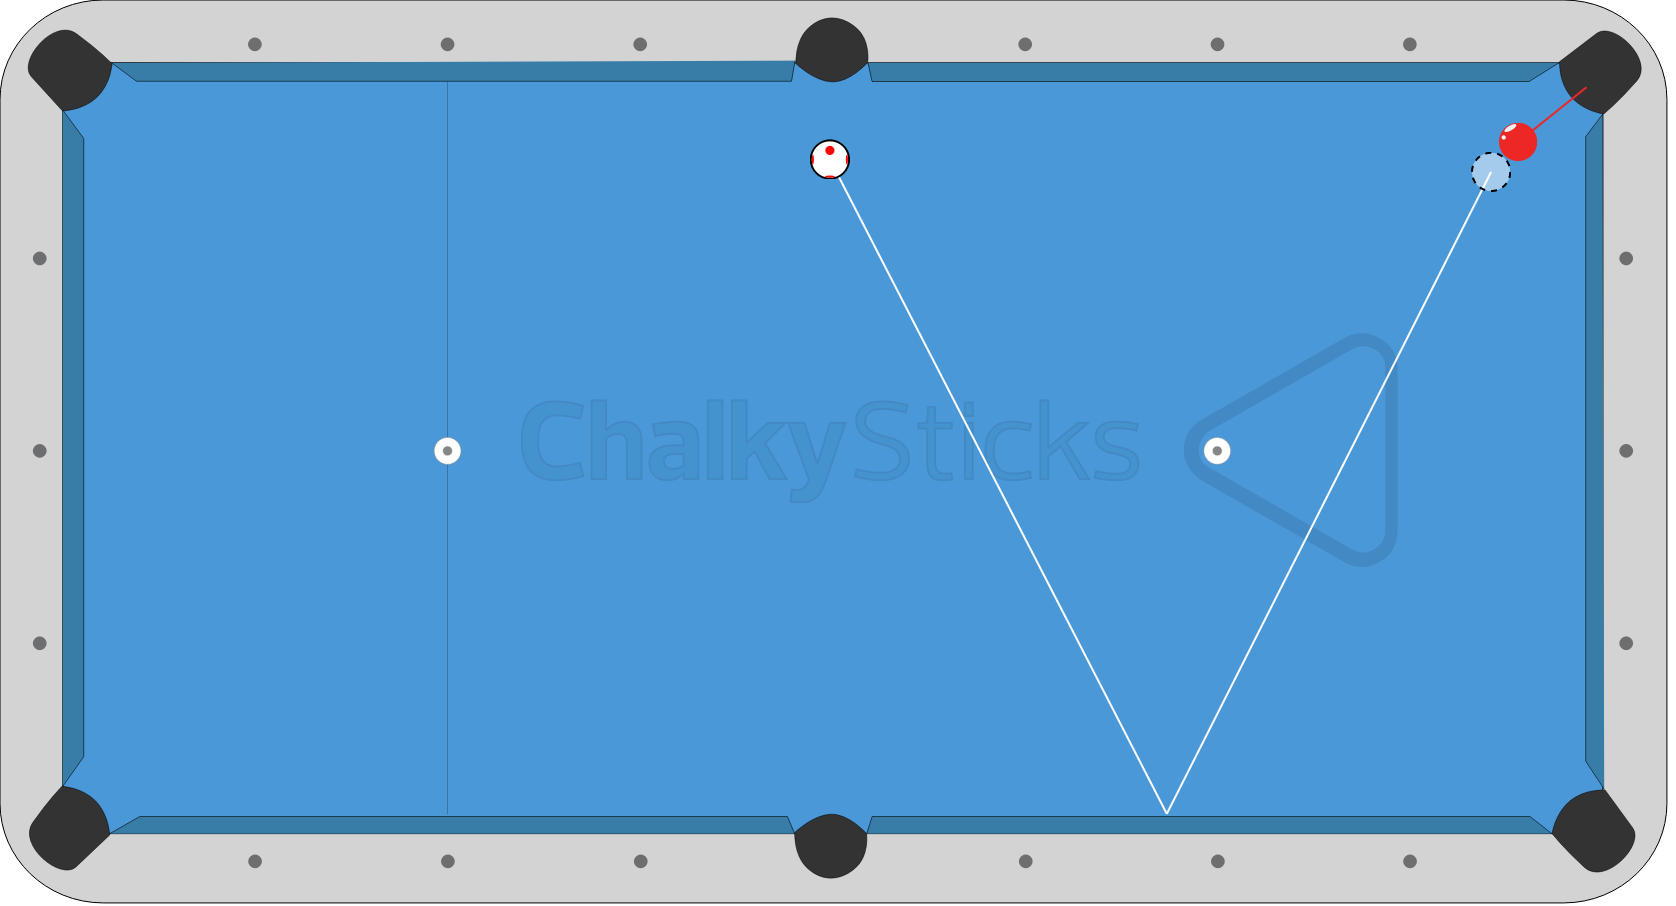
\includegraphics[scale = 0.2]{Images/Shot Diagrams/Shot_3.png}
    \caption{Shot 3 - A single rebound shot.}
    \label{fig:shot3}
\end{figure}

\begin{figure}[h]
    \centering
    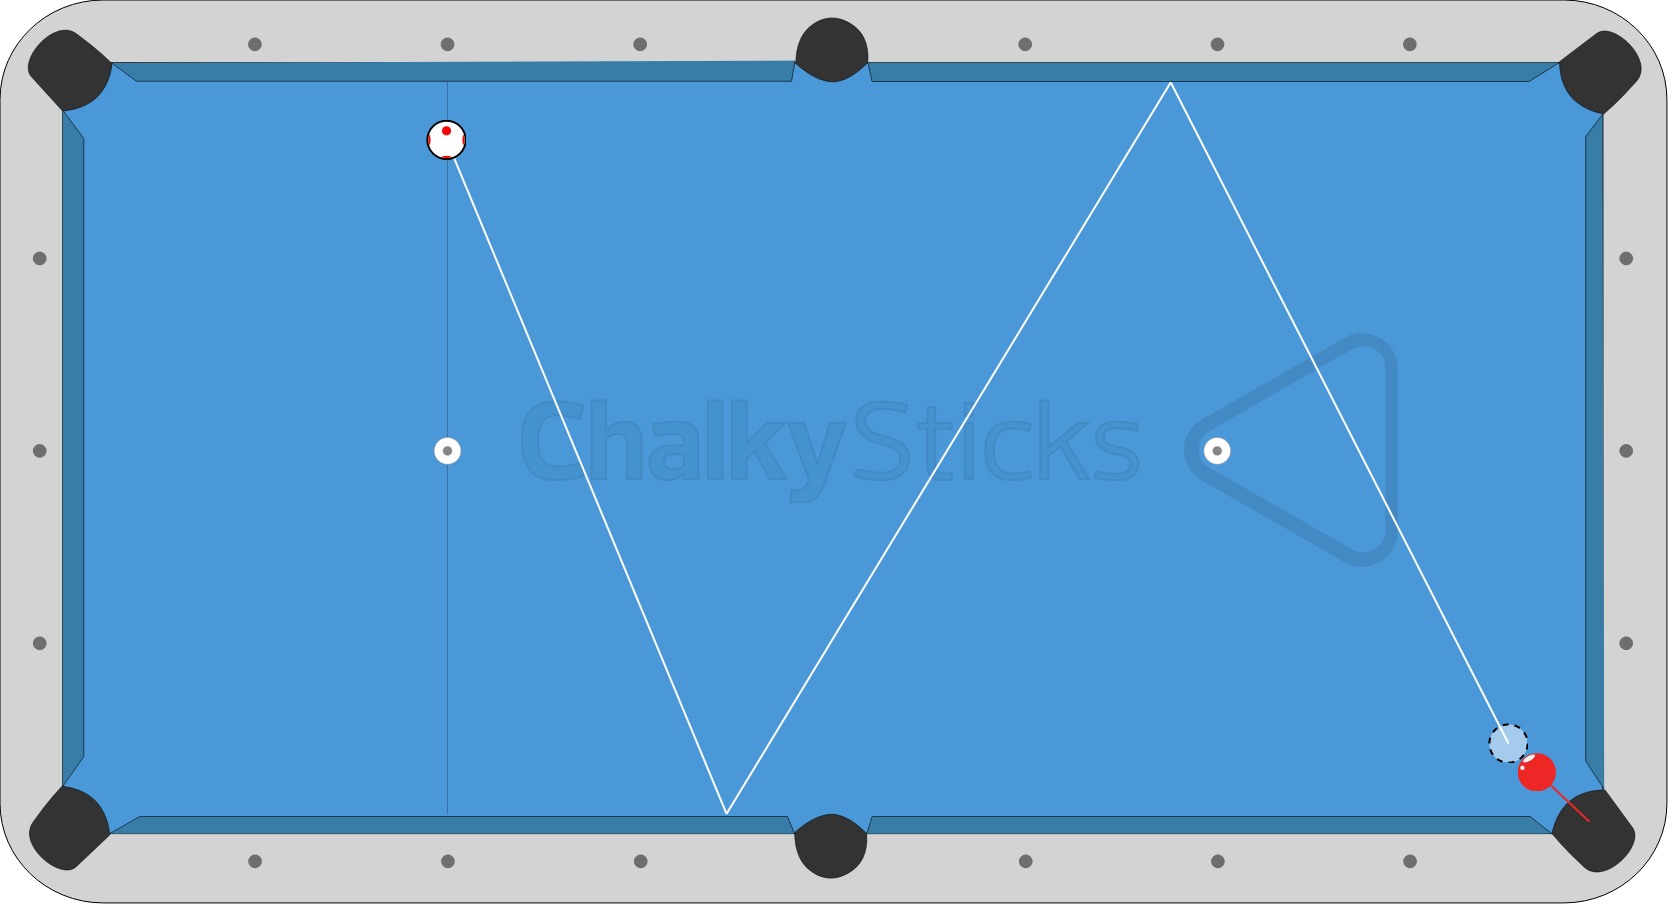
\includegraphics[scale = 0.2]{Images/Shot Diagrams/Shot_4.png}
    \caption{Shot 4 - A double rebound shot.}
    \label{fig:shot4}
\end{figure}

\begin{figure}[h]
    \centering
    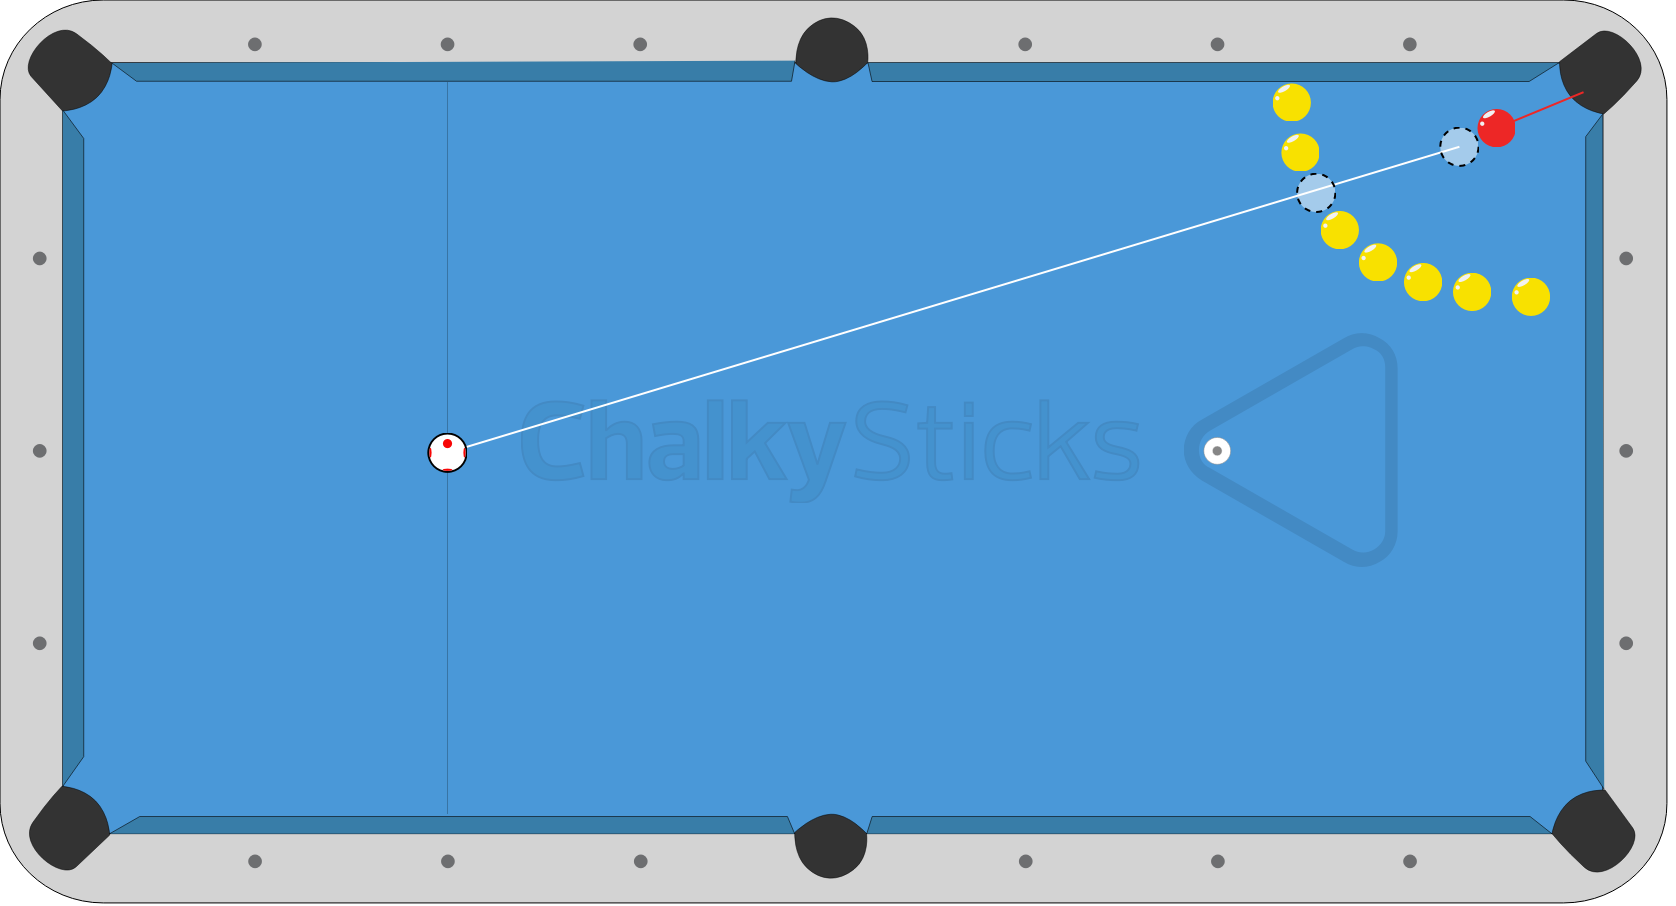
\includegraphics[scale = 0.2]{Images/Shot Diagrams/Shot_5.png}
    \caption{Shot 5 - A long shot requiring precise accuracy.}
    \label{fig:shot5}
\end{figure}

\begin{figure}[h]
    \centering
    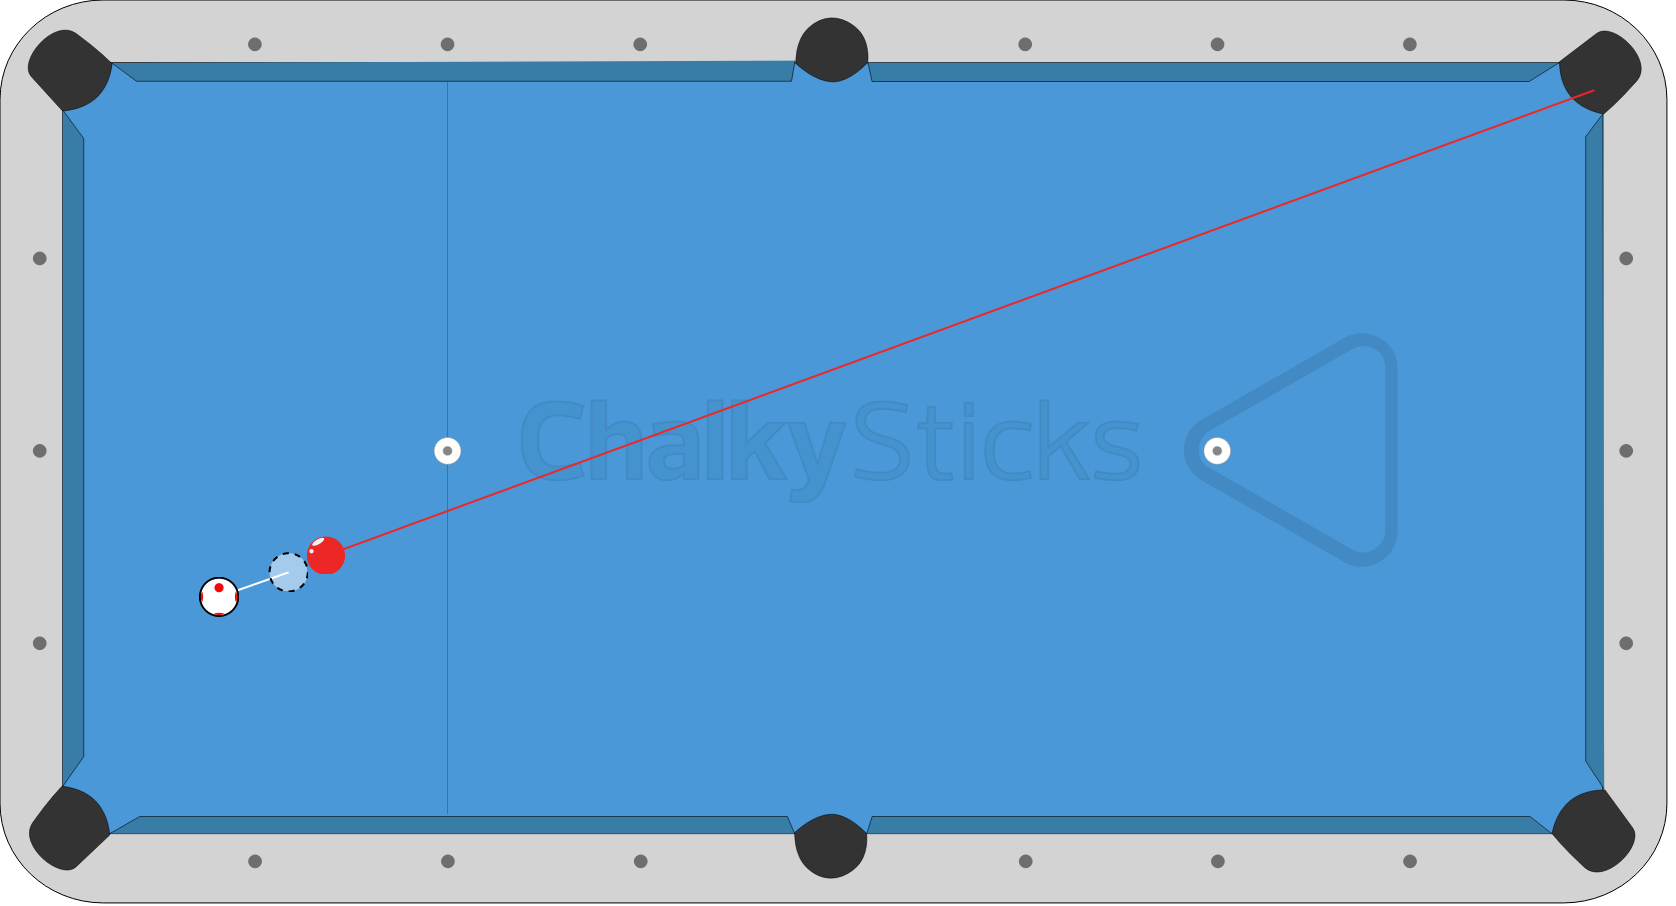
\includegraphics[scale = 0.2]{Images/Shot Diagrams/Shot_6.png}
    \caption{Shot 6 - A long shot with the target ball placed close to the cue ball.}
    \label{fig:shot6}
\end{figure}

\begin{figure}[h]
    \centering
    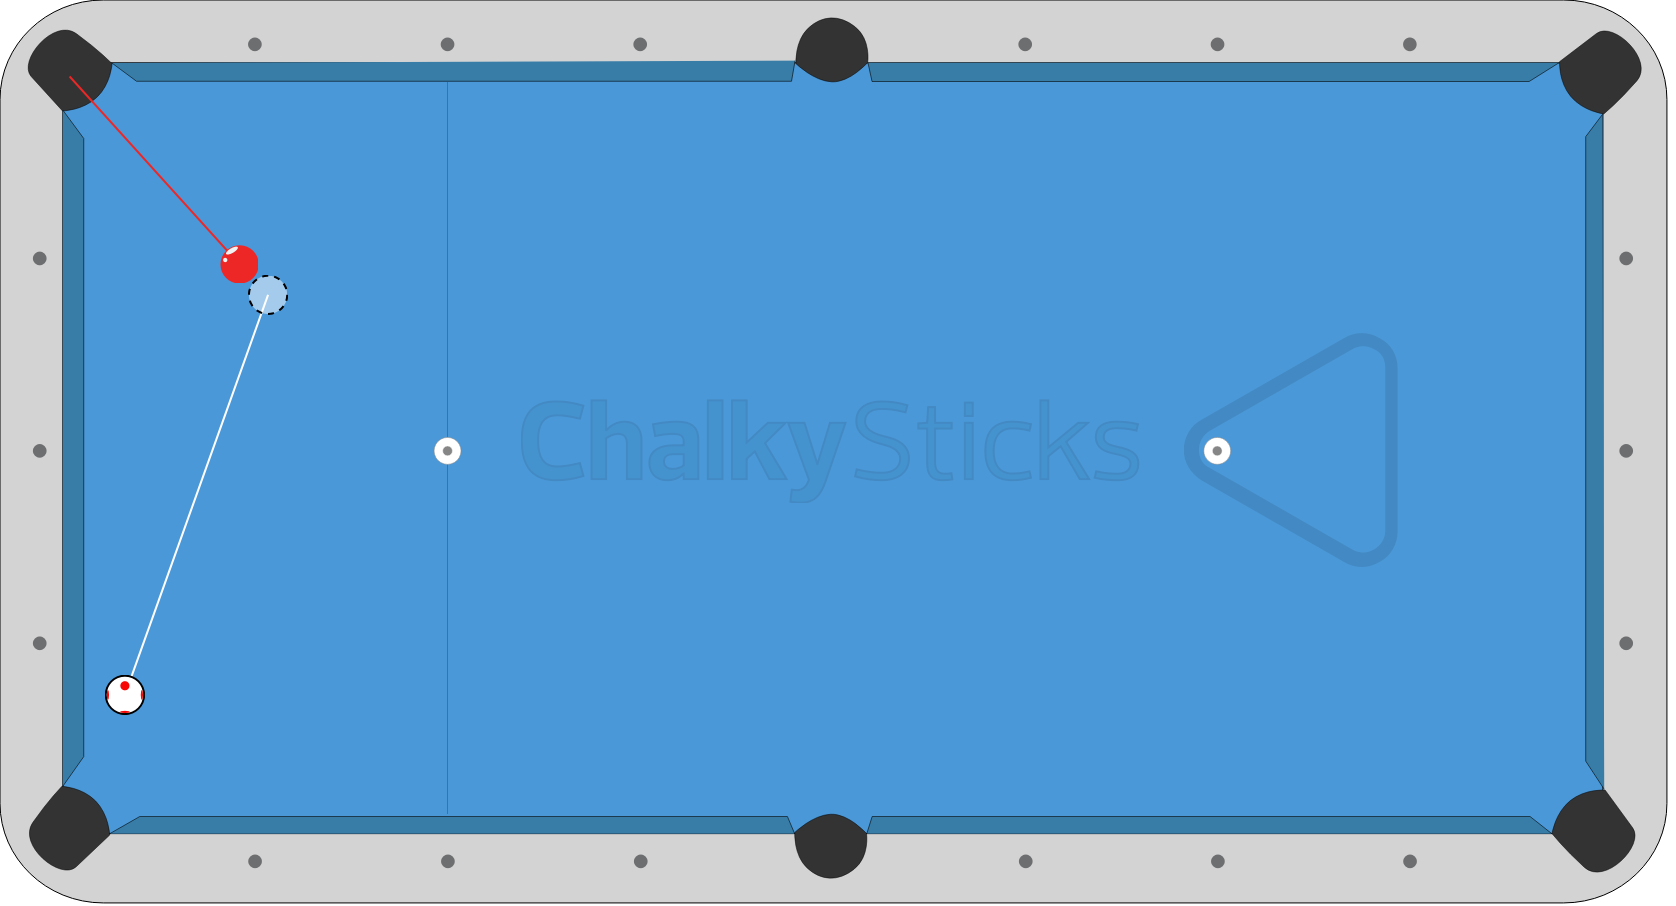
\includegraphics[scale = 0.2]{Images/Shot Diagrams/Shot_7.png}
    \caption{Shot 7 - A difficult cut back shot.}
    \label{fig:shot7}
\end{figure}


%-----------------------------------------------------------------------------------------------


\chapter{Post User Testing Questions}
\label{appx:userTestQuestions}
Detailed below are the questions I asked to each test user after they had completed all seven shots with and without my aim assistant application.
\begin{enumerate}
    \item From a scale of 1 to 10, how helpful did you find the Help Information inside the application? With 1 being not helpful at all, 10 being very helpful. 
    \item From a scale of 1 to 10, how intuitive was the application to use and navigate? With 1 being not intuitive at all, 10 being very intuitive.
    \item From a scale of 1 to 10, how easy was it to place the table model into place? With 1 being not easy at all, 10 being very easy.
    \item From a scale of 1 to 10, how easy was it to place the ball models into place? With 1 being not easy at all, 10 being very easy.
    \item From a scale of 1 to 10, how easy did you find it to move the hit marker and line up a shot? With 1 being not easy at all, 10 being very easy.
    \item Did you feel as though the application helped you to perform the activity better and was useful?
    \item What did you dislike the most about the application?
    \item What did you like the most about the application?
    \item Any additional comments or feedback?
\end{enumerate}


%-----------------------------------------------------------------------------------------------


\chapter{Post User Testing Transcripts}
\label{appx:userTestTranscripts}
Below are the transcripts between myself and each of the test users after they had used the system and completed various different shots.
\section{User 1}
\begin{tabular}{l p{130mm}}
    Myself : & Thanks for that. Can I ask you a few questions? \\
    User 1 : & Yeah sure.\\
    Myself : & Great, thanks. OK, from a scale of 1 to 10, how helpful did you find the Help Information inside the application? With 1 being not helpful at all, 10 being very helpful. \\
    User 1 : & Uhh a five.\\
    Myself : & Thank you. Next, from a scale of 1 to 10, how intuitive was the application to use and navigate? With 1 being not intuitive at all, 10 being very intuitive.\\
    User 1 : & Six.\\
    Myself : & OK. From a scale of 1 to 10, how easy was it to place the table model into place? With 1 being not easy at all, 10 being very easy.\\
    User 1 : & A four, it was hard to line it up exactly.\\
    Myself : & Thank you. From a scale of 1 to 10, how easy was it to place the ball models into place? With 1 being not easy at all, 10 being very easy.\\ 
    User 1 : & Seven. \\
    Myself : & Thank you. From a scale of 1 to 10, how easy did you find it to move the hit marker and line up a shot? With 1 being not easy at all, 10 being very easy. \\
    User 1 : & Seven again.\\
    Myself : & Great. Next, did you feel as though the application helped you to perform the activity better and was useful? \\
    User 1 : & Yes, for more difficult shots I had a better idea of where I had to aim. For the easier shots I didn't really notice a difference.\\
    Myself : & OK. Now, what did you dislike the most about the application? \\
    User 1 : & Positioning the table is quite difficult as the table doesn't fit on the screen all at the same time, so you have to keep walking round adjusting each corner which messes up other bits.\\
    Myself : & OK, and what did you like the most about the application? \\
    User 1 : & The aim assist thing was good.\\
    Myself : & Nice. And finally, do you have any additional comments or feedback? \\
    User 1 : & I think the headset is uncomfortable and a bit off-putting but the system it self is intuitive and very helpful.Because you cant see everything at once you have to keep looking away from the ball to see where the target is. When you compare it to VR everything you see is hologram but having half hologram half normal world is a bit weird.\\
    Myself : & Brill, that's it. Thanks again for helping me out and testing my app. \\
    User 1 : & No problem. \\
\end{tabular}

\section{User 2}
\begin{tabular}{l p{130mm}}
    Myself : & OK, we are done testing wise. Can I ask you a few questions? \\
    User 2 : & Yeah go ahead.\\
    Myself : & Great. First off, from a scale of 1 to 10, how helpful did you find the Help Information inside the application? With 1 being not helpful at all, 10 being very helpful. \\
    User 2 : & A six.\\
    Myself : & Thank you. Next, from a scale of 1 to 10, how intuitive was the application to use and navigate? With 1 being not intuitive at all, 10 being very intuitive.\\
    User 2 : & Again a six.\\
    Myself : & From a scale of 1 to 10, how easy was it to place the table model into place? With 1 being not easy at all, 10 being very easy.\\
    User 2 : & Four.\\
    Myself : & From a scale of 1 to 10, how easy was it to place the ball models into place? With 1 being not easy at all, 10 being very easy.\\ 
    User 2 : & Eight.\\
    Myself : & OK, from a scale of 1 to 10, how easy did you find it to move the hit marker and line up a shot? With 1 being not easy at all, 10 being very easy. \\
    User 2 : & A five.\\
    Myself : & Next, did you feel as though the application helped you to perform the activity better and was useful? \\
    User 2 : & I thought knowing where the white ball will go was useful to know, but, I mean, I don’t think it made me any better as I got more in without it aha.\\
    Myself : & Aha right, thanks. What did you dislike the most about the application? \\
    User 2 : & Moving the balls and cue marker was very sensitive and made it hard sometimes to place things accurately.\\
    Myself : & What did you like the most about the application? \\
    User 2 : & The white line showing where the balls will go, I thought it was really good!\\
    Myself : & OK and finally, do you have any additional comments or feedback? \\
    User 2 : & The headset feels like its in the way sometimes and it would be nicer if there was a bigger screen so you could see everything at the same time. I thought the app was good but a few things could be done to improve it.\\
    Myself : & What exactly do you think could be done to improve it? \\
    User 2 : & Maybe something to place the table and balls automatically? I think that would be the biggest thing.\\
    Myself : & Great that's it!. Thanks again for helping me out. \\
    User 2 : & My pleasure. \\
\end{tabular}

\section{User 3}
\begin{tabular}{l p{130mm}}
    Myself : & Thank you for testing out my application. Would I be able to ask you a few questions? \\
    User 3 : & Yes of course.\\
    Myself : & Great. Firstly, from a scale of 1 to 10, how helpful did you find the Help Information inside the application? With 1 being not helpful at all, 10 being very helpful. \\
    User 3 : & I'd say an eight. It helped me figure out what to do but could have been presented in a better way.\\
    Myself : & OK cool. Next, from a scale of 1 to 10, how intuitive was the application to use and navigate? With 1 being not intuitive at all, 10 being very intuitive.\\
    User 3 : & Again I'd say an eight.\\
    Myself : & OK thanks. From a scale of 1 to 10, how easy was it to place the table model into place? With 1 being not easy at all, 10 being very easy.\\
    User 3 : & A seven. It wasn't that hard but took a little while to line it up properly.\\
    Myself : & Thank you. From a scale of 1 to 10, how easy was it to place the ball models into place? With 1 being not easy at all, 10 being very easy.\\ 
    User 3 : & A nine, it was very easy to place them into position. \\
    Myself : & Thank you. From a scale of 1 to 10, how easy did you find it to move the hit marker and line up a shot? With 1 being not easy at all, 10 being very easy. \\
    User 3 : & Nine for sure. I found the plus 1 degree and minus 1 degree buttons really useful to finalise it's position after I got it nearly into place. \\
    Myself : & That's great! Next, did you feel as though the application helped you to perform the activity better and was useful? \\
    User 3 : & Yes it was very helpful, especially on shot 5. \\
    Myself : & OK, now, what did you dislike the most about the application? \\
    User 3 : & Moving the hit marker into position as it was very sensitive to any movement, even very small ones, and it was quite hard to grab onto sometimes. \\
    Myself : & OK thank you. What did you like the most about the application? \\
    User 3 : & The trajectory shown is quite accurate actually. It defiantly helped me to pot the balls better! The headset itself and making gestures like you're actually grabbing something is really cool too! \\
    Myself : & It's great isn't it! And finally, do you have any additional comments or feedback? \\
    User 3 : & I think making the hit marker less sensitive to movement and when you were taking a shot would be good. You also cant really see the rest of the table or where the ball will go when you're trying to take a shot as the screen is not aligned with your line of sight. But it make me want to play pool more in real life! I really enjoyed it! \\
    Myself : & That's great. Thank you again for testing out the application! \\
    User 3 : & You're welcome. It was great fun! \\
\end{tabular}

\section{User 4}
\begin{tabular}{l p{130mm}}
    Myself : & OK, we're all done. Can I ask you a few questions? \\
    User 4 : & Of course!\\
    Myself : & Great. From a scale of 1 to 10, how helpful did you find the Help Information inside the application? With 1 being not helpful at all, 10 being very helpful. \\
    User 4 : & A three, it was kinda hard to read.\\
    Myself : & Thank you. From a scale of 1 to 10, how intuitive was the application to use and navigate? With 1 being not intuitive at all, 10 being very intuitive.\\
    User 4 : & Seven.\\
    Myself : & From a scale of 1 to 10, how easy was it to place the table model into place? With 1 being not easy at all, 10 being very easy.\\
    User 4 : & A one, I found it very hard!\\
    Myself : & Thank you. From a scale of 1 to 10, how easy was it to place the ball models into place? With 1 being not easy at all, 10 being very easy.\\ 
    User 4 : & A five, much easier than the table!\\
    Myself : & From a scale of 1 to 10, how easy did you find it to move the hit marker and line up a shot? With 1 being not easy at all, 10 being very easy. \\
    User 4 : & A six, it was a bit sensitive but the buttons helped a lot.\\
    Myself : & Next, did you feel as though the application helped you to perform the activity better and was useful? \\
    User 4 : & Yes it was helpful as long I was able to line up the shot properly.\\
    Myself : & What did you dislike the most about the application? \\
    User 4 : & Having to move the objects, but most of all line up the shot by dragging the cue marker. The help text was also kinda hard to read.\\
    Myself : & And what did you like the most about the application? \\
    User 4 : & That it explains it very well and that I hit more balls with it on!\\
    Myself : & OK and finally, do you have any additional comments or feedback? \\
    User 4 : & I think that it is very smart application and if it was easier to use it would be more welcomed, but I wouldn't use it myself as I found it too hard to move things into place and line up the shots. I was wondering whether I was placing the ball correctly or not as there is a lot of human error so I put a lot of focus on moving the ball maybe more than I should have just so it lines up correctly. The lines did help to visualise the shot a lot. When I usually play I do imaginary lines to line up my shots but with the HoloLens it displays them for me which I found useful. It would be useful if it put everything in place for me! I also Started to get a headache. \\
    Myself : & Great. Thank you very much for your help and feedback. \\
    User 4 : & No worries! It was fun to use but a little frustrating aha. \\
\end{tabular}

% =============================================================================

\end{document}
